\documentclass[twoside,bibliography=totoc,openany,numbers=noenddot]{fumi}

% Definition von Variablen
\newcommand{\thesistitle}{Repräsentation von Kurseinheiten der FernUniversität als Hyperaudio-Dokumente in Moodle: Design und Implementierung}
\newcommand{\thesisauthor}{Michael Lämmermann}
\newcommand{\thesistype}{Bachelorarbeit} % Bachelorarbeit, Diplom, Masterarbeit, ects.
\newcommand{\thesismatrikelnummer}{9611711}

% Tell LaTeX about how to wrap words using the correct german hyphenation rules.
\hyphenation{Lern-arrange-ments Lern-arrange-ment Lern-aktivität Lern-aktivitäten doku-mentiert Hash-funk-tion Hash-funk-tionen Video-frames Video-frame Link-ak-ti-vier-ung Co-decs Link-ob-jekt-es  Hyper-video-Autoren-um-geb-ung-en  App-li-kat-ion-en  Kon-tain-er-for-mat Bild da-tei-en  Co-decs Brow-ser   Au-to-ren-um-ge-bun-gen Aus-zeich-nungs-spra-che spe-zi-fische Vi-deo-lern-um-ge-bung-en Vi-deo-lern-um-ge-bung Lern-um-ge-bung Lern-um-ge-bung-en Hy-per-au-dio-Do-ku-ment Hy-per-au-dio-Do-ku-men-te Hy-per-au-dio Do-ku-ment Do-ku-men-te wave-sur-fer Fern-Uni-ver-si-tät Auf-lis-tung Tab-let Zu-satz-in-hal-te}

\title{\thesistitle}
\author{\thesisauthor}
\date{\today}

%%%%%%%%%%
\captionsetup[figure]{justification=centering}
%\captionsetup[table]{justification=left}
\captionsetup[subfigure]{labelformat=brace}
\newcommand\Subref[3][]{%
   \ref{#2}(\subref{#3}%
   \ifthenelse{\equal{#1}{}}{}{-\subref{#1}}%
   )}
%%%%%%%%%%
\usepackage{courier}
\usepackage{xcolor}
\usepackage{textcomp}
\colorlet{punct}{red!60!black}
\definecolor{delim}{RGB}{20,105,176}
\definecolor{commentgreen}{RGB}{2,112,10}
\definecolor{eminence}{RGB}{108,48,130}
\lstdefinelanguage{json}{
    literate=
     *{:}{{{\color{punct}{:}}}}{1}
      {,}{{{\color{punct}{,}}}}{1}
      {\{}{{{\color{delim}{\{}}}}{1}
      {\}}{{{\color{delim}{\}}}}}{1}
      {[}{{{\color{delim}{[}}}}{1}
      {]}{{{\color{delim}{]}}}}{1},
}
\lstdefinelanguage{css}{
    keywordstyle=\color{eminence}, % 
    morekeywords={@media, div, input}
}
\lstset {
    language=php,
    aboveskip=15pt,
    columns=fullflexible,
    basicstyle=\ttfamily\footnotesize,
    numbers=left,
    numberstyle=\scriptsize,
    stepnumber=1,
    numbersep=8pt,
    showstringspaces=false
    breaklines=true,
    frame=lines,
    extendedchars=false,
    upquote=true,
    %escapeinside=\``,
    inputencoding={utf8}, 
    commentstyle=\color{commentgreen},
    keywordstyle=\color{eminence},
    stringstyle=\color{blue},
    emph={int,char,double,float,unsigned,void,bool},
    emphstyle={\color{blue}},
    classoffset=1, % starting new class
    otherkeywords={.,;,-,!,~,null,function},
    morekeywords={.,;,-,!,~,null,function},
    deletekeywords={header},
    classoffset=0,
}
\usepackage{letltxmacro}
% https://tex.stackexchange.com/q/88001/5764
\LetLtxMacro\oldttfamily\ttfamily
\DeclareRobustCommand{\ttfamily}{\oldttfamily\csname ttsize\endcsname}
\newcommand{\setttsize}[1]{\def\ttsize{#1}}%
%%%%%%%%%%
\usepackage{rotating}
\usepackage{enumitem}
\usepackage{longtable}
\usepackage{underscore}
\usepackage{placeins}
%\usepackage{microtype}
%%%%%%%%%%

%%%%%%%%%%%%%%%%%%%%%%
\begin{document}
\sffamily
\pagestyle{empty}
\setttsize{\small}


%% Titelseite (optional für die PDF-Version des Textes)
%\includepdf[pages=-, offset=0 0]{img/cover.pdf}\newpage~\newpage

%% Die erste Seite eines Buches
%\thesisauthor\\{\textbf{\thesistitle}}\vfill\newpage~\newpage

%% Die Seite mit den Titelangaben
\vspace{2cm}
\begin{center}\LARGE
\vfill
{\Huge\thesistitle}\\
\vfill
\thesistype\\
\vfill
eingereicht von\\[4pt]
\textbf{\thesisauthor}\\[4pt]
(Matrikelnummer \thesismatrikelnummer)\\
\vfill
angefertigt am\\
Lehrgebiet Kooperative Systeme\\
Fakultät Mathematik und Informatik\\
FernUniversität in Hagen\\
\vfill 
Betreuer\\
Dr. Niels Seidel
\vfill
\monthname[\the\month] \the\year
\end{center}
\newpage~\newpage

%% Leerseite mit Titel
{\large\textbf{\thesisauthor}\\\textbf{\thesistitle}\vfill}\newpage~\newpage


%% Seite mit Zusammenfassung und englishsprachigen Summary
\section*{Zusammenfassung}
Aktuell werden Lerninhalte an der FernUniversität in Hagen hauptsächlich in Form von textlastigen Kurseinheiten vermittelt. Diese schränken die Studierenden, bezogen auf die Tätigkeiten, welche beim Lernen durchgeführt werden können, ein. Aus diesem Grund lässt sich das Lernen aktuell schwer in Alltagstätigkeiten integrieren. Ziel dieser Arbeit soll es sein, eine auditive Lernumgebung zu schaffen, welche alle Inhalte der bestehende Kurseinheiten vermitteln kann. Die auditive Lernumgebung soll es den Studierenden ermöglichen, zukünftig mehr Zeit zum Lernen wahrzunehmen. Um dieses Ziel zu erreichen, wird ein Moodle-Plugin entwickelt, welches eine alternative Repräsentation der Kurseinheiten bietet und zudem Kommunikationsmöglichkeiten für Studierende und Lehrende schafft.\vfill
\section*{Summary}
Currently, learning content is primarily provided in the form of text-heavy course units at the FernUniversität in Hagen. Those restrict the students in terms of activities which can be executed during studying. For that reason learning is currently difficult to integrate in everyday activities. The goal of this work is to create an auditory learning environment imparting all the content of the existing course units. The auditory learning environment should enable students to use more time for studying. In order to reach this goal, a Moodle plugin is developed, offering an alternative representation for course units while also creating the means for communication between students and teachers.
\vfill\newpage

%% Seite mit bibliografischen Angaben
{\small
%Herausgeber: Namen der Herausgeber\\

% Zitation
\thesisauthor. \textit{\thesistitle}. \thesistype. Fakultät Mathematik und Informatik, FernUniversität in Hagen, \the\year. %\href{}{}. % optional URN
\\\vfill

% Optional, jedoch sehr zu empfehlen
Diese Publikation ist unter \emph{Creative Commons -- Namensnennung 3.0 Deutschland} lizenziert und darf als Ganzes oder ausschnittweise vervielfältigt, verbreitet und öffentlich zugänglich gemacht werden, sofern dies im Text nicht anders vermerkt ist.\newline\vspace{10pt}
\hspace{-9pt}
\includegraphics[height=10mm]{logo-cc.pdf}
\\\vspace{10pt}

% ISBN: \dots\\
% URN: \href{...}
Autor: \thesisauthor\\
Gestaltung und Satz: \thesisauthor / \LaTeX\\
% Lektorat: Claudia Neumann\\ optional
% Titelbild: \dots\\optional
Datum: \today\\
% Printed in Germany
\cleardoublepage
}

%% Inhaltsverzeichnis
\pagestyle{headings}
\tableofcontents

\clubpenalty10000
\widowpenalty10000
\displaywidowpenalty=10000

%%%%%%%%%%%%%%%%%%%%%%%%%%%%%%%%%%%%%%%%%%%%%%%%%%%
\begin{sloppypar}
\chapter{Einführung}
%% lade Kapitel aus Datei

\label{cha:einfuehrung}
Diese Arbeit beschäftigt sich mit dem Design und der Implementierung eines Plugins für die Lernplattform Moodle, welches es ermöglichen soll, den Studierenden die Lerninhalte mittels Hyperaudio"=Dokumenten bereitzustellen. Ziel dieses Plugins ist die Erweiterung der Lernmöglichkeiten an der FernUniversität in Hagen, um die Studierenden beim Erreichen ihrer Lernziele besser zu unterstützen. 


%%%%%%%%%%
\section{Motivation}
\label{sec:motivation}
Die Motivation zur Behandlung dieses Themas besteht darin, dass 
%ca. 80\% der Studierenden in Teilzeit studieren und 
80\% der Studierenden neben dem Studium ebenfalls einer Arbeit nachgehen \citep{fernuniversitaet2018stat}. Unter diesen Umständen beschäftigen sich viele Studierende erst kurz vor der Prüfung - dafür aber entsprechend intensiv - mit den Lerninhalten. An der Fakultät Mathematik/Informatik und auch an der Fakultät für Wirtschaftswissenschaften bestehen diese Lerninhalte zu einem guten Teil aus textlastigen Kurseinheiten, die Abbildungen und Formeln enthalten.\\
Diese Aussage kann anhand der Pflichtmodule des Bachelorstudiengangs Wirtschaftsinformatik bestätigt werden. Die Pflichtmodule an der Faktultät Mathematik/Informatik weisen einen Textanteil von 61,08\% auf. An der Fakultät für Wirtschaftswissenschaften liegt der Anteil in den Pflichtmodulen nochmals höher bei 64,24\%\footnote{Genauere Informationen zu dieser Auswertung können im Anhang \ref{sec:TextanteilDerKurseinheiten} nachgeschlagen werden.}.

Eher selten werden auch Videos angeboten, in welchen bestimmte Lerninhalte aus den Kurseinheiten nochmals rekapituliert werden. Hier sind als Beispiel die Videos von Univ.-Prof. Dr. Ulrike Baumöl zum Kurs \glqq Informationsmanagement\grqq{} zu nennen.

Die Idee besteht nun darin, den Lernenden erstens eine alternative Repräsentation (Modalität) der Lerninhalte anzubieten und ihnen zweitens das Lernen während ungenutzter Alltagssituationen zu ermöglichen (z.B. lange Autofahrten, Pendeln in Bus und Bahn, beim Joggen, etc.). Auf diese Weise könnten die Lernenden die Inhalte häufiger rezipieren und einüben. Ergänzt um gute E-Assessments (Selbsttests) hätten sie in Summe eine Chance, sich frühzeitig und kontinuierlich auf die Prüfung vorzubereiten und vielleicht bessere Lernerfolge zu erzielen. 


%%%%%%%%%
\section{Problemstellung}
Diese Arbeit wird sich in diesem Zusammenhang vor allem mit dem Problem des hohen Textanteils vieler Kurse und dem damit verbundenen Lernverhalten beschäftigen. Doch zunächst soll die Ist-Situation für die Studierenden an der FernUniversität in Hagen beschrieben werden.

%%%%%%%%%
\subsection{Ist-Situation}
Jeder Studierende hat Zugriff auf den \textit{Virtuellen Studienplatz}, häufig auch \textit{Virtuelle Universität} (VU) oder \textit{Lernraum Virtuelle Universität} (LVU) genannt. Hierbei handelt es sich um ein eigenentwickeltes Webportal der FernUniversität in Hagen. Der \textit{Virtuelle Studienplatz} stellt unter anderem das Kurs- und Studiumsportal der FernUniversität dar. Hierüber können die Studierenden Kurse belegen, die Rückmeldung für das nächste Semester vornehmen oder ihre persönlichen Daten einsehen und bearbeiten. Auch eine Übersicht über das Veranstaltungsangebot wird dem Studierenden geboten. Zusätzlich bietet der \textit{Virtuelle Studienplatz} eine Übersicht über alle belegten Kurse des Studierenden \citep{fernuniversitaet2018vu}. Mittels dieser Übersicht kann der Studierende direkt auf das jeweilige persönliche Kursportal seiner belegten Kurse gelangen. Neben allgemeinen Informationen zu dem Kurs bietet das Kursportal unter anderem Zugriff auf die Online-Studieninhalte (z.B. Kurseinheiten\footnote{Kurseinheiten werden an der FernUniversität in Hagen auch als Studienbriefe bezeichnet.}, Einsendeaufgaben, Musterlösungen) und Verweise zu anderen Diensten (Moodle, Online-Übungssystem, Kommunikationsangebote Adobe Connect Videokonferenzen), die in diesem Kurs zur Verfügung stehen \citep{fernuniversitaet2018kurs}.

Neben der Möglichkeit, die Kurseinheiten als PDF (Portable Document Format) über den \textit{Virtuellen Studienplatz} herunterzuladen, werden diese im Regelfall für die belegten Kurse automatisch in gedruckter Form an die Studierenden versendet. Die Kurseinheiten dienen als zentrales Lernmaterial für die Studierenden.

Jeder Kurs hat die Möglichkeit, zusätzliches Lernmaterial über Moodle, die zentrale Lernplattform der FernUniversität in Hagen, zur Verfügung zu stellen. Moodle bietet den Kursen \glqq als sogenanntes Learningmanagementsystem (LMS) vielfältige Möglichkeiten zur Gestaltung der mediengestützten Lehre an\grqq{} \citep{fernuniversitaet2018moodle}. Besonders hervorzuheben ist hierbei der mögliche Einsatz von Lehrvideos, Foren und Tests. Die Platttform Moodle und ihre Erweiterungsmöglichkeiten werden in Abschnitt \ref{sec:moodle} vorgestellt. Im Bezug auf die Pflichtmodule des Bachelorstudiengangs Wirtschaftsinformatik an der FernUniversität in Hagen wird Moodle in 21 von 30 Kursen beziehungsweise 10 von 15 Modulen eingesetzt (vgl. Anhang \ref{sec:EinsatzVonMoodle}). Auffällig ist dabei, dass während Moodle an der Fakultät für Wirtschaftswissenschaft für jeden Kurs angeboten wird, an der Fakultät für Mathematik und Informatik kein einziger Kurs der Pflichtmodule des Bachelorstudiengangs Wirtschaftsinformatik auf Moodle zurückgreift.

Durch den Einsatz von Adobe Connect besteht an der FernUniversität in Hagen auch die Möglichkeit sogenannter \textit{Virtual Classrooms}. Dabei handelt es sich um eine Video- und Tonübertragung mit Textchat und Freigabemöglichkeiten für Präsentationen und Bildschirminhalte. \glqq Ein \emph{Virtual Classroom} [Hervorhebung v. Verf.] eignet sich insbesondere für Veranstaltungen, in denen die synchrone Kommunikation ein hohes Gewicht erhält: Seminare, Tutorien, Sprechstunden, Arbeitsgruppen u.Ä.\grqq{} \citep{fernuniversitaet2018kommunikationstools}.

Darüber hinaus werden den Studierenden mit den \textit{Diskussionsforen} (Newsportal) und dem \textit{Conference Center} als Chat-System zwei weitere Systeme zur Kommunikation geboten \citep{fernuniversitaet2018kommunikationstools}.


%%%%%%%%%
\subsection{Probleme}
Die im vorangegangen Abschnitt beschriebenen Lernangebote weisen jedoch Defizite im Bezug auf die Vermittlung der Lerninhalte auf. Der \textit{Virtuelle Studienplatz} dient aktuell ausschließlich als Portal, um die Studierenden zu den von ihnen benötigen Informationen zu leiten und unterstützt somit nur indirekt die Vermittlung von Lerninhalten.

Die Kurseinheiten als zentrales Lernmaterial bestehen, wie anhand der Zahlen aus Abschnitt \ref{sec:motivation} erkenntlich, zum Großteil aus Text. Dies hat zur Folge, dass sich die Studierenden während der Auseinandersetzung mit den Lerninhalten nicht mit anderen Dingen beschäftigen können, welche die Aufmerksamkeit ihrer Augen und Hände benötigen. Zusätzlich besteht oft das Problem, dass Abbildungen, Formeln und Tabellen, auf die im Text verwiesen wird, nicht direkt auf der Seite ersichtlich sind, auf der diese im Text erwähnt werden. Hierdurch ist oftmals Blättern bzw. Scrollen nötig, je nachdem ob die Kurseinheit in Papierform oder digital bearbeitet wird. Dies erschwert zusätzlich das Verinnerlichen des in der Kurseinheit zu vermittelnden Inhalts \citep{mayer2009multimedia}. Im Vergleich zum Frontalunterricht bringt die Vermittlung der Lerninhalte in Form von Kurseinheiten den Nachteil mit sich, dass bei Verständnisproblemen keine direkten Fragen gestellt werden können.

Dieses Problem tritt bei Lehrvideos ebenso auf. Hier ist im besten Fall ein asynchroner Austausch mittels einer Kommentarfunktion möglich. Ähnlich wie Kurseinheiten verlangen auch Lehrvideos die durchgehende visuelle Aufmerksamkeit des Studierenden. Nur durch ununterbrochenes Betrachten eines Videos kann ein Studierender sicherstellen, dass er alle dargestellten Inhalte wahrnimmt.

Im Gegensatz zu Lehrvideos, sind die Foren und der Chat ohnehin nur als zusätzliche Kommunikationswege für die Studierenden implementiert. Es besteht das grundsätzliche Problem, dass diese Funktionalitäten nicht direkt an die Lerninhalte gekoppelt sind und deswegen separat aufgerufen werden müssen, falls beim Lernen Fragen auftreten sollten. 

Die in Moodle verfügbaren Tests dienen hingegen in ihrer Form nur zur reinen Selbstkontrolle. Dadurch, dass diese Tests nicht direkt während der Erarbeitung der Lerninhalte durch Kurseinheit oder Lehrvideos erfolgen kann, wird nicht unmittelbar überprüft, ob die Inhalte korrekt verstanden wurden.

\textit{Virtual Classrooms} zählen wiederum zu den Lerninhalt vermittelnden Angeboten. Bedingt durch die Tatsache, dass der Unterricht in \textit{Virtual Classrooms} in Echtzeit abgehalten wird, entsteht der Nachteil, dass der Studierende nur zu einem festgelegten Zeitpunkt die Lehrveranstaltung wahrnehmen kann. Außerdem verlangen \textit{Virtual Classrooms}, genau wie Lehrvideos, die ständige Aufmerksamkeit des Studierenden. Im Gegensatz zu Lehrvideos schaffen \textit{Virtual Classrooms} jedoch die Möglichkeit der synchronen Kommunikation.

Zusammenfassend handelt es sich bei den Kurseinheiten, Lehrvideos und \textit{Virtual Classrooms} um  die Lerninhalt vermittelnden Angebote. Kurseinheiten und Lehrvideos stellen hierbei asynchrone Lehrmethoden dar, während es sich bei den \textit{Virtual Classrooms} um eine synchrone Lehrmethode handelt. Die asynchronen Angebote bringen im Gegensatz zum synchronen Angebot den Vorteil mit sich, dass diese zu jeder beliebigen Zeit wahrgenommen werden können. Dennoch haben diese drei Lehrangebote gemeinsam, dass die Studierenden ihnen zumindest die volle visuelle Aufmerksamkeit beim Lernen schenken müssen. 

Somit ist mit dem aktuellen Lehrangebot beispielsweise auch kein Lernen während der sportlichen Betätigung möglich. Dabei führt leichte körperliche Betätigung während des Lernens nach einer Studie von \cite{schmidt2013physical} sogar zu einem besseren Lernergebnis. Stattdessen ist der Studierende weiterhin daran gebunden im Sitzen oder vor dem Bildschirm zu lernen. Indes haben mehrere Studien gezeigt, dass langes Sitzen negative Auswirkungen auf die gesundheitliche Verfassung mit sich bringt \citep{tremblay2011systematic}.

Aufgrund der Tatsache, dass 80\% der Studierenden an der FernUniversität in Hagen neben dem Studium ebenfalls einer Arbeit nachgehen \citep{fernuniversitaet2018stat}, muss auch die dem Studierenden zur Verfügung stehende Zeit berücksichtigt werden. Zur bezahlten Arbeit kommt immer auch unbezahlte Arbeit hinzu. Diese betrug in den Jahren 2012/2013 im Durchschnitt ca. 24,5 Stunden in der Woche für Personen ab 18 Jahren. Als unbezahlte Arbeit gelten Haushaltstätigkeiten, wie Kochen, Putzen, Gartenpflege und Einkaufen, aber auch ehrenamtliche Tätigkeiten sowie Wegzeiten \citep{destatis2015zeit}. Diese unbezahlte Arbeit kann aktuell zum Großteil nicht zum Lernen verwendet werden, da durch die heutigen Lernangebote stets die volle Aufmerksamkeit des Studierenden erforderlich ist. Beispielsweise ist es unmöglich, während des Fensterputzes eine Kurseinheit in ihrer aktuellen Repräsentation zu lesen, da die Putztätigkeit bereits die volle visuelle Aufmerksamkeit sowie den Einsatz der Hände erfordert. Diese Zeit könnte jedoch zum Lernen genutzt werden, sofern die Lerninhalte in einer anderen Form präsentiert würden, die sich auf andere Sinne beschränkt. Da der Hörsinn in vielen Alltagstätigkeiten, wie dem Putzen oder Einkaufen, nicht vorrangig benötigt wird, bietet sich dazu eine Repräsentation in auditiver Form an.

%- Welche Modalität der Lernmaterialien ist für meine aktuelle körperliche/psychische Verfassung in meiner aktuellen Umgebung am besten geeignet?
%
%- Wann habe ich wie viel Zeit um mir die Materialien anzusehen/anzuhören?
%
%- In der Argumentation geht es etwas durcheinander zu. Sie müssen klarer unterscheiden, z.B. zw. synchronem und asynchronem Lernen.
%
%\todo[inline]{Arbeiten Sie noch besser heraus, warum und wann das Lernen mit visuellen Medien für Lernende nicht möglich ist. Es geht in der Argumentation nicht darum, welche Modalität die beste ist, sondern um die Frage wie man die Lernmaterialien so aufbereiten kann, dass Lernenden das Lernen besser in ihren Alltag integrieren können. Der Aspekt der unbezahlten Arbeit ist ein gutes Argument! Welche Modalität der Lernmaterialien ist für meine aktuelle körperliche/psychische Verfassung in meiner aktuellen Umgebung am besten geeignet? Man kann dies auch anhand der für das Lernen verfügbaren Zeit diskutieren: Wann habe ich wie viel Zeit um mir die Materialien anzusehen/anzuhören? Welche Probleme ergeben sich daraus, wenn ich versuche, alle Materialien als Audio aufzubereiten? Darüber hinaus können Lerntypen eine Rolle spielen. Ob jedoch Lerntypen wirklich existieren, wird von Forschern vielfach angezweifelt.  
%In der Argumentation geht es etwas durcheinander zu. Sie müssen klarer unterscheiden, z.B. zw. synchronem und asynchronem Lernen. Es scheint klar, dass die mit der Themenstellung verbundene Ermöglichung von Flexibilität beim Lernen nicht mit synchronen Lernszenarien vereinbar ist. }


%%%%%%%%%
\section{Zielsetzung und Forschungsfragen}
\label{sec:zielsetzung}
Hauptziel des Vorhabens ist die Gestaltung einer auditiven Repräsentation der Lerninhalte und der Entwicklung eines Plugins innerhalb von Moodle zur Wiedergabe dieser alternativen Repräsentation. Die Wiedergabe soll in die Moodle-Plattform integriert werden, da diese mit ihrem Plugin-System und dem hohen Verbreitungsgrad an der FernUniversität in Hagen gute Voraussetzungen für die Bereitstellung neuer Lehrmethoden bietet.

Im Laufe dieser Arbeit soll die Frage beantwortet werden, wie eine Hyperaudio-Lernumgebung in Moodle zu gestalten ist. Dabei ergeben sich folgende untergeordnete Forschungsfragen:

\begin{itemize}
\item Wie kann den Studierenden mithilfe einer Hyperaudio-Lernumgebung ermöglicht werden mehr Zeit zum Lernen nutzen zu können?
\item Wie lassen sich auditive Inhalte verständlich gestalten?
\item Wie lassen sich Inhalte in der Hyperaudio-Lernumgebung darstellen, die nicht in auditiver Form abgebildet werden können?
\item Wie können nicht-auditive Inhalte mit den auditiven Inhalten verknüpft werden?
\item Wie lassen sich Interaktionen, die eine textuelle Darstellung der Lerninhalte bietet, in der Hyperaudio-Lernumgebung umsetzen?
\item Wie kann der Austausch zwischen Studierenden und Lehrenden umgesetzt werden?
\end{itemize}

Ziel dieser Arbeit soll es also sein, den Studierenden eine auditive Repräsentation der Lerninhalte anzubieten, welche es ihnen ermöglichen soll, mehr Zeit zum Lernen nutzen zu können und dabei die Effizienz des Lernens zu erhöhen. 

Es muss eine Lernumgebung gestaltet werden, welche es ermöglicht, die hauptsächlich auditiven Lerninhalte auf verständliche Art und Weise bereitzustellen. Daneben müssen auch Lerninhalte, welche nicht in auditiver Form abgebildet werden können, berücksichtigt werden. Akustische Signale können unterstützend eingesetzt werden, um Studierende auf nicht-auditive Zusatzinhalte aufmerksam zu machen, die ihre tiefergehende Aufmerksamkeit erfordern. Typische Nutzerinteraktionen mit textuellen Lernmedien, wie beispielsweise Lesezeichen und Notizen oder das Durchsuchen des Inhaltsverzeichnisses, sollen hierbei erhalten bleiben.

Zusätzlich zur Bereitstellung der Lerninhalte in alternativer Form soll die Hyperaudio-Lernumgebung auch den Kommunikationsaustausch zwischen Lehrenden und Studierenden ermöglichen und fördern. Hiermit soll dem allgemeinen Problem des mangelnden sozialen Kontakts beim Fernstudium begegnet werden \citep{kerres2002didaktische}. Um den Studierenden beim Lernen möglichst große Flexibilität zu bieten, ist eine mobile Verfügbarkeit der neugestalteten Lerninhalte erstrebenswert.



%Hier mal ein paar Phrasen:
%- Hauptziel des Vorhabens ist die  Gestaltung, ... und Entwicklung einer ...
%- Didaktisches Ziel ist es daher, den Lernenden 
%- Aus technischer Sicht besteht das Ziel darin ...


%%%%%%%%%%%%%%%%
\chapter{Grundlagen}
%% lade Kapitel aus Datei
\label{cha:grundlagen}
Als Fundament für die weitere Arbeit sollen zunächst einige Grundlagen thematisiert werden. Um das Vorhaben und das Vorgehen dieser Arbeit besser nachvollziehen zu können, wird zunächst das Modell der \textit{Tetrade der Medieneffekte} vorgestellt. Hierbei handelt es sich um eine Idee von Marshall McLuhan, welcher sich mit den Effekten beschäftigt, die ein Medium mit sich bringt. Er hat festgestellt, dass im Wesentlichen vier Effekte von Interesse sind, welche er mit den folgenden Fragen bestimmen will \citep{mcluhan1977laws}:

\begin{enumerate}
\item What does the medium enhance?
\item What does the medium make obsolete?
\item What does the medium retrieve that had been obsolesced earlier?
\item What does the medium reverse or flip into when pushed to extremes?
\end{enumerate}

So stellt \cite{mcluhan1977laws} fest, dass das Radio eine unmittelbare und auditive Art der Kommunikation beförderte. Im gleichen Moment wurde dadurch die Bedeutsamkeit von Printmedien geschwächt. Hierdurch hat die vorangegangene auditive Kommunikation, welche durch die Einführung von Printmedien obsolet wurde, wieder an Bedeutung gewonnen. Wenn man nun das Medium an sein Limit bringt, dann befördert dies die Entwicklung hin zum Fernsehen \citep{mcluhan1977laws}.

Mit diesen Gedanken im Hinterkopf werden nun die Grundlagen für diese Arbeit betrachtet. Alle in den Grundlagen betrachteten Themen beschäftigen sich ebenfalls mit Medien und deren Effekten. Zuletzt soll auch in Kapitel \ref{cap:evaluation} der Kreis geschlossen werden und das Medium Hyperaudio-Dokument nochmals anhand der \textit{Tetrade der Medieneffekte} bewertet werden.


\section{Moodle}
\label{sec:moodle}
Bei Moodle (Modular Object-Oriented Dynamic Learning Environment) handelt es sich um ein frei verfügbares Open-Source-Learningmanagementsystem (GNU Public License), mit dem Internet-basierte Kurse entwickelt und durchgeführt werden können \citep{moodle2015was}. Ziel der Lernplattform ist es, den Lehrenden, Administratoren und Lernenden ein robustes, sicheres und integriertes System zu liefern, mit dessen Hilfe sie eine personalisierte Lernumgebung gestalten können \citep{moodle2018about}. Unter dieser Zielsetzung ist Moodle als Lernplattform weltweit verbreitet und hat aktuell\footnote{Stand: 28.07.2018} 101.447 registrierte Seiten in 232 Ländern mit insgesamt mehr als 130 Millionen Benutzern \citep{moodle2018stats}.

Zugriff auf Moodle erhält der Nutzer über die Startseite, welche auf die eigenen Bedürfnisse angepasst werden kann. Auch kann Moodle so konfiguriert werden, dass die Startseite erst nach Anmeldung an der Login-Seite erfolgen kann. Die Grundstruktur von Moodle ist, wie in Abbildung \ref{fig:MoodleAufbau} zu sehen, anhand von Kursbereichen und Kursen organisiert. Kurse werden wiederum als Seiten repräsentiert, auf welchen die Lehrenden Arbeitsmaterialien und Aktivitäten für die Studierenden bereitstellen können. Kurse werden üblicherweise in einzelne Kursabschnitte unterteilt, in welchen die Arbeitsmaterialien und Aktivitäten eingebunden werden. Kursseiten können durch Blöcke noch um weitere zusätzliche Informationen angereichert werden.

Ein Beispiel für eine Kursseite ist in Abbildung \ref{fig:MoodleKursseitenbeispiel} anhand des Kurses \glqq Einführung in Mensch-Computer-Interaktion\grqq{} zu sehen. Auf der linken Seite sind innerhalb der Navigation die einzelnen Kursabschnitte, hier als Kurseinheiten beziehungsweise Einführung  benannt, sichtbar. Unterhalb der Navigation sowie auf der rechten Seite sind die verschiedenen Blöcke (z.B. \glqq Aktivitäten\grqq{}, \glqq Suche in Foren\grqq{} oder \glqq Neue Ankündigungen\grqq{}) innerhalb des Kurses angeordnet. Im mittleren Bereich befinden sich untereinander die Beschreibungen der einzelnen Kursabschnitte mit Links zu den verwendeten Arbeitsmaterialien und Aktivitäten.

Kurse werden wiederum innerhalb von Kursbereichen organisiert. Es ist auch ein mehrstufiges Kursbereichssystem umsetzbar \citep{moodle2015aufbau}.

\begin{figure}[h!]
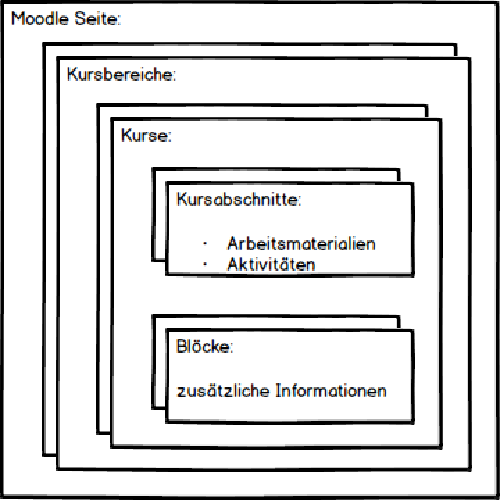
\includegraphics[width=.5\textwidth,center]{MoodleAufbau.pdf}
\caption{\label{fig:MoodleAufbau}Schematischer Aufbau einer Moodle Seite}
\end{figure}

\begin{figure}[h!]
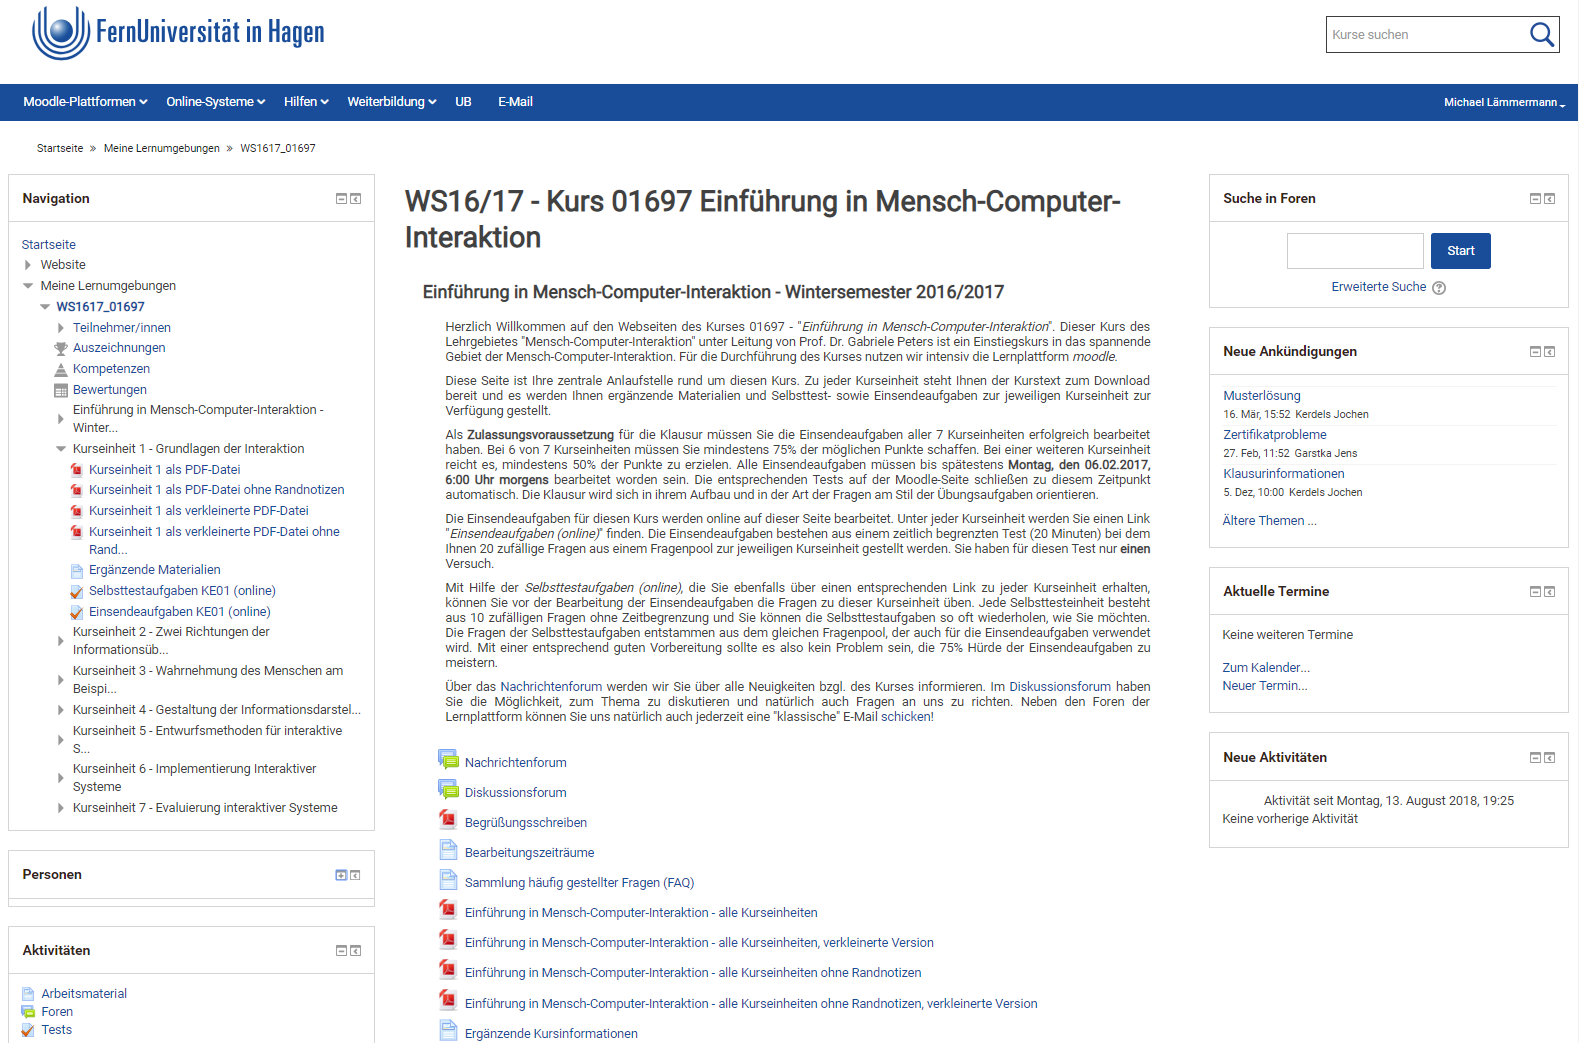
\includegraphics[width=\textwidth,center]{MoodleKursseitenbeispiel.png}
\caption{\label{fig:MoodleKursseitenbeispiel}Kursseite des Kurses \glqq Einführung in Mensch-Computer-Interaktion\grqq{} \citep{fernuniversitaet2018mensch}}
\end{figure}

%behauptung?
Technisch baut Moodle auf einem Aufbau aus Webserver und Datenbank unter Verwendung von PHP (PHP: Hypertext Preprocessor) auf. Um die zum Ziel gesetzte Personalisierbarkeit zu erreichen, setzt Moodle unter anderem auf ein Plugin-System. Plugins werden in über 50 verschiedene Plugin-Typen kategorisiert, wobei jeder dieser Typen dazu dient, einen speziellen Bereich von Moodle zu erweitern beziehungsweise anzupassen \citep{moodle2017plugin}.


%%%%%%%%%%
\section{Kooperation im Lernumfeld}
\glqq Lernen ist in vieler Hinsicht ein sozialer Prozess, der kulturelle Einflüsse einschließt sowie soziale Aktivitäten und gemeinsames Problemlösen umfasst\grqq{} \citep{reinmann1995kooperation}. %Diese Aussage macht die Bedeutung von Kooperation im Lernumfeld klar. 
%\textbf{Anhand dieser Aussage lässt sich schon grob erkennen, was unter Kooperation im Lernumfeld zu verstehen ist und welche Bedeutung dieser zugeordnet wird.}
Weitgefasst versteht man unter kooperativem Lernen eine Situation, in der zwei oder mehrere Personen zusammen lernen oder versuchen, zusammen zu lernen \citep{dillenbourg1999collaborative}.
%\todo[inline]{Verknüpfung}

Während in dieser Arbeit, wie im deutschsprachigen Raum üblich, keine Unterscheidung zwischen dem \textit{kooperativen} und dem \textit{kollaborativen} Lernen vorgenommen wird, werden die Begriffe außerhalb des deutschsprachigen Raums häufig differenziert betrachtet \citep{reinmann2002analyse}. Eine differenzierte Betrachtung der beiden Begriffe liefert \cite{dillenbourg1995evolution}. Demnach handelt es sich um \textit{Kooperation}, wenn eine Problemlösung durch die Arbeitsteilung unter den Mitgliedern einer Gruppe erreicht wird, wobei jedes Mitglied für einen Teil der Problemlösung verantwortlich ist.
Bei \textit{Kollaboration} wird die Problemlösung hingegen durch gemeinsames Engagement der Gruppenmitglieder bei koordiniertem Vorgehen zur Problemlösung erreicht.
Als Beispiel kann eine Gruppenarbeit mit der Aufgabe, mehrere Textabschnitte zusammenzufassen, betrachtet werden.
Bei einem kooperativen Vorgehen wäre zunächst jeweils ein Gruppenmitglied für die Zusammenfassung genau eines Textabschnittes verantwortlich. In einem zweiten Schritt würden dann die einzelnen Teilergebnisse zu einem Ergebnis zusammengefasst. Bei einem kollaborativen Vorgehen wiederum würden alle Gruppenmitglieder die einzelnen Textabschnitte gemeinsam zusammenfassen.

Dem kooperativen Lernen werden positive Effekt zugesprochen, unter anderem bezüglich der Lernmotivation \citep{reinmann1995kooperation,dillenbourg1999collaborative}. So wird beispielsweise beim Lernen durch Lehren, einer speziellen Form des kooperativen Lernens, die Motivation der Beteiligten erhöht. Gleichzeitig werden sowohl beim Lehrenden als auch beim Lernenden effektive Lernprozesse in Gang gesetzt \citep{reinmann1995kooperation}.

\cite{reinmann2002analyse} beschreiben auch, welche Probleme bei netzbasierten Umgebungen entstehen können. So können neben technischen Problemen auch Widerstände seitens der Nutzer vorliegen. Oftmals ist es schwer, die Gruppenmitglieder dazu zu bringen, aktiv an den netzbasierten Szenarien teilzunehmen. Auch besteht das Problem, dass in netzbasierten Umgebungen weniger individuelles als kollektives Wissen geteilt wird als in Face-to-Face-Situationen. Aufgrund der fehlenden sozialen Hinweisreize und der Anonymität kann \glqq es leicht zu unkontrollierter Kommunikation und heftigen Gefühlsausbrüchen, dem sog. Flaming, kommen\grqq{} \citep{reinmann2002analyse}.


%%%%%%%%%%
\section{Hypermedia}
Bevor mit der genauen Konzeption und Implementation des Hyperaudio-Plugins begonnen werden kann, werden \textit{Hypermedia} im Allgemeinen betrachtet. Dabei soll zunächst eine Begriffsklärung durchgeführt werden. Aus diversen Erfahrungen mit \textit{Hypermedia} können Rückschlüsse für das zu entwickelnde Moodle-Plugin und die zugrundeliegende Interpretation von \textit{Hyperaudio} gezogen werden.


%%%%%%%%%%
\subsection{Grundbegriffe}
Zu Beginn wird zunächst der Begriff \textit{Multimedia} betrachtet. Unter \textit{Multimedia} wird die Bereitstellung von Informationen mittels verschiedener Formate, beispielsweise Text, Audio, Bilder oder Video, bezeichnet \citep{mayer2009multimedia,moos2010multimedia}.

Der Begriff \textit{Hypermedia} wurde das erste Mal von Ted Nelson 1965 verwendet \citep{nelson1965complex}. In seinem Paper beschreibt er detailliert, was er sich unter einem \textit{Hypertext} vorstellt. Hierunter versteht er ein Dokument bestehend aus geschriebenen oder bildhaften Inhalten, welche in solch einer komplexen Art und Weise miteinander verbunden sind, dass sie nicht mehr auf Papier dargestellt werden können. Es kann Zusammenfassungen, Karten über die Inhalte und deren Zusammenhänge, Annotationen, Ergänzungen oder Anmerkungen von Wissenschaftlern, die das Dokument begutachtet haben, enthalten. Nelson beschreibt das Kriterium für den Präfix \textit{hyper} damit, dass diese Objekte nicht durch eine Konvertierung in ein einfaches lineares Medium, wie beispielsweise einen String umgewandelt werden können. Der wesentliche Punkt ist also, dass es sich beim Arbeiten mit \textit{Hypermedia} um ein nicht-lineares Vorgehen handelt.

Genauer betrachtet stellt das, was \cite{nelson1965complex} sich als \textit{Hypertext} vorgestellt hatte, nach \cite{nielsen2013multimedia} bereits eine Form von \textit{Hypermedia} dar. Auch wenn die beiden Begriffe \textit{Hypertext} und \textit{Hypermedia} synonym verwendet werden können, werden bei strikter Betrachtung bei \textit{Hypertext} ausschließlich Texte miteinander verbunden, während bei \textit{Hypermedia} auch andere Medien eingebunden werden können. Gemeinsam haben beide Arten jedoch, dass der Betrachter keinen linearen Weg vorgegeben hat, sondern von einem Knoten (Node) zum anderen springen kann und sich somit seinen Weg selbst aussucht. Demnach stellt \textit{Hypermedia} eine nicht-lineare Variante von \textit{Multimedia} dar.

Nach dieser Logik handelt es sich bei \textit{Hyperaudio} in seiner klassischen Form eigentlich um reine Audiosequenzen, die miteinander verknüpft sind, wobei der Zuhörer selbst entschieden kann, in welcher Reihenfolge er diese abspielt \citep{zumbach2006learning}.


%%%%%%%%%%
\subsection{Lernen mit Hypermedia}
Wissenschaftler beschäftigen sich schon seit vielen Jahren damit, festzustellen, welche Effekte der Einsatz von \textit{Multimedia}, \textit{Hypertext} und \textit{Hypermedia} auf den Lernerfolg von Lernenden hat.

%In der Arbeit von \cite{moos2010multimedia} wird eine Analyse von etlichen Arbeiten zu diesem Thema durchgeführt. \cite{moos2010multimedia} konzentrieren sich hierbei vor allem auf den Einfluss auf die Motivation der Lernenden. Dennoch wird auch auf andere Aspekte der drei verschiedenen E-Learning Methoden \textit{Multimedia}, \textit{Hypertext} und  \textit{Hypermedia} im Vergleich zu klassischen Lehrmethoden eingegangen.

\cite{mayer2009multimedia} konnte am Ende seiner Untersuchungen positive Effekte beim Einsatz von \textit{Multimedia} nachweisen. So schnitten Studenten bei einem Transfertest besser ab, wenn sie mit Text und Bildern lernten, als wenn sie ausschließlich mit Text lernten. \cite{mayer2009multimedia} knüpft dieses Ergebnis aber an folgende Prinzipien, welche beim Einsatz von \textit{Multimedia} befolgt werden müssen:

\begin{itemize}
 \item  Kohärenz: irrelevante Wörter, Töne und Bilder sollten vermieden werden
 \item	Signalisieren: essentielle Inhalte sollten hervorgehoben sein
 \item	Redundanz: Text sollte ausschließlich auditiv statt auditiv und visuell in Multimediapräsentationen wiedergegeben werden
 \item	Räumliche Nähe: zusammengehörige Texte und Bilder sollten nah beieinander statt weit entfernt auf der Seite beziehungsweise dem Bildschirm dargestellt werden
 \item	Zeitliche Nähe: zusammengehörige Texte und Bilder sollten gleichzeitig statt nacheinander auf der Seite beziehungsweise dem dargestellt werden
 \item	Segmentierung: temporeiche, komplexe Multimedia–Lektionen sollten in benutzerfreundlichen Stücken statt im Ganzen präsentiert werden
 \item	Vorbereitung: der Lernende sollte die Begrifflichkeiten und Merkmale der Lektion kennen
 \item	Modalität: Text sollte auditiv statt visuell wiedergegeben werden
 \item	Personalisierung: Texte sollten in dialogorientiertem Stil statt in formellem Stil wiedergegeben werden
 \item	Stimme: Text sollte von einer freundliche menschlichen Stimme statt einer Computerstimme wiedergegeben werden
\end{itemize}


Im Gegenzug verweisen \cite{moos2010multimedia} auf Arbeiten, nach denen eine Herausforderung bei \textit{Multimedia} und somit auch bei \textit{Hypermedia} darin besteht, dass die kognitive Aufnahmekapazität der Studierenden überschritten werden kann, wenn Informationen sowohl aus einem Text als auch aus einem Diagramm entnommen werden sollen (Mayer und Moreno; van Merrienboer und Ayres, nach \cite{moos2010multimedia}). Dies beruht auf der Annahme der Cognitive Load Theory, welche dem Arbeitsgedächtnis nur eine begrenzte Kapazität zuspricht (Sweller; van Merrienboer und Sweller, nach \cite{moos2010multimedia}).

\textit{Hypertext} bietet zwar Vorteile, da der Studierende den Lernweg bestimmen kann, der am besten auf seine Bedürfnisse angepasst ist. Auf der anderen Seite ist hierzu aber eine ausreichende Vorkenntnis in dem entsprechenden Lernbereich notwendig, um die Entscheidung treffen zu können, wie dieser Weg aussehen soll. Des Weiteren wirkt sich auch ein fehlendes Interesse des Studierenden negativ auf die Effektivität der \textit{Hypertext}-Lernumgebung aus (Lawless und Kulikowich, nach \cite{moos2010multimedia}).

Es ist nun also nicht verwunderlich, dass \textit{Hypermedia} als Verschmelzung von \textit{Multimedia} und \textit{Hypertext} ebenfalls einige Herausforderungen mit sich bringt \citep{moos2010multimedia}. Scott und Schwartz (nach \cite{moos2010multimedia}) fordern für das Lernen mit \textit{Hypermedia} eine Balance zwischen effektiver Navigation und Inhaltsverständnis. Dies soll durch Prozesse zur Überwachung des eigenen Lernfortschritts erreicht werden, doch Untersuchungen haben ergeben, dass viele Studierende Schwierigkeiten dabei haben, diese Prozesse korrekt anzuwenden \citep{moos2010multimedia}.

\label{sec:audiocues}
\cite{donker2007gestaltung} weisen auf die Probleme bei der Verwendung von \textit{Hyperaudio} hin. Hier besteht die Herausforderung darin, dem Hörer die Hyperlinks innerhalb einer \textit{Hyperaudio}-Anwendung sinnvoll darzustellen. Bei ihrer Untersuchung kamen \cite{donker2007gestaltung} zu dem Ergebnis, \glqq dass sowohl eine Verdeutlichung
von Links durch das Voranstellen eines Tons als auch die Variante durch das
Ändern des Alters des Sprechers zu guten Ergebnissen hinsichtlich des Erkennens des Links
führen.\grqq{} Die genannten vorangestellten Töne werden auch als \textit{Audio Cues} bezeichnet.

\subsection{Repräsentation von Kurseinheiten im Hyperaudio-Format}
\label{sec:hyperaudio}

Nachdem nun die Begrifflichkeiten um \textit{Hypermedia}, sowie den Begriff \textit{Hyperaudio} im eigentlichen Sinne beleuchtet und entsprechende Studien betrachtet wurden, wird nun darauf eingegangen, welche Rückschlüsse daraus für diese Arbeit gezogen werden können.

Um eine auditive Repräsentation der Kurseinheiten umsetzen zu können, müssen deren Inhalte entsprechend auditiv aufbereitet werden. Inhalte, die nicht auditiv umgesetzt werden können, können in visueller Darstellung zum entsprechenden Zeitpunkt an den Audioinhalt annotiert werden.

In Ergänzung zu \cite{zumbach2006learning} wird in dieser Arbeit unter \textit{Hyperaudio} ein Audioinhalt verstanden, der mittels der Erweiterung durch Kommunikations- und Interaktionsmöglichkeiten (vgl. Abschnitt \ref{sec:zielsetzung}) sowie visuelle Inhalte um Multimedia- und Hypermedia-Elemente ergänzt wird. Ein Hyperaudio-Dokument im Sinne dieser Arbeit besteht aus auditiven Inhalten und annotierten visuellen Inhalten. Bei den Hyperaudio-Dokumenten handelt es sich somit eigentlich um Multimedia-Dokumente. Erst die Kommunikations- und Interaktionsmöglichkeiten führen dazu, dass der \textit{Hypermedia}-Aspekt erfüllt wird. 

Der Vorteil dieser Betrachtungsweise von \textit{Hyperaudio} liegt darin, dass die Herausforderungen, die in Verbindung mit \textit{Hypermedia} bzw. \textit{Hypertext} normalerweise auftreten, nicht besonders prägnant sind. Im zu entwickelnden Moodle-Plugin wird dem Studierenden in erster Linie ein linearer Audioinhalt vorgespielt, der um Multimedia-Elemente ergänzt wird. Erst durch den Einsatz der Kommunikations- und Interaktionsmöglichkeiten kommen die herausfordernden Elemente von \textit{Hypermedia} ins Spiel. Dementsprechend stellt das Hyperaudio-Plugin einen guten Kompromiss zwischen den verschiedenen Lehrmethoden dar.


%%%%%%%%%%
\section{Zusammenfassung}
%Zu Beginn dieses Kapitels wurde zunächst auf Medien und deren Effekte eingegangen, um vorab auf die möglichen Effekte der Einführung der Hyperaudio-Lernumgebung als neues Medium hinzuweisen. Darauf folgend wurde ein Überblick über die Lernplattform Moodle gegeben, um eine besseres Verständnis für Moodle im Laufe dieser Arbeit zu schaffen. Im nächsten Schritt wurde der Begriff der Kooperation im Lernumfeld, dessen generelle Vorteile sowie dessen Probleme in netzbasierten Umgebungen beleuchte Dies soll dazu dienen die Bedeutung der Kommunikation und der damit verbunden Probleme für das Hyperaudio-Plugin aufzuzeigen. Um ein grundlegendes Verständnis für die Begrifflichkeit \textit{Hyperaudio} zu schaffen, wurden die Begriffe \textit{Multimedia}, \textit{Hypermedia}, \textit{Hypertext} sowie \textit{Hyperaudio} selbst erläutert und deren Vor- und Nachteile anhand vorhandenen Studien dargelegt. Abschließend wurde darauf basierend festgelegt in wie \textit{Hyperaudio} bei der Repräsentation von Kurseinheiten im Hyperaudio-Format zu verstehen und einzusetzen ist.
%
%\todo[inline]{Korrigieren}
\todo[inline]{Zusammenfassung schreiben}


%%%%%%%%%%%%%%%%
\chapter{Analyse}
%% lade Kapitel aus Datei
\label{cha:analyse}
Für die Konzeption und Implementierung des Hyperaudio"=Plugins ist zunächst eine Analyse notwendig. Basierend auf einer Zielgruppenanalyse sollen Anforderungen an das Plugin bestimmt und priorisiert werden. Darauf aufbauend werden Möglichkeiten und Technologien zur Umsetzung des Hyperaudio"=Plugins begutachtet.

%\begin{figure}[h!]
%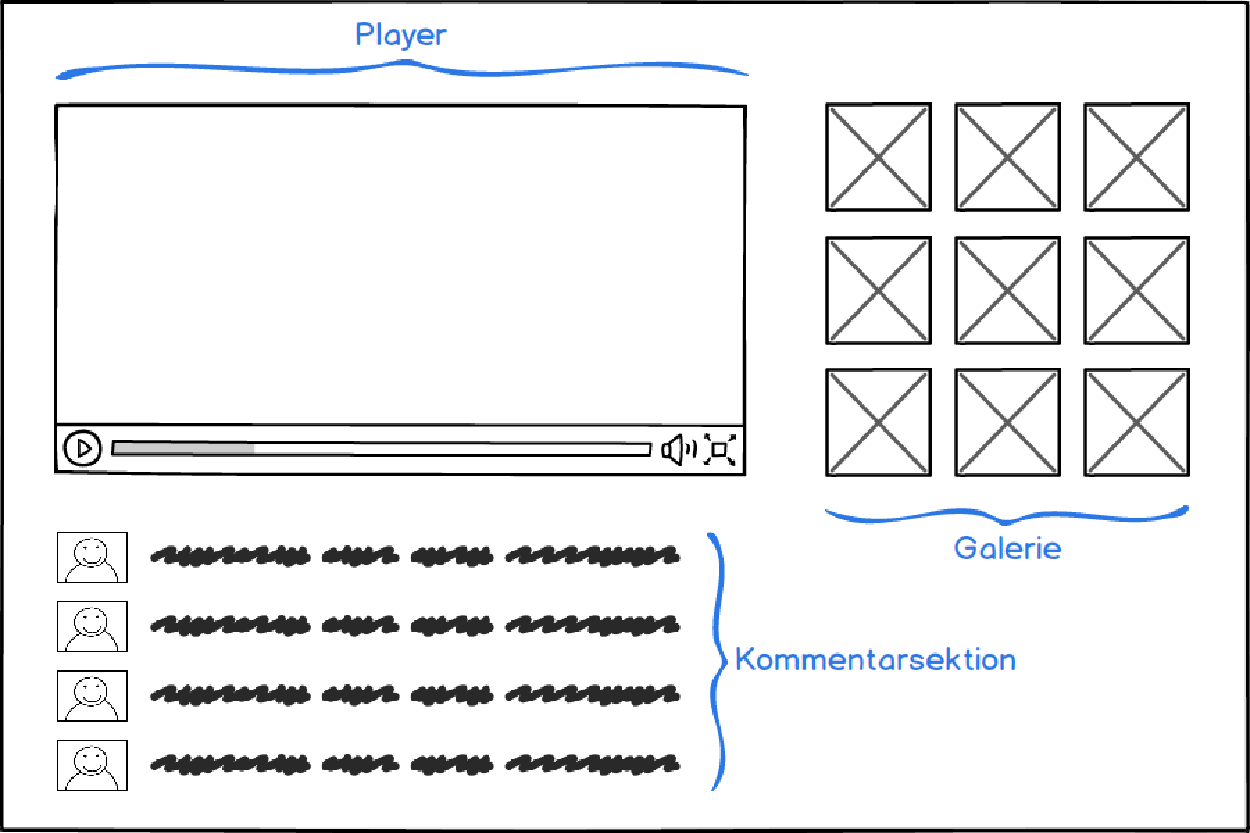
\includegraphics[width=.8\textwidth,center]{MockupBereiche.pdf}
%\caption{\label{fig:MockupBereiche}Erste Skizze der Moodle-Repräsentation eines Hyperaudio-Dokuments}
%\end{figure}


%%%%%%%%%%
\section{Zielgruppe}
Im ersten Schritt soll die Zielgruppe anhand von \textit{Personas} und deren \textit{User Stories} festgelegt werden. Diese sollen dann die Grundlage für die Definition der Anforderungen im nächsten Abschnitt darstellen.


%%%%%%%%%%
\subsection{Personas}
\label{sec:personas}
%https://dl.gi.de/bitstream/handle/20.500.12116/5888/Holt_Winter_Thomaschewski_2011.pdf?sequence=2
Unter \textit{Personas} werden fiktive Benutzer verstanden, für welche das Programm, in unserem Fall das Moodle-Plugin, designt wird \citep{cooper2004inmates}. Jeder Persona wird eine Rolle im Zusammenhang mit der Anwendung zugewiesen. Darüber hinaus wird die Persona ausreichend beschrieben, damit sich leicht in die Person hineinversetzt werden kann \citep{cohn2004user}. Dieses Vorgehen hilft dabei, möglichst authentische \textit{User Stories} zu generieren, ohne auf echte Benutzer zurückgreifen zu müssen. Darüber hinaus ist festzustellen, dass die realen Anwender zwar Problemstellungen identifizieren können, aber nicht unbedingt in der Lage sind, Anforderungen zur Lösung dieser Probleme zu formulieren \citep{cooper2004inmates}. Für die Analyse und Konzeption des Hyperaudio"=Plugins wird mit folgenden Personas gearbeitet:

\par
\begingroup
\leftskip=1cm
\rightskip=1.5cm
\noindent

{\Large\emph{Prof. Dr. Karolin Schröder}} ist verantwortlich für den Kurs \glqq Einführung in die Wirtschaftsinformatik\grqq{}. In diesem Kurs werden bereits erfolgreich Hyperaudio-Dokumente eingesetzt. Nachdem Prof. Dr. Schröder mit dem Start des nächsten Semesters überarbeitete Kurseinheiten anbietet, müssen nun auch die zugehörigen Hyperaudio-Dokumente auf die Notwendigkeit einer Überarbeitung hin überprüft werden. Die veralteten Hyperaudio-Dokumente müssen dann durch neuere Versionen ersetzt werden.
\vspace{.5cm}

{\Large\emph{Dr. Julian Schmidt}} ist wissenschaftlicher Mitarbeiter und Betreuer für den Kurs \glqq Marketing\grqq{}, der ebenfalls das Lernen mittels Hyperaudio-Dokument anbietet. Dr. Julian Schmidt ist unter anderem für die Betreuung dieser verantwortlich und ist derjenige, der hier Rede und Antwort steht.
\vspace{.5cm}

{\Large\emph{Laura Ebert}} ist 35 Jahre alt, verheiratet und hat drei Kinder. Sie geht halbtags ihrem Beruf als Anwendungsentwicklerin nach, zu dem sie 30 Minuten mit dem Bus pendelt. Neben der Arbeit kümmert sie sich zusammen mit ihrem Mann um den Haushalt und die Kinder. Laura studiert in Teilzeit den Bachelorstudiengang Informatik im ersten Semester. Das Semester hat erst vor einigen Wochen begonnen und sie entdeckt gerade Moodle für sich. Hierbei ist sie auf die Hyperaudio-Dokumente gestoßen und hat sich fest vorgenommen, sich im Laufe des Semsters mit deren Hilfe mit den Lerninhalten auseinanderzusetzen.
\vspace{.5cm}
 
{\Large\emph{Max Lustig}} ist 24 Jahre alt, ledig und hat sich nach einer abgeschlossenen Ausbildung zum Informatikkaufmann dazu entschlossen, neben dem Beruf zu studieren. Zur Arbeit kommt er in wenigen Minuten zu Fuß. Viel Zeit verbringt er jedoch im Fitnesstudio mit Kraft- und Ausdauertraining. Er absolviert ein Vollzeitbachelorstudium der Wirtschaftsinformatik und befindet sich kurz vor der Prüfungsphase zum Ende des dritten Semesters. Max möchte sich nun auf die Klausur des Moduls \glqq Investition und Finanzierung (BWL II)\grqq{}, welche in zwei Wochen stattfindet, intensiv vorbereiten. Im Laufe des Semsters hat er bereits ausgiebig die neuen Hyperaudio-Dokumente zum Erreichen des Lernziels genutzt.

\par
\endgroup

%%%%%%%%%%
\subsection{User Stories}
\label{sec:UserStories}
Unter Zuhilfenahme der entwickelten Personas werden im nächsten Schritt \textit{User Stories} formuliert. \textit{User Stories} beschreiben, wie die klassischen \textit{Use Cases}, Anforderungen an ein Softwaresystem. Sie sind dabei im Vergleich wesentlich oberflächlicher und ungenauer formuliert als \textit{Use Cases} \citep{wirdemann2017scrum}. Erst im Laufe der Entwicklung werden \textit{User Stories} konkreter und dienen am Ende dazu, das Entwicklungsergebnis zu validieren. Beim Erstellen von \textit{User Stories} ist zu beachten, dass sogenannte \textit{Epics}, das sind \textit{User Stories} mit sehr großem Umfang, wenn möglich in kleinere \textit{User Stories} aufgesplittet werden. Unter anderem ist zu beachten, dass die \textit{User Stories} keine Abhängigkeiten untereinander aufweisen und dass deren Erfüllung überprüfbar ist. \textit{User Stories} können im \textit{Connextra Format} festgehalten werden, welches wie folgt aufgebaut ist \citep{cohn2004user}:

\par
\begingroup
\leftskip=1cm
\rightskip=1.5cm
\noindent

\textit{Ich als (Rolle) möchte (Funktion), um (Nutzen).}

\par
\endgroup

\vspace{.3cm}

Mit den Unterschieden und Einsatzzwecken von Personas und Rollen beschäftigt sich \cite{constantine2006users}. Grundsätzlich ist demnach festzustellen, dass Personas eher aus dem \textit{User-centered design} \citep{Norman1986user}, Benutzerrollen dagegen aus dem \textit{Usage-centered design} \citep{Constantine1996usage} motiviert sind. Während sowohl Personas als auch Benutzerrollen durchaus nützlich sind, um ein Verständnis von den Nutzern eines Systems zu erhalten, unterscheiden sie sich nach \cite{constantine2006users} in ihrer Philosophie und Relevanz für das Interaktionsdesign. Im Gegensatz zu Personas, die wie bereits im vorangegangenen Abschnitt \ref{sec:personas} beschrieben dazu dienen, die Nutzersicht anhand möglichst realer Personen darzustellen, sollen Benutzerrollen in einer wesentlich technischeren Sicht ein abstrahiertes Modell für die Art und Weise, in der Nutzer mit dem System interagieren, bilden \citep{constantine2006users}.

Für die weitere Analyse soll das Beste beider Welten vereinbart werden. Um die User Stories möglichst anschaulich zu halten, werden sie anhand der vorgestellten Personas definiert. Gleichzeitig wird eine Aufteilung in Benutzerrollen vorgenommen, welche die Grundlage für die Ableitung von Anforderungen aus den User Stories bilden soll.

Für die Konzeption des Hyperaudio"=Plugins ergeben sich im Wesentlichen zwei Benutzerrollen wie in Abbildung \ref{fig:Rollen} dargestellt. \textit{Administrierende} sind diejenigen Anwender, die Lerninhalte in Form von Hyperaudio-Dokumenten bereitstellen und verwalten. Diese Rolle kann nur von Lehrenden eingenommen werden. Die Gruppe der \textit{Nutzenden} kann derweil aus Lehrenden sowie Studierenden bestehen, die mit Hyperaudio-Dokumenten interagieren möchten.

\begin{figure}[h!]
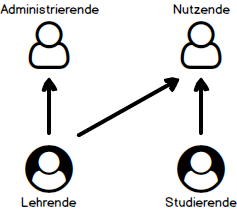
\includegraphics[width=.3\textwidth,center]{Rollen.png}
\caption{\label{fig:Rollen}Benutzerrollen}
\end{figure}

\FloatBarrier

Für das Angebot einer Hyperaudio-Lernumgebung lassen sich folgende User Stories festhalten:

\begin{enumerate}[leftmargin=1.3cm,label=US-\arabic*:,ref=US-\arabic*]

\item \label{US-Admin-Erstellen} Als Administrierende möchte Prof. Dr. Karolin Schröder ein neues Hyperaudio"=Dokument in ihrem Kurs \glqq Einführung in die Wirtschaftsinformatik\grqq{} zur Verfügung stellen, um den Studierenden neue Lerninhalte bereitzustellen.

\item \label{US-Admin-Loeschen} Als Administrierende möchte Prof. Dr. Karolin Schröder Hyperaudio"=Dokumente aus ihrem Kurs \glqq Einführung in die Wirtschaftsinformatik\grqq{} löschen können, um veraltete Informationen zu entfernen.

\item \label{US-Admin-Semester} Als Administrierende möchte Prof. Dr. Karolin Schröder Hyperaudio"=Dokumente aus ihrem Kurs \glqq Einführung in die Wirtschaftsinformatik\grqq{} im Sommersemester in den darauffolgenden Kurs im Wintersemester übernehmen, um diese nicht erneut erstellen zu müssen.

\item \label{US-Admin-Kurs} Als Administrierende möchte Prof. Dr. Karolin Schröder Hyperaudio"=Dokumente anderer Kurse in ihren Kurs \glqq Einführung in die Wirtschaftsinformatik\grqq{} übernehmen, um auf die hervorragende Arbeit anderer Lehrender zurückgreifen zu können, da sich die Themen mit ihrem Kurs überschneiden.

\item \label{US-Admin-Statistik} Als Administrierende möchte Prof. Dr. Karolin Schröder Erkenntnisse daraus gewinnen, wie die Hyperaudio"=Dokumente des Kurses \glqq Einführung in die Wirtschaftsinformatik\grqq{} von Studierenden genutzt werden, um Verbesserungspotenzial auszumachen.

\item \label{US-Admin-Bearbeiten} Als Administrierender möchte Dr. Julian Schmidt ein vorhandenes Hyperaudio"=Dokument in dem von ihm betreuten Kurs \glqq Marketing\grqq{} überarbeiten, um einen Fehler zu beseitigen.

\item \label{US-Wiedergabe} Als Nutzende möchte Prof. Dr. Karolin Schröder die bereits vorhandenen Hyperaudio"=Dokumente aus ihrem Kurs \glqq Einführung in die Wirtschaftsinformatik\grqq{} wiedergeben, um diese auf ihre Richtigkeit zu überprüfen.

\item \label{US-Antwort-L} Als Nutzende möchte Prof. Dr. Karolin Schröder die Kommentare zu einem Hyperaudio"=Dokument lesen und beantworten können, um auf Fragen von Studierenden einzugehen.

\item \label{US-Notiz-L} Als Nutzende möchte Prof. Dr. Karolin Schröder eine Notiz zu einem Hyperaudio"=Dokument machen, um ihren Gedanken festzuhalten und später darauf zurückgreifen zu können.

\item \label{US-Kommentar-L} Als Nutzender möchte Dr. Julian Schmidt eine gefundene Erklärungslücke in einem Hyperaudio"=Dokument durch einen Kommentar zum entsprechenden Zeitpunkt schließen, um eventuellen Fragen der Studierenden zuvorzukommen.

%\item \textit{Dr. Julian Schmidt stellt eine Erklärungslücke in einem Hyperaudio"=Dokument fest und möchte diese durch einen Kommentar zum entsprechenden Zeitpunkt schließen.}

\item \label{US-Zeit} Als Nutzende möchte Laura Ebert mittels Hyperaudio"=Dokument lernen, um die Zeit während Haushaltsarbeiten, wie dem Bügeln, Kochen oder Putzen, und dem Pendeln sinnvoller zu nutzen.

\item \label{US-Uebersicht-Kurse} Als Nutzende möchte Laura Ebert erfahren, welche Hyperaudio"=Dokumente in den von ihr belegten Kursen angeboten werden, um herauszufinden, mit welchen Mitteln sie sich auf die anstehenden Prüfungen vorbereiten kann.

\item \label{US-Kommentar-S} Als Nutzende möchte Laura Ebert einen Kommentar verfassen, um dem Kursbetreuer und den anderen Studierenden eine Frage zu stellen.

\item \label{US-Lesezeichen} Als Nutzende möchte Laura Ebert ein Lesezeichen setzen, wenn eine klausurrelevante Thematik erklärt wird. Bei der Prüfungsvorbereitung möchte sie anhand dieser Lesezeichen diejenigen Themen erkennen, mit welchen sie sich besonders intensiv beschäftigen möchte.

\item \label{US-Lesezeichen-Loeschen} Als Nutzende möchte Laura Ebert ein Lesezeichen löschen, da sie den markierten Lerninhalt inzwischen beherrscht. Anhand der übrigen Lesezeichen möchte sie schnell erkennen, wo für sie noch Lernbedarf besteht.

\item \label{US-Notiz-S} Als Nutzende möchte Laura Ebert eine Notiz erstellen, um ein Beispiel zu dem genannten Sachverhalt festzuhalten, sodass sie die Thematik beim nächsten Mal einfacher nachvollziehen kann.

\item \label{US-Fortsetzen} Als Nutzende möchte Laura Ebert die Wiedergabe eines Hyperaudio"=Dokuments beenden und am nächsten Tag automatisch an derselben Stelle fortsetzen können, um das Lernen schnell wiederaufnehmen zu können.

\item \label{US-Mobil} Als Nutzende möchte Laura Ebert die Hyperaudio-Angebote mit ihrem Smartphone in Anspruch nehmen, um auch die Zeit während des Pendelns zum Lernen nutzen zu können.

\item \label{US-Notiz-Bearbeiten} Als Nutzender möchte Max Lustig eine alte Notiz bearbeiten, um einen Schreibfehler zu korrigieren.

\item \label{US-Notiz-Loeschen} Als Nutzender möchte Max Lustig eine alte Notiz löschen, da er inzwischen Lernfortschritte gemacht hat und auf diese Notiz verzichten kann.

\item \label{US-Galerie} Als Nutzender möchte Max Lustig schnell erkennen welche Inhalte im Hyperaudio"=Dokument behandelt werden, um eine Erklärung eines bestimmten Themas zu finden.

\item \label{US-Suche} Als Nutzender möchte Max Lustig nach Textinhalten in Kommentaren suchen können, um schnell Erklärungen zu finden.

\item \label{US-Sortierung-Erstellungsdatum} Als Nutzender möchte Max Lustig die Kommentare nach Erstellungsdatum sortieren können, um sich einen Überblick über die neuesten Aktionen zu verschaffen.

\item \label{US-Sortierung-Zeitpunkt} Als Nutzender möchte Max Lustig die Kommentare und persönlichen Notizen zu den Annotationszeitpunkten zuordnen können, um diese bei der Wiedergabe verfolgen zu können.

\item \label{US-Filter} Als Nutzender möchte Max Lustig öffentliche Kommentare und persönliche Notizen getrennt betrachten können, um die öffentliche Diskussion verfolgen beziehungsweise die eigenen Anmerkungen isoliert betrachten zu können.

\item \label{US-Antwort-S} Als Nutzender möchte Max Lustig auf Kommentare antworten können, um sich mit den Studierenden und Lehrenden auszutauschen.

\item \label{US-Uebersicht-Letzte} Als Nutzender möchte Max Lustig erkennen, welche Hyperaudio"=Dokumente er zuletzt abgespielt hat, um seinen Lernfortschritt im Auge zu behalten.

\item \label{US-Favoriten} Als Nutzender möchte Max Lustig besonders hilfreiche Hyperaudio"=Dokumente als Favoriten speichern, um diese schnell als solche identifizieren zu können.

\item \label{US-Favoriten-Loeschen} Als Nutzender möchte Max Lustig die Markierung als Favorit entfernen können, wenn der Inhalt für ihn nicht mehr von Interesse ist.

\item \label{US-Zeit-Mobil} Als Nutzender möchte Max Lustig auf seinem Tablet Zugang zu Hyperaudio"=Dokumenten haben, um die Zeit auf dem Laufband gleichzeitig zum Lernen nutzen zu können.

\end{enumerate}

Natürlich könnten noch mehr User Stories formuliert werden. Die 30 genannten User Stories sollen jedoch für diese Arbeit die Basis der Anforderungsdefinition bilden. Auch die Evaluation des Entwicklungsergebnisses soll anhand der User Stories durchgeführt werden.

%%%%%%%%%%
%\subsection{Umgebungsbedingungen}
%Aus den in Abschnitt \ref{sec:personas} beschriebenen \textit{Personas} und den in Abschnitt \ref{sec:UserStories} beschriebenen \textit{User Stories} können die Umgebungsbedingungen des \textit{Hyperaudio}-Plugins abgelesen werden. Diese stellen den Rahmen dar, in dem das Plugin durch die Studierenden genutzt werden können soll und spiegeln teilweise bereits Anforderungen wieder.
%
%So ergeben sich folgende Umgebungsbedingungen:
%
%\begin{itemize}
%\item Möglichkeit zur Nutzung des Plugins während der Ausübung anderer Tätigkeiten (Hausarbeit, Sport, Pendeln etc.)
%\item Unterstützung von verschiedenen Endgeräten (Desktop/Laptop, Tablet, Smartphone  etc.)
%\end{itemize}
%
%
%\todo[inline]{Rahmen in dem das Plugin durch Studierende genutzt werden können soll}
%- Während unbezahlter Arbeit
%- Beim Sport
%- An mobilen Endgeräten


%%%%%%%%%%
\section{Anforderungsdefinition}
\label{sec:anforderungsdefinition}
Basierend auf den Personas, Rollen und User Stories können nun die Anforderungen für das Hyperaudio"=Plugin definiert werden. Hierbei werden aus einer oder mehreren User Stories jeweils eine oder mehrere Anforderungen abgeleitet und zugleich mit einer Priorität versehen. Für die Priorisierung stehen die drei Prioritätsstufen \textit{niedrig}, \textit{mittel} und \textit{hoch} zur Verfügung. Während im Rahmen eines partizipativen Entwicklungsansatzes eine Bewertung der User Stroies oder Anforderungen durch zukünftige Nutzer in Betracht gezogen werden kann, soll in dieser Arbeit die Zielsetzung aus Kapitel \ref{cha:einfuehrung} als Orientierung für die Priorisierung der Anforderungen dienen.

%%%%%%%%%%
\subsection{Anforderungen der Administrierenden}
\label{sub:AnforderungenDerAdministrierenden}
Es wird mit der Definition der Anforderungen der Administrierenden begonnen, welche in Tabelle \ref{tab:AnforderungenAdministrierenden} festgehalten werden. 

Aus \ref{US-Admin-Erstellen} kann die Anforderung des Erstellens von Hyperaudio"=Dokumenten abgeleitet werden. Dass bestehende Hyperaudio"=Dokumente auch bearbeitet und gelöscht werden können sollen, ergibt sich aus \ref{US-Admin-Bearbeiten} und \ref{US-Admin-Loeschen}. Zusammen stellen diese Anforderungen die Grundfunktionalitäten für die alternative Repräsentation der Lerninhalte dar und werden dementsprechend mit der Prioritätsstufe \textit{hoch} versehen.

Aus \ref{US-Admin-Semester} und \ref{US-Admin-Kurs} ergibt sich die Anforderung, dass Hyperaudio"=Dokumente in einen anderen Kurs übernommen werden können sollen, sei es der gleiche Kurs im nächsten Semester oder ein anderer Kurs. Diese Anforderung zählt nicht zu den Grundfunktionalitäten, kann das Verwalten von Hyperaudio"=Dokumenten jedoch vereinfachen und wird daher mit der Prioritätsstufe \textit{mittel} bewertet.

Der Wunsch, Erkenntnisse aus der Nutzung von Hyperaudio"=Dokumenten durch die Studierenden zu erhalten (\ref{US-Admin-Statistik}), schlägt sich in der Anforderung nach statistischen Auswertungsmöglichkeiten nieder. Für diese Anforderung wird die Priorität \textit{niedrig} vergeben, da es sich um ergänzende Metainformationen handelt.


\begin{table}[!ht]
\def\arraystretch{1.4}

 \begin{tabularx}{\textwidth}{lXc}      
    \hline
    Nr. & Anforderung & Priorität
    \\\hline
    1 & Erstellen eines Hyperaudio"=Dokuments & hoch\\
    2 & Bearbeiten eines Hyperaudio"=Dokuments & hoch\\
    3 & Löschen eines Hyperaudio"=Dokuments & hoch\\
    4 & Übernahme eines Hyperaudio"=Dokuments in einen anderen Kurs & mittel\\
    5 & Statistische Auswertungen über die Nutzung der Hyperaudio"=Dokumente & niedrig\\
    \hline
    \end{tabularx}
    \caption{Anforderungen von Administrierenden}
\label{tab:AnforderungenAdministrierenden}
\end{table}

%%%%%%%%%%
\subsection{Anforderungen der Nutzenden}
\label{sub:AnforderungenDerNutzenden}
Die aus den User Stories der Nutzenden abgeleiteten Anforderungen sind in Tabelle \ref{tab:AnforderungenNutzenden} festgehalten. Die Priorisierung wird dabei nach folgenden Kriterien vorgenommen:

\begin{itemize}
\item \textit{hoch}: Basisfunktionalität zum Erreichen der Zielsetzung der Arbeit
\item \textit{mittel}: Verbesserung der Interaktion mit Hyperaudio"=Dokumenten und Annotationen
\item \textit{niedrig}: Vereinfachter Zugriff auf Hyperaudio"=Dokumente
\end{itemize}


Aus \ref{US-Wiedergabe}, \ref{US-Zeit}, \ref{US-Mobil} und \ref{US-Zeit-Mobil} ergibt sich die grundlegende Anforderung, Hyperaudio"=Dokumente abspielen zu können. \ref{US-Zeit}, \ref{US-Mobil} und \ref{US-Zeit-Mobil} führen zudem zur Anforderung der Audio Cues, mithilfe derer auf annotierte Zusatzinhalte\footnote{Zusatzinhalte sind die nicht in auditiver Form repräsentierbaren Inhalte von Kurseinheiten.} hingewiesen wird. Diese Audio Cues wären zwar auch für Kommentare, Notizen oder Lesezeichen denkbar, doch würde dies selbst bei Verwendung verschiedener Audio Cues dazu führen, dass der Studierende mit unnötigen Informationen (im Sinne des zu vermittelnden Lerninhaltes) überhäuft würde. Dies widerspräche jedoch Mayers Prinzipien für Multimedia \citep{mayer2009multimedia}. Die Audio Cues für Zusatzinhalte können zu den Basisfunktionalitäten des Hyperaudio"=Plugins gezählt werden, da erst dadurch das Ziel der größeren zeitlichen Flexibilität beim Lernen erreichbar wird (vgl. Abschnitte \ref{sec:zielsetzung} und \ref{sec:audiocues}). Um Inhalte schnell auffinden zu können, wie in \ref{US-Galerie} gefordert, ist zudem eine Übersicht über annotierte Zusatzinhalte nützlich.

Basierend auf \ref{US-Antwort-L}, \ref{US-Kommentar-L}, \ref{US-Kommentar-S}, \ref{US-Sortierung-Zeitpunkt} und \ref{US-Antwort-S} lässt sich die Anforderung an eine Kommentarfunktion ableiten, die über Möglichkeiten zum Erstellen, Anzeigen und Beantworten von Kommentaren verfügen muss. An dieser Stelle kann die Interaktion durch eine Suchfunktion innerhalb der Kommentare verbessert werden (vgl. \ref{US-Suche}). In den \textit{User Stories} \ref{US-Notiz-L}, \ref{US-Notiz-S}, \ref{US-Notiz-Bearbeiten}, \ref{US-Notiz-Loeschen} und \ref{US-Sortierung-Zeitpunkt} werden Wünsche bezüglich einer Notizfunktion formuliert. Diese lässt sich aufschlüsseln in die Anforderungen zum Erstellen, Anzeigen, Bearbeiten und Löschen von Notizen. Die Notizfunktion spiegelt das Ziel der Erhaltung typischer Nutzerinteraktionen mit textuellen Lernmedien wieder und kann das Lernen für die Studierenden erleichtern \citep{scutter2010students}. Ähnlich sind die Anforderung zum Erstellen, Anzeigen und Löschen von Lesezeichen aus \ref{US-Lesezeichen} und \ref{US-Lesezeichen-Loeschen} zu bewerten. Obwohl Lesezeichen, ebenso wie die Notizfunktion, zu den Basisfunktionalitäten des Plugins gezählt werden können, wird die Lesezeichenfunktion mit der Priorität \textit{mittel} versehen. Das Herabsetzen der Priorität wird dadurch begründet, dass ein Lesezeichen im Wesentlichen einer Notiz ohne textuellen Inhalt entspricht und durch die höher priorisierte Notizfunktion abgebildet werden kann. Aus \ref{US-Sortierung-Erstellungsdatum}, \ref{US-Sortierung-Zeitpunkt} und \ref{US-Filter} ergibt sich zudem der Wunsch nach Filter- und Sortiermöglichkeiten. 

Der Wunsch nach einer Favoritenfunktion für Hyperaudio"=Dokumente ergibt sich aus \ref{US-Favoriten} und \ref{US-Favoriten-Loeschen}. Daraus resultieren die Anforderungen, Favoriten zu setzen, anzuzeigen und zu löschen. Übersichten über Hyperaudio"=Dokumente werden in \ref{US-Uebersicht-Kurse} und \ref{US-Uebersicht-Letzte} gefordert: im ersten Fall eine Übersicht über alle Hyperaudio"=Dokumente der belegten Kurse und im zweiten Fall eine Übersicht über die zuletzt abgespielten Hyperaudio"=Dokumente. Sowohl die Favoritenfunktion als auch die Übersichten stellen eine reine Optimierung der Navigation dar und verhelfen somit zu einem vereinfachten Zugriff auf Hyperaudio"=Dokumente. \ref{US-Fortsetzen} bringt die Anforderung für eine Funktion zum Fortsetzen unterbrochener Wiedergaben bei folgenden Aufrufen in Moodle hervor. Auch diese Funktion vereinfacht die Navigation zum gewünschten Hyperaudio"=Dokument beziehungsweise dessen Inhalt.

Das Verlangen, Hyperaudio"=Dokumente auch auf einem Smartphone oder Tablet nutzen zu können, wie in \ref{US-Mobil} und \ref{US-Zeit-Mobil} beschrieben, resultiert in der Anforderung zur Unterstützung mobiler Endgeräte. Da es sich um eine Verbesserung der Interaktionsmöglichkeiten handelt, wird der Anforderung die Priorität \textit{mittel} zugewiesen.

\begin{table}[!ht]
\def\arraystretch{1.4}

\begin{tabularx}{\textwidth}{lXc}      
    \hline
    Nr. & Anforderung & Priorität
    \\\hline
    1 & Wiedergabe von Hyperaudio"=Dokumenten & hoch\\
    2 & Hinweise auf die Darstellung von annotierten Zusatzinhalten & hoch\\
    3 & Übersicht über annotierte Zusatzinhalte & mittel\\
    4 & Kommentarfunktion bei Hyperaudio"=Dokumenten & \\
    4.1 & \hspace*{0.5cm} Erstellen von Kommentaren & hoch\\
    4.2 & \hspace*{0.5cm} Anzeigen von Kommentaren & hoch\\
    4.3 & \hspace*{0.5cm} Antworten auf Kommentare & hoch\\
    4.4 & \hspace*{0.5cm} Suchfunktion innerhalb der Kommentare & mittel\\ 
    5 & Notizfunktion bei Hyperaudio"=Dokumenten & \\
    5.1 & \hspace*{0.5cm} Erstellen von Notizen & hoch\\
    5.2 & \hspace*{0.5cm} Anzeigen von Notizen & hoch\\
    5.3 & \hspace*{0.5cm} Bearbeiten von Notizen & hoch\\
   	5.4 & \hspace*{0.5cm} Löschen von Notizen & hoch\\
    6 & Lesezeichenfunktion bei Hyperaudio"=Dokumenten & \\
    6.1 & \hspace*{0.5cm} Erstellen von Lesezeichen & mittel\\
    6.2 & \hspace*{0.5cm} Anzeigen von Lesezeichen & mittel\\
   	6.3 & \hspace*{0.5cm} Löschen von Lesezeichen & mittel\\
   	7 & Filter- und Sortiermöglichkeiten & mittel\\
    8 & Favoritenfunktion für Hyperaudio"=Dokumente & \\
    8.1 & \hspace*{0.5cm} Erstellen von Favoriten & niedrig\\
    8.2 & \hspace*{0.5cm} Anzeigen von Favoriten & niedrig\\
    8.3 & \hspace*{0.5cm} Löschen von Favoriten & niedrig\\    
    9 & Übersicht über alle Hyperaudio"=Dokumente der belegten Kurse & niedrig\\
    10 & Übersicht über die zuletzt abgespielten Hyperaudio"=Dokumente & niedrig\\
    11 &  Funktion zum Fortsetzen unterbrochener Wiedergaben bei folgenden Aufrufen in Moodle & niedrig\\
    12 & Unterstützung von mobilen Endgeräten & mittel\\
    \hline
\end{tabularx}
\caption{Anforderungen der Nutzenden}
\label{tab:AnforderungenNutzenden}
\end{table}

%%%%%%%%%%
\section{Möglichkeiten der Moodle-Plugin-Entwicklung}
Nachdem die Anforderungen an das Hyperaudio-Plugin definiert wurden, wird sich nun den Möglichkeiten bei der Entwicklung von Moodle-Plugins zugewendet. Für den Betrieb von Moodle werden ein Webserver, eine MySQL- oder PostgreSQL-Datenbank und PHP vorausgesetzt \Citep{moodle2018install}. Moodle unterstützt die Verwendung von JavaScript und die Einbindung von Thirdparty-Frameworks \citep{wild2017moodle}. Dies gepaart mit den Möglichkeiten durch den Einsatz von PHP bietet bei der Entwicklung ausreichend Möglichkeiten, um das gewünschte Plugin umzusetzen.

Des Weiteren wird die Plugin-Entwicklung von Moodle mithilfe der sogenannten \textit{Core APIs} (Application Programming Interfaces) unterstützt. Moodle bietet für fast jeden Anwendungszweck eine passende API, welche über ein Objekt angesprochen werden kann \citep{wild2017moodle}. So kann beispielsweise unter Verwendung der DML-API (Data Manipulation Language) und dem dazugehörigen Objekt \texttt{\$DB} Zugriffe auf die Datenbank vorgenommen werden.

Zu Beginn der Entwicklung eines Moodle-Plugins steht jedoch die Frage, um welche Art von Plugin es sich handelt. Es werden nun diejenigen Plugin-Typen beschrieben, welche für das Hyperaudio"=Plugin infrage kommen \citep{moodle2017plugin}.


\subsubsection{Media Player}
Mit diesem Plugin-Typ kann Moodle um alternative Player für Audio- und Videoformate, aber auch für andere Medien (z.B. Diagramme, Formeln, etc.) ergänzt werden \citep{moodle2017media}. Player beziehen sich aber stets auf das reine Abspielen von Dateien oder Links zu externen Medieninhalten, wie zum Beispiel ein Link zu einem \textit{Youtube}-Video.

%Media players are used to automatically embed files in the pages. It is normally video or audio files or links to media sharing sites such as YouTube or Vimeo. However it is also possible to use media players for embedding other contents - diagrams, formulas, etc. Media players usually look at the file extension to match with the player but they can also make a URL match (this can be used for YouTube, Vimeo and similar sites links).

\subsubsection{Blöcke}
Blöcke dienen dazu, Kursseiten um zusätzliche Informationen anzureichern, welche dann in der rechten oder linken Spalte angeheftet werden können (vgl. Abbildung \ref{fig:MoodleKursseitenbeispiel}). Blöcke können auch \glqq angeheftet\grqq{} werden \citep{moodle2018blocks}. Diese Anheftung kann auf verschiedene Bereiche erfolgen, beispielsweise in der gesamten Moodle-Umgebung, auf der Seite des Benutzerprofils oder der Startseite \citep{moodle2015blocksettings}. Blöcke sind also nicht dazu geeignet, größere Inhalte darzustellen. Dementsprechend kommt dieser Plugin-Typ nicht für das Hyperaudio"=Plugin in Frage. Es wäre aber durchaus denkbar, dass mithilfe von Blöcken die Anforderungen 8.2, 9 und 10 umgesetzt werden könnten.  


\subsubsection{Ressourcen}
Mittels eines Plugins dieses Typs ist es möglich, dem Studierenden Inhalte zu präsentieren. Dieses Plugin erwartete jedoch keinerlei Eingabe oder Interaktion von Seiten des Studierenden und dient ausschließlich der Darstellung von Informationen \citep{wild2017moodle}.
%A Moodle resource plugin transmits information to the learner--it expects nothing in return.
%A resource plugin expects the learner to be passive. Obvious examples of resources are text
%to read, videos to watch, and audio to listen to. That is not to say that the resource won't
%form the basis of some form of interaction outside of Moodle, but we certainly don't expect
%any aspect of that interaction to be captured in Moodle


\subsubsection{Aktivitäten}
Neben der Darstellung von Inhalten erwarten Aktivitäten im Gegensatz zu Ressourcen eine Art von Interaktion durch den Studierenden. Dies kann beispielsweise in Form eines Quiz, bei dem der Nutzer Antworten anhaken muss, oder in Form eines Forums, in dem der Studierende Beiträge schreibt, geschehen \citep{wild2017moodle}. Aufgrund des interaktiven Charakters stellen Aktivitäten den richtigen Plugin-Typ für das Hyperaudio"=Plugin dar.
%Compared to a resource, an activity expects some form of learner interaction - this is
%Moodle in receive mode. This could be an obvious example, such as a quiz where the
%learner will type in a response for Moodle to mark, or it could be a forum where social
%constructionist learning takes place.


%%%%%%%%%%
\section{Aktueller Stand der Technik}
\label{sec:Technik}
Bevor mit der Konzeption und Implementierung des Hyperaudio"=Plugins begonnen werden kann, ist der aktuelle Stand der Technik bezüglich der Zielsetzung dieser Arbeit zu betrachten. Hierbei werden im ersten Schritt bereits etablierte Plattformen für die Bereitstellung von Audio- und Videoinhalten begutachtet. Im zweiten Schritt werden dann vorhandene Technologien für die Umsetzung innerhalb von Moodle untersucht.


%%%%%%%%%%
\subsection{Etablierte Audio- und Video-Plattformen}

Mit dem Hintergrund, eine nach DIN EN ISO 9241 erwartungskonforme Software gestalten zu wollen, erfolgt nun zunächst eine Analyse von etablierten Systemen zur Wiedergabe von Audio- und Videoinhalten mit integrierten Kommunikationsmöglichkeiten. Da menschliches Handeln stark durch erlernte Verhaltensmuster geprägt ist, empfiehlt es sich, bei der Gestaltung von Interaktionen auf bekannte Verfahren zurückzugreifen, um den kognitiven Aufwand zum Erlernen der Bedienmöglichkeiten gering zu halten und somit eine Konzentration auf die wesentlichen Inhalte zu ermöglichen \citep{erwartungskonformitaet}.

%\todo[inline]{ Unpassende Einleitung, oder? Beschreiben Sie ruhig ein bisschen mehr. Z.B. die Kommentarfunktion.}

\subsubsection{SoundCloud}

\glqq Als weltweit größte Musik- und Audio-Plattform\grqq{} \citep{soundcloudinfo} bietet \textit{SoundCloud} Künstlern eine Plattform, um ihre Musik einem breiten Publikum anzubieten. Charakteristisch für \textit{SoundCloud} ist das Design des Players (siehe Abbildung \ref{fig:SoundCloudPlayer}). Zum einen wird hier die Waveform des Musikstückes angezeigt und zum anderen werden gleichzeitig mittels Thumbnails Kommentare an ebenjener Stelle des Stücks visualisiert, zu der kommentiert wurde. Beim Abspielen des Musikstücks werden die annotierten Kommentare zum jeweiligen Zeitpunkt eingeblendet. Zusätzlich bietet der Player auch durch Mouseover-Effekte auf den Thumbnails die Möglichkeit, die annotierten Kommentare zu lesen. Durch einen Klick auf das entsprechende Thumbnail kann direkt auf den Kommentar geantwortet werden. Unterhalb des Players befindet sich der Eingabebereich, um eigene Kommentare zu verfassen. Diese werden zu dem Zeitpunkt gespeichert, zu dem der Kommentar begonnen wurde. Wiederum unterhalb des Eingabebereichs befindet sich ein Bereich für die Anzeige der Kommentare. Sie werden chronologisch nach Erstellungsdatum, mit dem neusten Kommentar an oberster Stelle, dargestellt. Antworten auf Kommentare werden durch eine leichte Einrückung gekennzeichnet.

\begin{figure}[h!]

\includegraphics[width=.9\textwidth,center]{SoundCloudPlayer.png}
\caption{\label{fig:SoundCloudPlayer}Player der Musik- und Audio-Plattform \textit{SoundCloud} \citep{SoundCloud2015Panic}}
\end{figure}

\subsubsection{Youtube}
 
Im Bereich der Videoplattformen gilt \textit{Youtube} als die mit Abstand am weitesten verbreitete Videoplattform in Deutschland \citep{statista2016video}.  Zum Abspielen der von den Nutzern hochgeladenen Videos setzt \textit{Youtube} auf den HTML5-Player\footnote{HTML = HyperText Markup Language} (siehe Abbildung \ref{fig:YoutubePlayer1}).

\begin{figure}[h!]
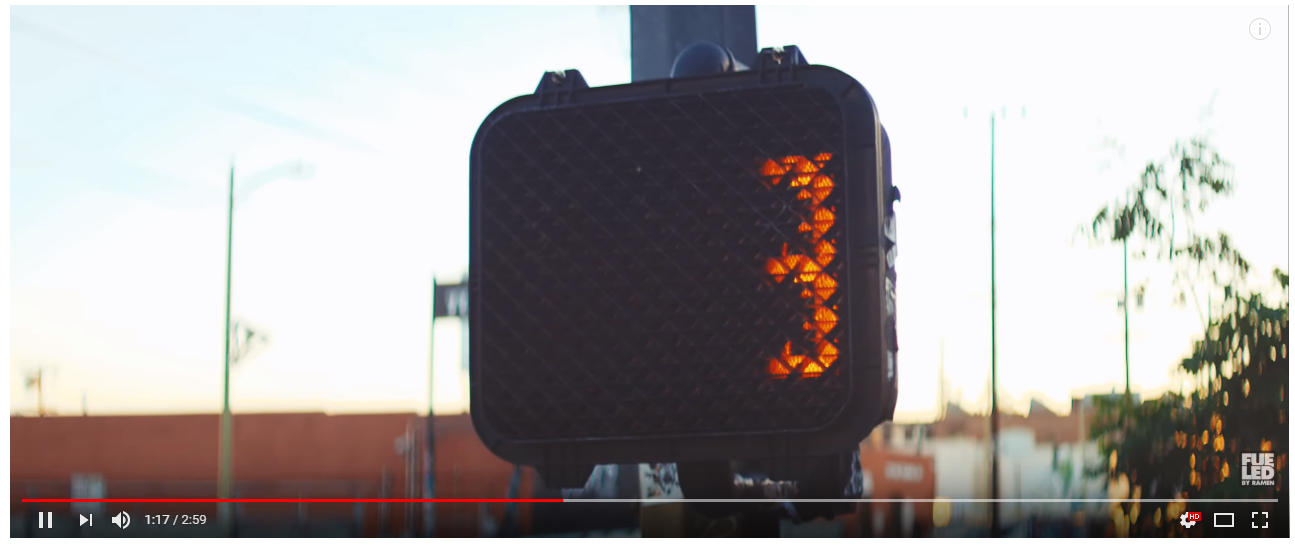
\includegraphics[width=.9\textwidth,center]{YoutubePlayer1.png}
\caption{\label{fig:YoutubePlayer1}Player der Video-Plattform \textit{Youtube} \citep{Youtube2015Panic}}
\end{figure}

In \citep{youtubeinfokarten,youtubeabspann} werden Möglichkeiten aufgezeigt, Informationen an ein Video zu annotieren. Die Informationen können Verweise auf andere Videos, Playlists und Kanäle, eine Abstimmung oder einen Link zu einer Webseite beinhalten. Einem Video können insgesamt maximal ein Abspann und bis zu fünf Infokarten mittels des integrierten Webeditors angeheftet werden. Abbildung \ref{fig:YoutubePlayer2} zeigt, wie solche Infokarten im Player dargestellt werden. Auf das Vorhandensein von Infokarten wird durch ein Infosymbol in der rechten oberen Ecke des Videos hingewiesen. Bei einem Klick auf das Symbol werden die Infokarten angezeigt. Darüber hinaus kann pro Infokarte ein beliebiger Zeitpunkt im Video festgelegt werden, zu dem ein zusätzlicher Hinweis zur Infokarte eingeblendet wird. Ein Abspann kann hingegen nur während der letzten fünf bis 20 Sekunden eines Videos angezeigt werden.

\begin{figure}[h!]
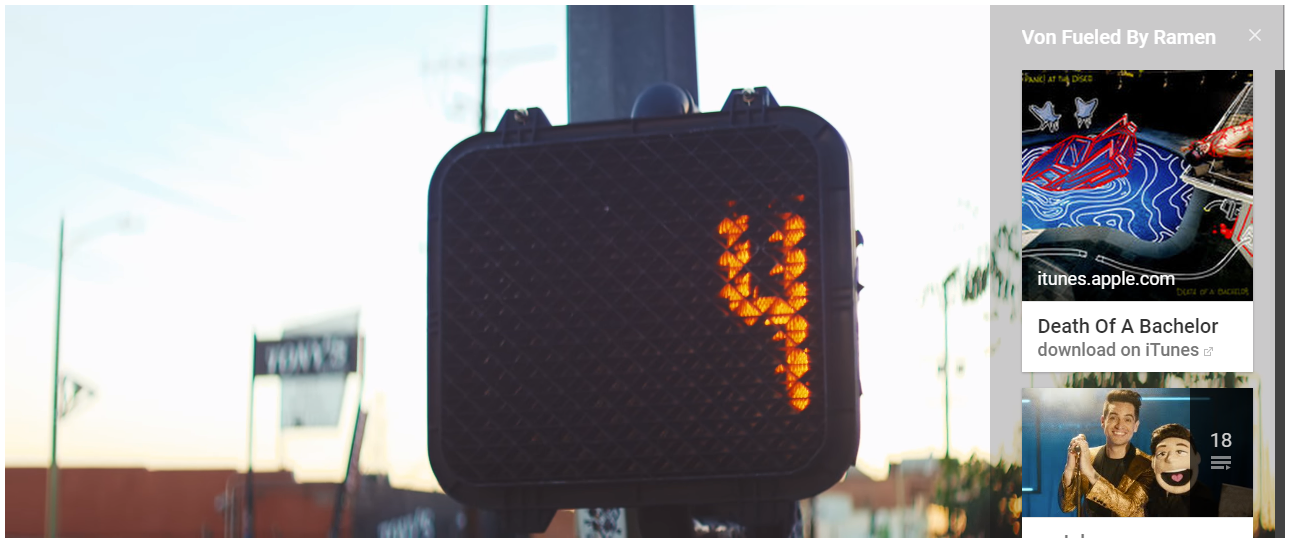
\includegraphics[width=.9\textwidth,center]{YoutubePlayer2.png}
\caption{\label{fig:YoutubePlayer2}Anzeige der Infokarten \citep{Youtube2015Panic}}
\end{figure}


%%%%%%%%%%
\subsection{Technologien für den Einsatz in Moodle}
\label{sub:TechnologienMoodle}
Im zweiten Schritt wird sich nun der Analyse bestehender Komponenten zugewendet, die als Basis für das Moodle-Plugin dienen könnten. Ziel ist es, festzustellen, ob bereits Technologien existieren, mit deren Hilfe die Idee des Hyperaudio"=Plugins umgesetzt werden kann oder ob zumindest Teile davon - unter entsprechender Beachtung der Lizenzierung - sinnvoll wiederverwendet werden können. Im Zuge dessen wird so vorgegangen, dass die einzelnen vorhanden Technologien auf diesem Gebiet mit ihren Funktionen vorgestellt werden. Dabei wird deren Relevanz für die Umsetzung des Plugins begutachtet.

%%%%%%%%%%
\subsubsection{VideoJS Player}
Bei dem \textit{VideoJS Player}\footnote{GitHub-Projekt, Apache-Lizenz 2.0: http://videojs.com/; https://github.com/videojs} handelt es sich um eine Open-Source-Bibliothek zum Abspielen von Videos und stellt damit einen HTML5-Video-Player zur Verfügung. Der \textit{VideoJS Player} ist bereits als Standard-Plugin für die Wiedergabe von Audio- und Video-Dateien in Moodle integriert. Wie der Name schon erkennen lässt, handelt es sich hierbei um eine JavaScript-Bibliothek. Der \textit{VideoJS Player} beschränkt sich in seiner Ausgangsversion ausschließlich auf das Abspielen von Audio- und Video-Dateien und bietet einen optionalen Fallback auf den Adobe FlashPlayer. Die Funktionalität des \textit{VideoJS Player} kann aber über Plugins erweitert werden. Es existieren bereits zahlreiche solcher Plugins. Hier sei vor allem das Plugin \textit{videojs-wavesurfer}\footnote{GitHub-Projekt, MIT Lizenz: https://github.com/collab-project/videojs-wavesurfer} genannt, welches das \textit{wavesurfer.js}-Framework in den \textit{VideoJS Player} integriert. Dank der Unterstützung von Plugins ist es durchaus denkbar, den Player mittels Plugin beispielsweise um Buttons zum Erstellen von Kommentaren oder persönlichen Notizen zu erweitern. Auch wäre es denkbar, mittels eines Plugins die annotierten Kommentare zu visualisieren. Grundsätzlich stellt der \textit{VideoJS Player} somit eine gute Ausgangslage für einen Hyperaudio-Player dar.

%%%%%%%%%%
\subsubsection{H5P}
Mit \textit{H5P} und dem bereits vorhanden Plugin für Moodle\footnote{GitHub-Projekt, GNU General Public License v2.0: https://github.com/h5p/h5p-moodle-plugin} ist es möglich, verschiedene Arten von interaktiven Lerninhalten zu gestalten. Dabei handelt es sich um eine Sammlung von interaktiven Komponenten, darunter \textit{Course Presentation}, \textit{Timeline} und \textit{Interactive Video}. \textit{Course Presentation} bietet die Möglichkeit, interaktive Präsentationen zu gestalten. \textit{Timeline} kann genutzt werden um Inhalte anhand eines Zeitstrahls darzustellen. \textit{Interactive Video} ermöglicht, ähnlich wie \textit{Course Presentation}, die Interaktion während des Abspielens eines Videos (siehe Abbildung \ref{fig:H5P}). Besonders erwähnenswert ist, dass sich die interaktiven Inhalte bei \textit{H5P} innerhalb der Weboberfläche erstellen lassen. Es wäre also denkbar, eine eigene interaktive Komponente zu entwickeln, welche es ermöglicht, Hyperaudio"=Dokumente als interaktiven Lerninhalt zu erstellen und abzuspielen sowie eine Kommentarfunktion zu integrieren.

\begin{figure}[h!]
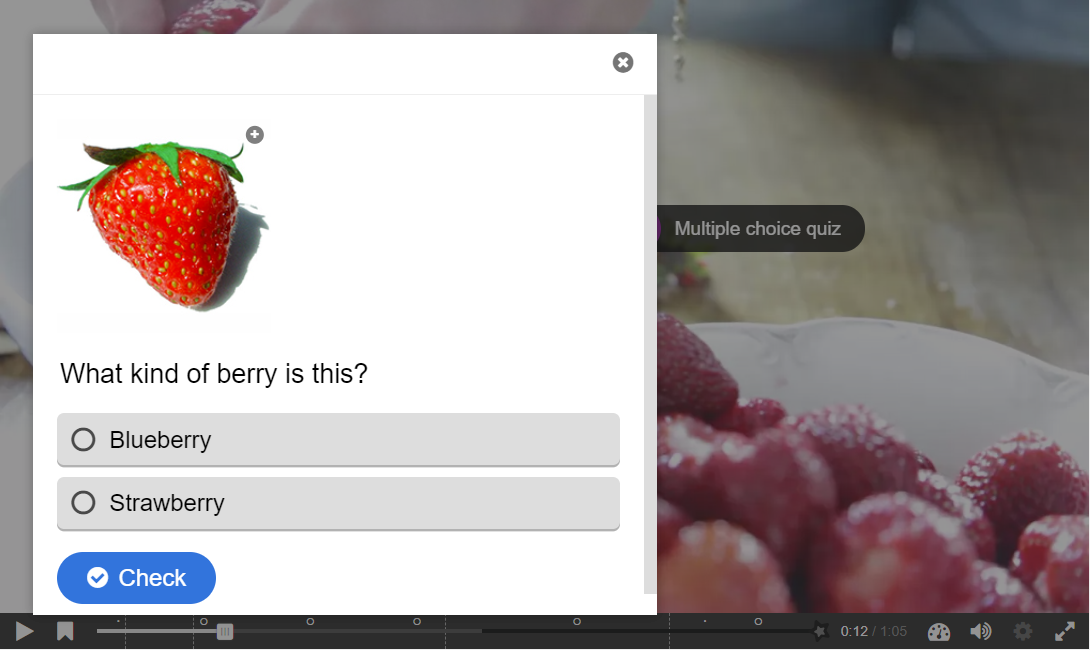
\includegraphics[width=\textwidth,center]{H5P.png}
\caption{\label{fig:H5P} Auszug aus einem \textit{Interactive Video} \citep{h5p2013video}}
\end{figure}

%%%%%%%%%%
\subsubsection{Popcorn.js}
Die Mozilla Corporation bietet mit \textit{Popcorn.js}\footnote{GitHub-Projekt, MIT Lizenz: https://github.com/mozilla/popcorn-js} eine Bibliothek an, welche neben einer standardisierten Steuerung von Medieninhalten aus verschiedenen Quellen auch die zeitabhängige Annotation von Inhalten mittels Plugins ermöglicht. Hier wäre also auch eine Entwicklung eines Plugins denkbar, mit welchem Hyperaudio"=Dokumente wie gewünscht wiedergegeben werden können. Die Wartung für die Bibliothek wurde seitens Mozilla zwar eingestellt, das Projekt steht aber weiterhin auf GitHub zur Verfügung. Obwohl das Projekt nicht mehr weiterentwickelt wird, kann es durch die vorhandenen Steuerungsmöglichkeiten und das Plugin-System ein geeignetes Grundgerüst für die Entwicklung des Moodle-Plugins darstellen.

 
%%%%%%%%%%
\subsubsection{wavesurfer.js}
\label{sec:wavesurfer.js}
Bei \textit{wavesurfer.js}\footnote{GitHub-Projekt, BSD-3-Clause: https://wavesurfer-js.org; https://github.com/katspaugh/wavesurfer.js} handelt es sich um ein JavaScript-Framework, welches es ermöglicht, die Wellenform zu der abgespielten Audio-Datei visualisieren zu lassen (siehe Abbildung \ref{fig:Wavesurfer}). Diese Basisfunktionalität wurde durch Weiterentwicklungen um nützliche Funktionen erweitert. Auf zwei dieser Weiterentwicklungen wird im Folgenden eingegangen.

\begin{figure}[h!]
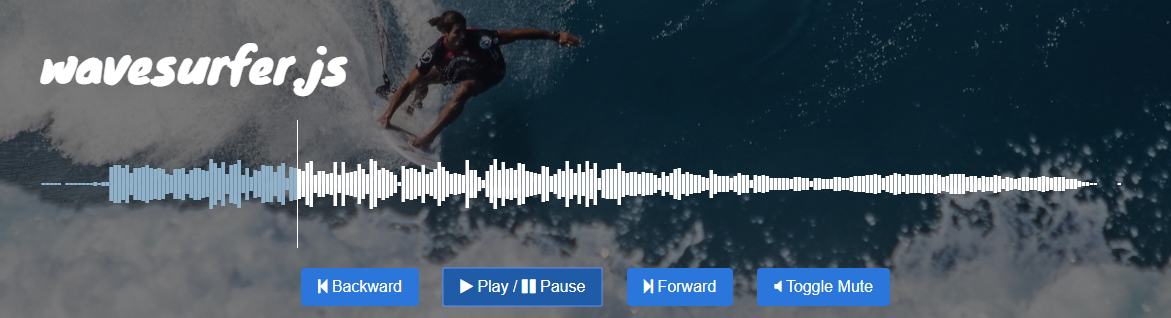
\includegraphics[width=\textwidth,center]{Wavesurfer.png}
\caption{\label{fig:Wavesurfer} Der Audio-Player auf der \textit{wavesurfer.js}-Webseite\citep{wavesurfer}}
\end{figure}


Der \textit{audio-annotator}\footnote{GitHub-Projekt, BSD-2-Clause: https://github.com/CrowdCurio/audio-annotator} stellt eine auf dem \textit{wavesurfer.js}-Framework basierende Weiterentwicklung dar, welche es mittels Weboberfläche ermöglicht, Annotationen in Form von Text an eine Audio-Datei anzuheften. Es erweitert \textit{wavesurfer.js} also um die Möglichkeit, Annotationen an eine Datei anzuheften und bietet gleichzeitig noch eine Oberfläche, um ebendiese Annotationen vorzunehmen.\\
Beim \textit{BAT - BMAT Annotation Tool}\footnote{GitHub-Projekt, GNU General Public License 3: https://wavesurfer-js.org; https://github.com/BlaiMelendezCatalan/BAT} handelt es sich um eine Entwicklung basierend auf dem Framework \textit{wavesurfer.js}. Es ermöglicht, ebenso wie \textit{audio-annotator}, dem Benutzer mittels Weboberfläche Annotationen an einer Audio-Datei vorzunehmen. Somit bietet \textit{BAT} logischerweise dieselben Vorzüge wie bereits der \textit{audio-annotator}. Im Vergleich zum \textit{audio-annotator} stellt \textit{BAT} jedoch ein weiterentwickelteres Framework dar.

Das \textit{wavesurfer.js} Framework - speziell mit seinen Weiterenticklungen - bietet einige Funktionen, die für das Abspielen von Hyperaudio"=Dokumenten nützlich sein könnten. Zusätzlich bietet es auch die Funktion,  die entsprechenden Annotationen in einer Weboberfläche an die Audio-Dateien anzuheften. Grundsätzlich lässt sich feststellen, dass \textit{wavesurfer.js} und seine Ableger im Vergleich zu den zuvor betrachteten Entwicklungen einen wesentlich unausgereifteren Eindruck hinterlassen.

%%%%%%%%%%
\subsubsection{timesheets.js}
\textit{timesheets.js}\footnote{ehemaliges GitHub-Projekt, MIT Lizenz: http://wam.inrialpes.fr/timesheets} ist ebenfalls ein JavaScript-Framemwork, welches analog zu \textit{audio-annotator} und \textit{BAT} die Annotation zusätzlicher Inhalte ermöglicht. Leider befindet sich das Framework aktuell nicht mehr in der Entwicklung. Aufgrund der Ähnlichkeit zu den {wavesurfer.js}-Ablegern und der eingestellten Entwicklung können hier zwar Ideen übernommen werden, als Basis für das zu entwickelnde Moodle-Plugin ist dieses Framework jedoch nicht geeignet.
\\\\\\
Zusammenfassend ist festzustellen, dass für die Entwicklung des Plugins für Hyperaudio"=Dokumente vor allem \textit{VideoJS Player}, \textit{H5P} und \textit{Popcorn.js} die vielversprechendsten bestehenden Entwicklungen darstellen, da diese bereits einen hohen Entwicklungsstand haben. Unter Anbetracht der benötigten Funktionen stellen aber speziell der \textit{VideoJS Player} und \textit{Popcorn.js} eine gute Basis dar, da diese mit ihrem Kernelement als Player sowie durch die integrierten Plugin-Systeme für die Entwicklung von Multimedia-Elementen ausgelegt sind. Bei \textit{H5P} müsste die Playerfunktion mit der dazugehörigen Erweiterung für Hyperaudio"=Dokumente von Grund auf entwickelt werden, um eine entsprechende interaktive Komponente für Hyperaudio"=Dokumente bereitstellen zu können. Letztlich scheint \textit{Popcorn.js} die beste Grundlage für die Entwicklung des Plugins darzustellen, da hier auch die Steuerung der Medieninhalte bereits von Grund auf ausgeprägt implementiert sind, woraus bei der Umsetzung einiger Funktionen großer Nutzen gezogen werden kann. Des Weiteren ist \textit{Popcorn.js} als JavaScript-Bibliothek mühelos als Thirdparty-Framework in Moodle integrierbar.


%%%%%%%%%%
\section{Zusammenfassung}
Im ersten Schritt der Analyse wurden Personas als mögliche Nutzer der Anwendung entwickelt. Anhand der Personas konnte die Aufteilung der Zielgruppe in Nutzende und Administrierende abgeleitet werden. Personas und Rollen wurden daraufhin zurate gezogen, um User Stories zu formulieren. Die daraus resultierenden rollenspezifischen Anforderungen wurden definiert und im Hinblick auf die Zielsetzung der Arbeit in drei Prioritätsstufen kategorisiert, welche die Basis für das Vorgehen im Implementierungsprozess bilden. Als Vorbereitung für die Implementierung dient ebenfalls die genauere Betrachtung der Möglichkeiten zur Plugin-Entwicklung in Moodle. Als Rahmenbedingung kann festgehalten werden, dass das Hyperaudio"=Plugin primär als Aktivitäten-Plugin umzusetzen ist und dass Übersichten und Favoritenfunktion innerhalb von Blöcken realisiert werden können. Bei der Betrachtung des aktuellen Stands der Technik im Allgemeinen sowie im Bezug auf die Entwicklung des Plugins wurde entschieden, dass \textit{Popcorn.js} als Grundlage für das Hyperaudio"=Plugin dienen soll, da dieses mit seinen vorhanden Steuerungs- und Annotationsmöglichkeiten ein gutes Grundgerüst darstellt und problemlos in Moodle integriert werden kann.


%%%%%%%%%%%%%%%%
\chapter{Konzept}
%% lade Kapitel aus Datei
Mit den Erkenntnissen des vorherigen Kapitels können wir uns nun der Konzeption unseres Moodle-Plugins zuwenden. Dabei werden wir zu Beginn verschiedene Nutzungsszenarien basierend auf den bereits festgelegten Anforderungen definieren. Diese sollen dann im späteren Verlauf auch zur Evaluierung der Implementierung herangezogen werden. Mit diesen Nutzungsszenarien im Hinterkopf wenden wir uns dann im nächsten Schritt der Benutzeroberfläche und deren Gestaltung zu. Abschließend haben wir ausreichend Vorarbeiten geleistet, um die Architektur des Plugins festzulegen und das Schnittstellenformat zu definieren. Diese stellen dann die letzten Schritte vor der Implementierung des Plugins dar.
\todo[inline]{komplett überarbeiten}
Der in Abbildung \ref{fig:UMLAufbau} dargestellte Zusammenhang zwischen Zusatzinhalt und Hyperaudio-Dokument kann mittels einer Schnittstellendatei umgesetzt werden. Diese wird im laufe des Kapitels genauer erörtert.

%%%%%%%%%%
\section{Zusammenhänge der Komponenten von Hyperaudio-Dokument und Annotationen}
Basierend auf der Definition eines Hyperaudio-Dokuments aus Abschnitt \ref{sec:hyperaudio} und der in Abschnitt \ref{sec:anforderungsdefinition} erarbeiteten Anforderungen werden die Zusammenhänge der medialen Komponenten weiter analysiert. Hierbei soll vor allem geklärt werden, wie die einzelnen Komponenten von Hyperaudio-Dokument und Annotationen zusammenhängen und welche Möglichkeiten dadurch gegeben beziehungsweise nicht gegeben sind.


%%%%%%%%%%
\subsection{Komponenten}
Im Mittelpunkt eines Hyperaudio-Dokuments steht eine Audio-Datei. Inhaltlich kann es sich hierbei beispielsweise um einen Vorlesungsvortrag handeln. Man könnte sich auch vorstellen, dass ein Hyperaudio-Dokument aus mehreren aneinandergereihten Audio-Dateien besteht. Dies würde an der grundsätzlichen Problemstellung jedoch nichts ändern und kann im Nachhinein jederzeit als Erweiterung umgesetzt werden. Aus diesem Grund wird in dieser Arbeit nur ein Plugin für ein Hyperaudio-Dokument bestehend aus einer Audio-Datei entwickelt.

Neben dieser zentralen Audio-Datei besteht das Hyperaudio-Dokument aus mehreren Zusatzinhalten, wobei es sich um Bilder, Graphen, Tabellen usw. handeln kann. Entscheidend ist aber, dass diese Zusatzinhalte immer nur eine rein grafische Darstellung verkörpern. Videos mit Ton sind somit beispielsweise nicht als Zusatzinhalt verwendbar, reine Animationen ohne Ton sind aber durchaus möglich.

Als besondere, nämlich externe Komponente, sind die Kommentare zu nennen. Diese gehören nicht zum eigentlichen Hyperaudio-Dokument, sollen aber mit diesem verknüpft werden. Es wird drei verschiedene Arten von Kommentaren geben, nämlich  öffentliche Kommentare, persönliche Notizen und persönliche Markierungen. Innerhalb der öffentlichen Kommentare muss noch zwischen den Original-Kommentaren und den Antworten auf diese unterschieden werden. 


%%%%%%%%%%
\subsection{Zusammenhänge}
\label{sec:komponenten_zusammenhänge}
Diese Zusammenhänge der soeben genannten Komponenten sind im UML-Diagramm in Abbildung \ref{fig:UMLAufbau} ersichtlich. Zunächst werden die Zusammenhänge zwischen der Audio-Datei und den Zusatzinhalten betrachtet. Nach dem Master-Slave-Prinzip werden Zusatzinhalte der Audio-Datei untergeordnet. Zu jedem beliebigen Zeitpunkt innerhalb der Abspieldauer der Audio-Datei kann maximal ein Zusatzinhalt gleichzeitig annotiert werden. Es sind also auch Phasen möglich, zu denen keinerlei Zusatzinhalt dargestellt wird. Das Zeitfenster für die Annotation soll mittels einer Start- und Endzeit pro Zusatzinhalt definiert werden, wobei nur die Minuten und Sekunden anzugeben sind. Bei dem Zeitfenster sollte natürlich bedacht werden, dass dieses nicht zu kurz sein sollte. Zwar soll, sobald ein Zusatzinhalt im Player des Hyperaudio-Dokuments angezeigt wird, ein entsprechender Audio Cue abgespielt werden, dennoch können bereits einige Sekunden vergehen bis der Studierende seinen Blick dem Player zuwendet.

Auch die Kommentare stehen als externe Komponente in einer gewissen Art und Weise im Zusammenhang mit der Audio-Datei. Dies ergibt sich daraus, dass Kommentare zu einem bestimmten Zeitpunkt innerhalb der Audio-Datei erfasst werden. Während Antworten auf Original-Kommentare erfasst werden können, sind Antworten auf Antworten nicht möglich.

Zwischen Kommentaren und Zusatzinhalten gibt es jedoch keinen direkten Zusammenhang. Solche Zusammenhänge ergeben sich alleine aus den Zeitpunkten der Annotationen. Zusatzinhalte können wiederum in keinem Zusammenhang mit einem anderen Zusatzinhalt stehen.


\begin{figure}[h!]
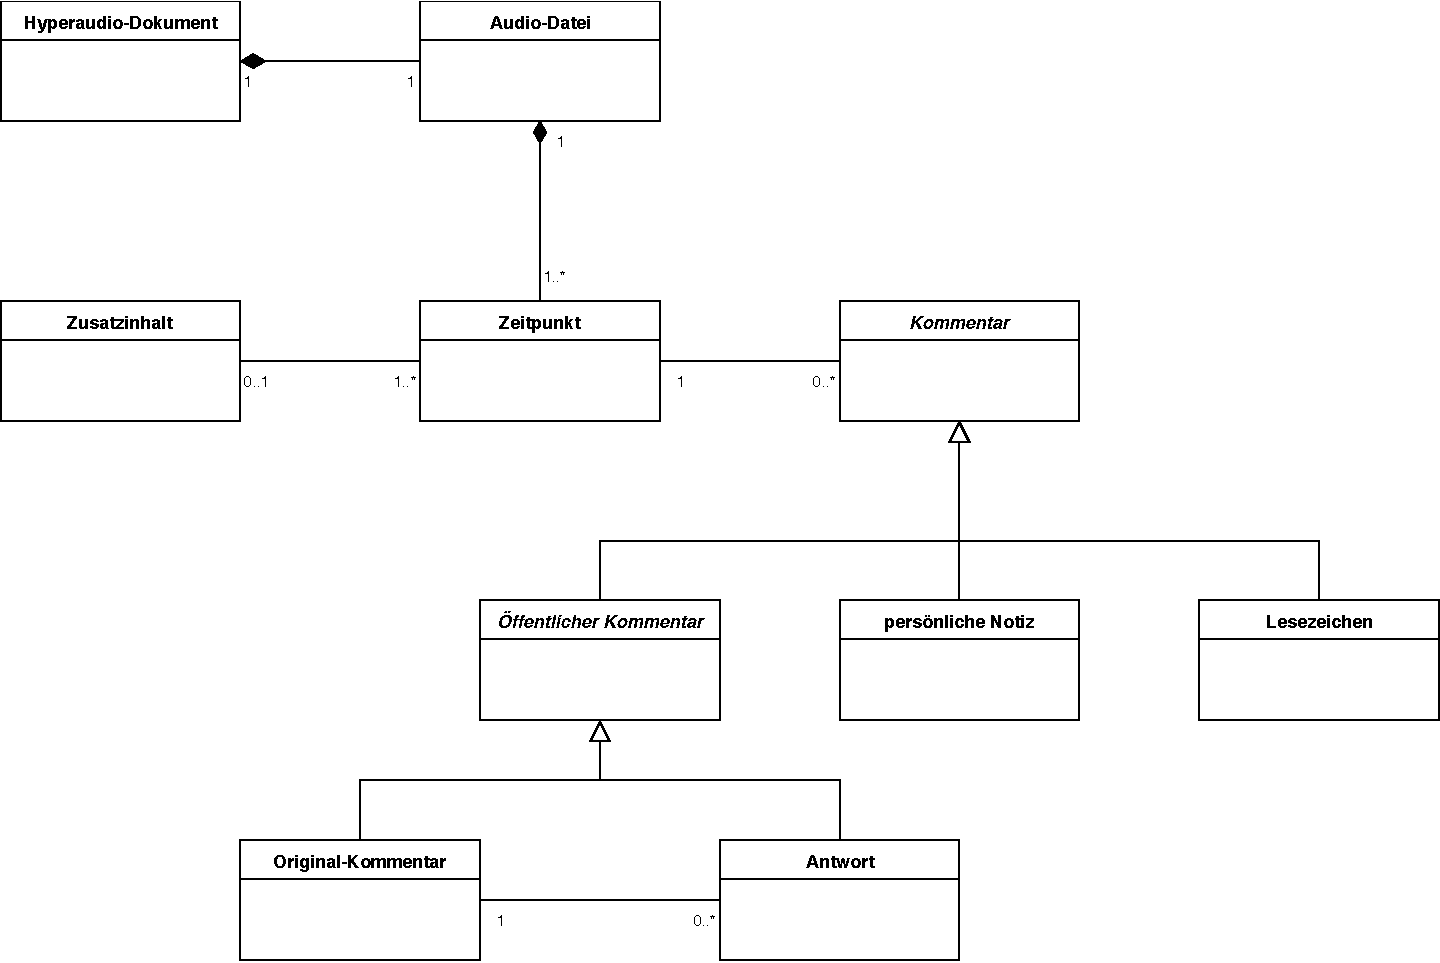
\includegraphics[width=\textwidth,center]{UMLZusammenhaenge.pdf}
\caption{\label{fig:UMLAufbau}Zusammenhänge der Komponenten}
\end{figure}


%%%%%%%%%%
\section{Definition des Schnittstellenformats für Hyperaudio-Dokumente}
\label{sec:konfigurationsdatei}
\todo[inline]{Grobe Beschreibung der Struktur und des Ablaufs...u.A. warum Schnittstellendatei notwendig ist}
\todo[inline]{Metainformationen zu Zusatzinhalten}
Wie in der Einleitung dieses Kapitels beschrieben, kann die Konfiguration zu welchem Zeitpunkt welcher Zusatzinhalt annotiert werden soll mittels einer Konfigurationsdatei durchgeführt werden. Diese Vorgehensweise wird nun umgesetzt und die Konfigurationsdatei ist entsprechend zu definieren.
Auf Grund des Einsatzes von \textit{PHP} und \textit{JavaScript} innerhalb der Moodle Plugin-Entwicklung bietet sich der Einsatz von \textit{JSON} (JavaScript Object Notation) an. \textit{JSON} wird direkt durch \textit{JavaScript} unterstützt, ist somit am besten für \textit{JavaScript} geeignet und bietet im Vergleich zu \textit{XML} erhebliche Geschwindigkeitsvorteile \citep{nurseitov2009comparison}.
%JSON is directly supported inside JavaScript [7] and is best suited for JavaScript applications; thus providing significant performance gains over XML, 
Mittels der \textit{JSON}-Datei sollen folgende Informationen der Zusatzinhalte übertragen werden:

\begin{itemize}
\item Dateiname
\item Name des Zusatzinhaltes
\item Kurseinheit
\item Betroffene Seiten innerhalb der Kurseinheit
\item Beschreibung des Zusatzinhaltes
\item Anfangszeitpunkt der Annotation
\item Endzeitpunkt der Annotation
\end{itemize}

Entscheidend ist hierbei der Dateiname, anhand des Dateinamens wird anschließend die Zuordnung der weiteren Informationen zu dem entsprechenden Eintrag in der Datenbank vorgenommen. Eine beispielhaft befüllte \textit{JSON}-Datei ist in Auflistung \ref{lst:JSON} dargestellt.

\begin{lstlisting}[basicstyle=\small,
             inputencoding={utf8}, 
             extendedchars=false,
             commentstyle=\color{black}, 
             keywordstyle=\color{black}, 
             escapeinside=``,
             linewidth=\textwidth,
             caption={Beispielhafte \textit{JSON}-Datei},
             label={lst:JSON}]             
{
  `''`additional_contents`''`: {
    `''`additional_content`''`: [
      {`''`filename`''`: `''`Bronnamberg.png`''`, `''`name`''`: `''`Sonnenuntergang Bronnamberg`''`, `''`course_unit`''`: `''`1`''`, `''`page`''`: `''`10-20`''`, `''`description`''`: `''`asdf`''`, `''`begin`''`: `''`5`''`, `''`end`''`: `''`10`''`},
      {`''`filename`''`: `''`Apple.JPG`''`, `''`name`''`: `''`Apple Rechnung`''`, `''`course_unit`''`: `''`2`''`, `''`page`''`: `''`40-50`''`, `''`description`''`: `''`asdf`''`, `''`begin`''`: `''`15`''`, `''`end`''`: `''`25`''`}
    ]
  }
}
\end{lstlisting}
\todo[inline]{JSON Beispieldaten austauschen}

%%%%%%%%%%
\section{Datenbankentwurf}
Um die dem Plugin zugrundeliegende Datenbank zu gestalten wird auf die Erkenntnisse aus Abschnitt \ref{sec:komponenten_zusammenhänge} und Abbildung \ref{fig:UMLAufbau} zurückgegriffen. Das Ergebnis ist dem ER-Diagramm in Abbildung \ref{fig:ERDiagramm} zu entnehmen.

Jede der Tabellen verfügt über den Primärschlüssel \textit{id}. Darüber hinaus wird zu jedem Eintrag gespeichert, wann dieser erstellt (\textit{timecreated}) und zuletzt bearbeitet (\textit{timemodified}) wurde. Für das Abspeichern von Dateien stellt Moodle die Tabelle \textit{files} bereit \citep{moodle2018file}. Dort kann die Datei abgelegt und an anderer Stelle darauf referenziert werden.

Im Mittelpunkt des Hyperaudio-Plugins steht die Tabelle \textit{hyperaudio}. Diese repräsentiert das Hyperaudio-Dokument und die Audio-Datei aus Abbildung \ref{fig:UMLAufbau}. Zunächst wird die ID des Moodle-Kurses (\textit{course}) abgelegt, dem das Hyperaudio-Dokument zugeordnet ist. Während die Audio-Datei selbst in der bereits erwähnten Tabelle \textit{files} zu finden ist, wird in der Tabelle \textit{hyperaudio} deren Dateiname (\textit{audiofile}) festgehalten. Zum Hyperaudio-Dokument können außerdem Name und Ersteller in den Spalten \textit{name} und \textit{author} hinterlegt werden. Eine optionale Beschreibung kann entsprechend dem de-facto-Standard der Moodle-Plugin-Entwicklung über \textit{introformat} und \textit{intro} hinzugefügt werden \citep{moodle2016activity}.

Bei der Tabelle \textit{hyperaudio\_config} handelt es sich um eine Tabelle, in welcher die in Abschnitt \ref{sec:konfigurationsdatei} beschriebene Konfigurationsdatei gespeichert wird (\textit{file} enthält den Dateinamen als Referenz auf die \textit{files}-Tabelle). Daneben wird nur noch der Fremdschlüssel \textit{hyperaudio\_id} auf die Tabelle \textit{hyperaudio} als Zuordnung zum Hyperaudio-Dokument benötigt.

\todo[inline]{name in hyperaudio\_config entfernen}

Zur Ablage der annotierten Zusatzinhalte dient die Tabelle \textit{additional\_content}. Auch hier steht der Name der Datei in der Spalte \textit{file} als Referenz auf die \textit{files}-Tabelle. Ebenso dient der Fremdschlüssel \textit{hyperaudio\_id} zur Verknüpfung des Zusatzinhalts mit dem Hyperaudio-Dokument. Des Weiteren werden folgende Metainformationen zum Zusatzinhalt abgespeichert:

\begin{itemize}

\item Name des Zusatzinhalts (\textit{name})
\item optional: Beschreibung (\textit{description})
\item optional: Kurseinheit (\textit{course\_unit})
\item optional: Seitenangabe (\textit{page})
\item Startzeitpunkt der Annotation innerhalb des Hyperaudio-Dokuments (\textit{begin})
\item Endzeitpunkt der Annotation innerhalb des Hyperaudio-Dokuments (\textit{end})

\end{itemize}

Die Tabelle \textit{hyperaudio\_comments} dient der Speicherung der vier in Abbildung \ref{fig:UMLAufbau} modellierten Kommentararten. Der Zusammenhang zum Hyperaudio-Dokument wird analog per Fremdschlüssel \textit{hyperaudio\_id} hergestellt. Neben dem textuellen Kommentar (\textit{commenttext}), werden auch der Verfasser in Form der \textit{userid}, die Art des Kommentars (\textit{comment\_type}) und der Annotationszeitpunkt (\textit{timeannotated}) gespeichert. Für den Fall, dass es sich um einen Antwortkommentar handelt, wird in der Spalte \textit{comment\_id} die Referenz auf den Original-Kommentar festgehalten.

\begin{figure}[h!]
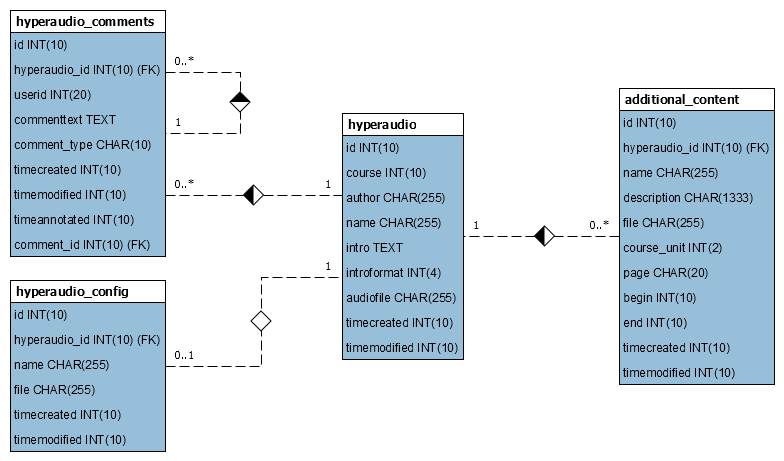
\includegraphics[width=\textwidth,center]{ERDiagramm.png}
\caption{\label{fig:ERDiagramm}ER-Diagramm der Datenbank des Moodle-Plugins}
\end{figure}


%%%%%%%%%%
\section{Gestaltung der Benutzeroberfläche}
Damit den Lehrenden und Studierenden die im vorherigen Abschnitt beschriebenen Nutzungsszenarien möglichst leicht fallen, wenden wir uns nun der Gestaltung der Benutzeroberfläche zu. \glqq Das Design der Benutzeroberfläche stellt einen zentralen Aspekt für die Gebrauchstauglichkeit eines Softwareprodukts dar\grqq{} \citep[S. 1]{oppermann2002user}. Einen dementsprechend hohen Stellenwert wollen wir der Benutzeroberfläche unseres Moodle-Plugins zuschreiben. Bei der Gestaltung der Benutzeroberfäche gehen wir wie bereits bei der Analyse in Kapitel \ref{cha:analyse} vor und teilen die Benutzeroberfläche in Teilbereiche auf. Im ersten Schritt betrachten wir zunächst die Seite eines Hyperaudio-Dokuments innerhalb eines Kurses. Danach widmen wir uns der Administrationsseite eines Hyperaudio-Dokuments innerhalb eines Kurses. Im letzten Schritt wenden wir uns den verschiedenen Integrationsmöglichkeiten innerhalb der allgemeinen Moodle-Oberfläche zu.

Generell erfolgen alle Entscheidungen bezüglich der Oberfläche auf Basis von Skizzen. Diese wurden mittels des Programms \textit{Balsamiq Mockups 3.5.15}\footnote{https://balsamiq.com/} erstellt. Anhand der Skizzen können Vor- und Nachteile der verschiedenen Designansätze schnell erkannt und auf Grund dessen sachliche Entscheidungen getroffen werden. 
%Durch das Arbeiten mit Skizzen erkennt man schneller welche Vor- und Nachteile die verschiedenen Designansätze bieten und kann auf Grund dessen dann sachliche Entscheidungen treffen.


%%%%%%%%%%
%\subsection{Seite eines Hyperaudio-Dokuments}
Die Seite eines Hyperaudio-Dokuments lässt sich grob, wie bereits in Abbildung \ref{fig:MockupBereiche} dargestellt, in die Bereiche Player, Galerie und Kommentarsektion aufteilen. Wir werden nun zunächst für jeden dieser Bereiche verschiedene Designs diskutieren und uns dann für eines entscheiden. Danach erfolgt die Entscheidung über die Anordnung dieser Bereiche auf der Seite eines Hyperaudio-Dokuments.


%%%%%%%%%%
\subsubsection{Player}
Beim Player für Hyperaudio-Dokumente müssen, neben den üblichen Mediensteuerungselementen, gleich mehrere zusätzliche Elemente visualisiert werden. Zum einen müssen zu den entsprechenden Zeitpunkten die annotierten Zusatzinhalte dargestellt werden. Auf der anderen Seiten sollen auch die annotierten öffentlichen Kommentare, persönlichen Notizen und Markierungen veranschaulicht werden. Dem Wunsch, direkt über den Player öffentliche Kommentare, persönlichen Notizen und Markierungen erstellen und in letzterem Fall sogar löschen zu können, muss auch Sorge getragen werden.

Der Player für Hyperaudio-Dokumente wird, wie in Abbildung \ref{fig:MockupPlayerVersion1} zusehen ist, als Videoplayer umgesetzt. Somit werden die Zusatzinhalte an Stelle eines Videos dargestellt. Die persönlichen Notizen und Markierungen werden innerhalb der Abspielleiste mittels unterschiedlich gefärbter Kreisen illustriert. In diesem Fall sollen die roten Kreise Markierungen und der blaue Kreis eine persönliche Notiz widerspiegeln. Unterhalb der Mediensteuerung ist ein Bereich zu finden, in dem die Kommentare grafisch sichtbar gemacht werden sollen. Hierfür wird jedes Hyperaudio-Dokument in die gleiche fixe Anzahl an Zeitfenstern aufgeteilt. Diese Zeitfenster werden durch senkrecht orientierte Balken dargestellt, deren Höhe für die Anzahl der zu diesem Zeitfenster erfassten Kommentare stehen soll. Unter dem Bereich für die Kommentare befindet sich eine Eingabemaske, mit welcher öffentliche Kommentare und persönliche Notizen erfasst werden können. Das Erstellen und Löschen von Markierungen soll mittels Rechtsklick auf die entsprechende Stelle innerhalb der Abspielleiste in einem dazugehörigen Kontextmenü umgesetzt werden. Dies ist in Abbildung \ref{fig:MockupPlayerVersion1} mittels der beiden Mauszeiger, den Pfeilen und den entsprechenden Buttons symbolisiert.

\todo[inline]{Unterscheidung nicht nur durch Farbe (Barrierefreiheit)}

%\begin{figure}[h!]
%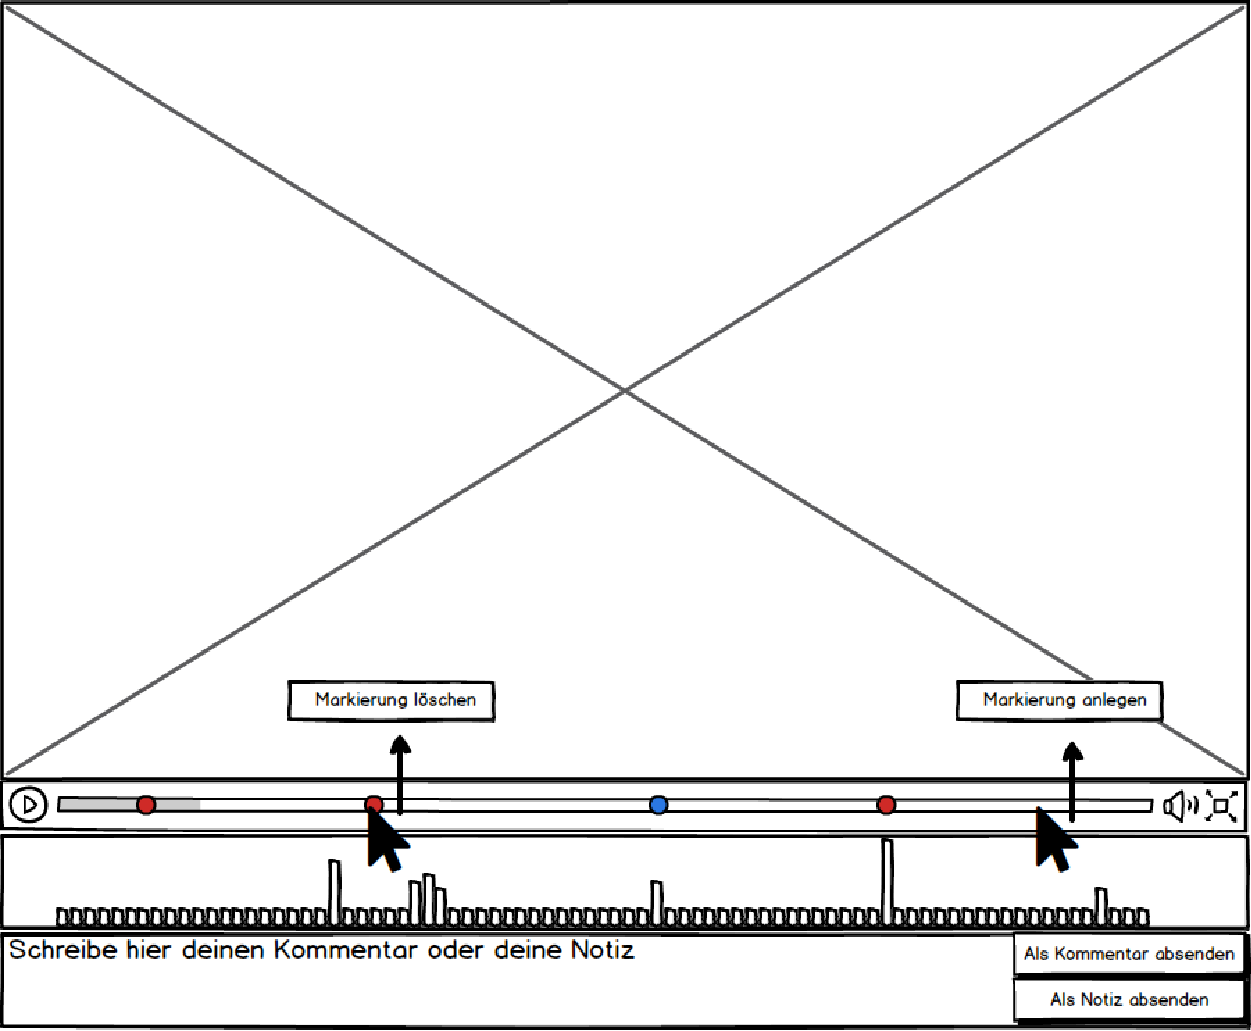
\includegraphics[width=0.8\textwidth,center]{MockupPlayerVersion1.pdf}
%\caption{\label{fig:MockupPlayerVersion1} Erster Entwurf des Players}
%\end{figure}

In einer zweiten Variante des Players wird die Visualisierung der persönlichen Notizen von der Abspielleiste in den Bereich der Kommentare verschoben. Wie in Abbildung \ref{fig:MockupPlayerVersion2} ersichtlich,  wird der Balken für den Zeitraum, in dem die persönlichen Notiz liegt, zu einem gewissen Teil blau eingefärbt. Dadurch wird nebenbei das Handling der Punkte in der Abspielleiste vereinheitlicht, da es hier nur noch die Markierungen mit Interaktionsmöglichkeit gibt.

\begin{figure}[h!]
\begin{subfigure}[c]{\textwidth}
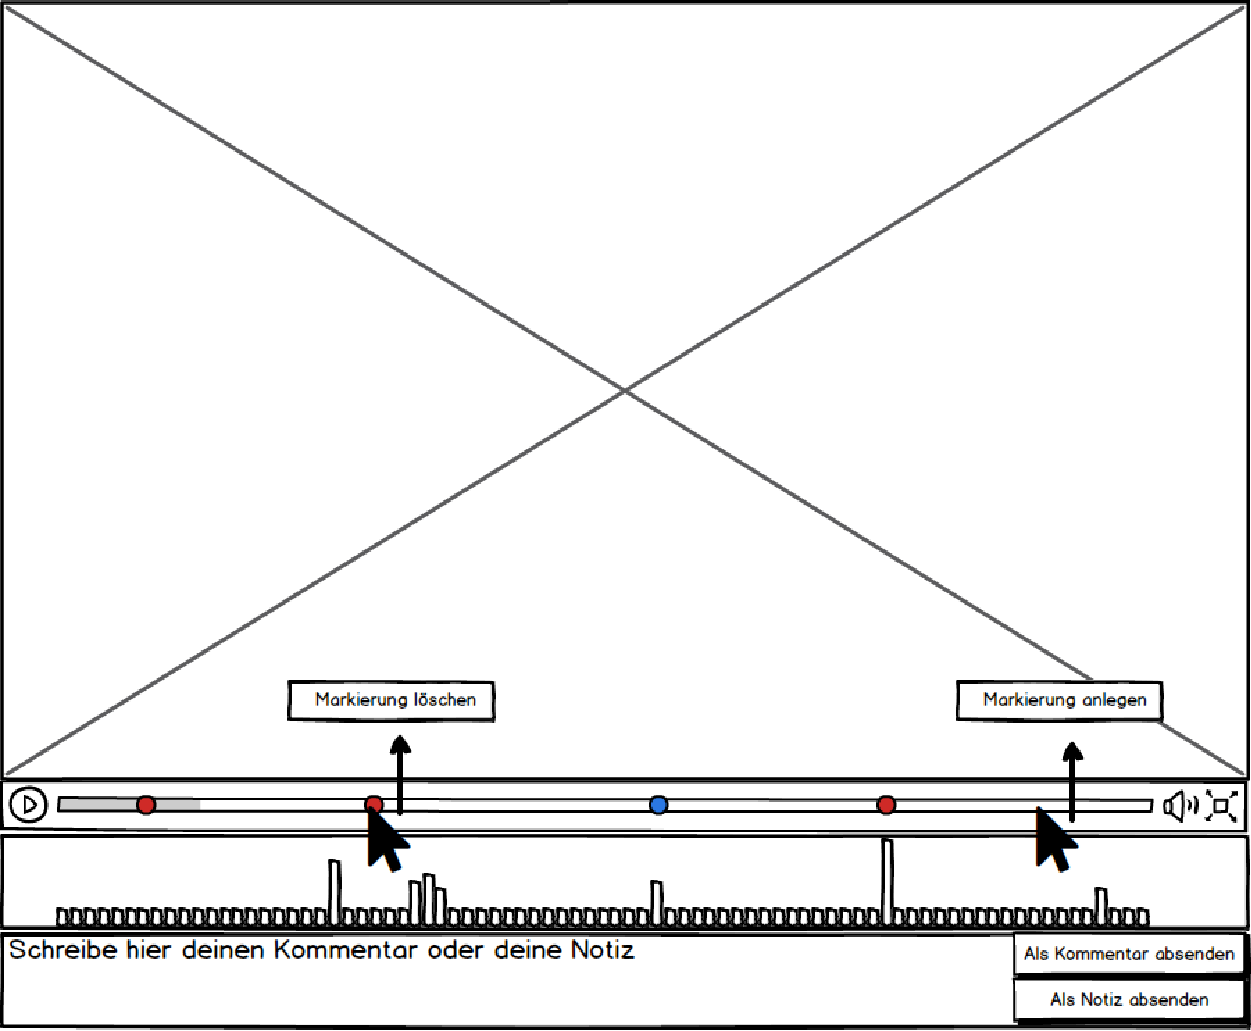
\includegraphics[width=0.8\textwidth,center]{MockupPlayerVersion1.pdf}
\subcaption{Erste Version}
\label{fig:MockupPlayerVersion1}
\end{subfigure}
\par\bigskip
\begin{subfigure}[c]{\textwidth}
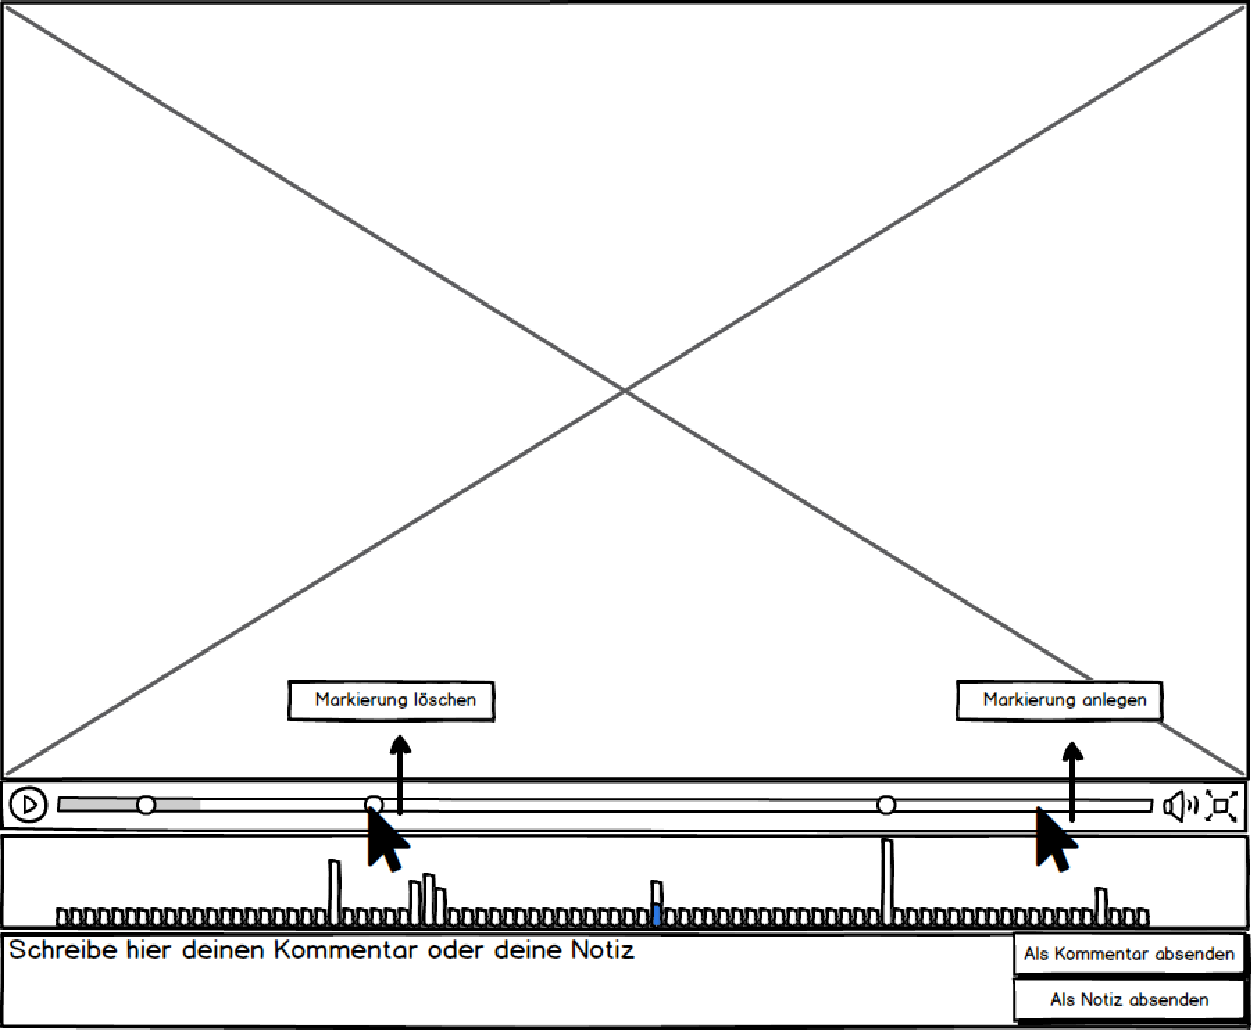
\includegraphics[width=0.8\textwidth,center]{MockupPlayerVersion2.pdf}
\subcaption{Finale Version}
\label{fig:MockupPlayerVersion2}
\end{subfigure}
\caption{Benutzeroberfläche - Player}
\label{fig:MockupPlayerVersion}
\end{figure}

%\begin{figure}[h!]
%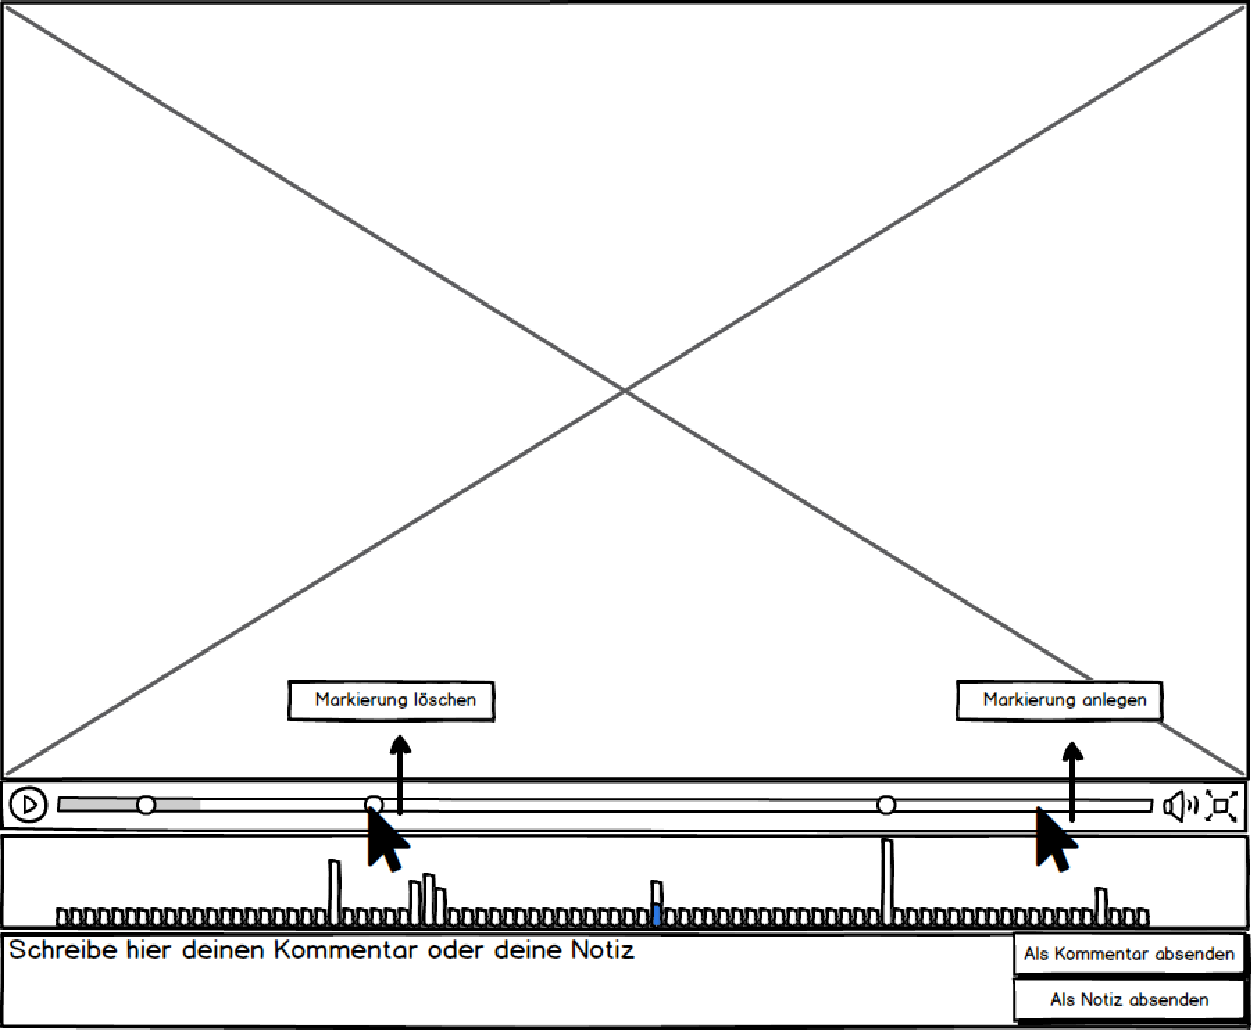
\includegraphics[width=.8\textwidth,center]{MockupPlayerVersion2.pdf}
%\caption{\label{fig:MockupPlayerVersion22}Zweiter Entwurf des Players}
%\end{figure}


%%%%%%%%%%
\subsubsection{Galerie}
Die Galerie soll dazu dienen, einen Überblick über die vorhanden Zusatzinhalte zu bieten. Die Zusatzinhalte stellen alle einen grafischen Inhalt dar. Dementsprechend kann jeder Zusatzinhalt durch ein kleines Vorschaubild repräsentiert werden. 
Eine weitere Grundfunktionalität einer Galerie ist die vergrößerte Anzeige der in der Vorschau dargestellten Inhalte, die auch in unserer Galerie zur Verfügung stehen soll. Beim Erstellen des Designs muss zusätzlich auch die Anforderung der Rückkopplung zum Player bedacht werden (siehe Abschnitt \ref{sub:AnforderungenOberflaeche}). 
%Neben der Grundfunktionalität einer Galerie, dass der ausgewählte Zusatzinhalt vergrößert angezeigt werden können soll, muss beim Erstellen des Designs auch die Anforderung der Rückkopplung zum Player bedacht werden (siehe Abschnitt \ref{sub:AnforderungenOberflaeche}). 

Die einfachste Umsetzung der Galerie ist eine Darstellung der Zusatzinhalte in einem einfachen Grid  mit Scrollbalken, wie es in Abbildung \ref{fig:MockupGalerieGrid} zu sehen ist. Zusätzlich wird das Grid um zwei Buttons für eine vergrößerte Ansicht des Zusatzinhalts sowie für die Rückkopplung zum Player ergänzt. Um eine dieser beiden Aktionen auszuführen, müsste also der gewünschte Zusatzinhalt markiert und der entsprechende Button betätigt werden.

%\begin{figure}[h!]
%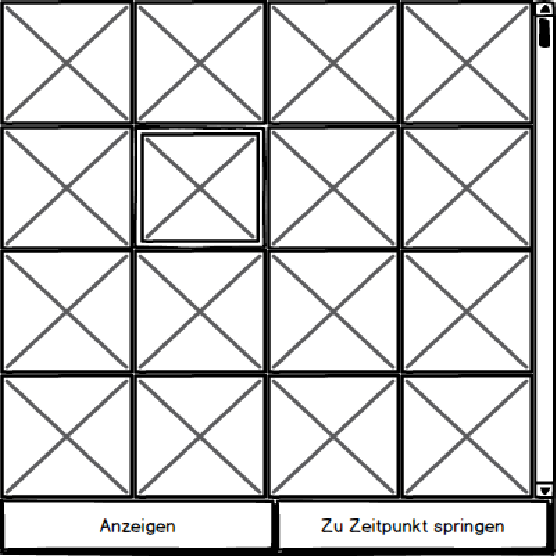
\includegraphics[width=.5\textwidth,center]{MockupGalerieGrid.pdf}
%\caption{\label{fig:MockupGalerieGrid}Garlerie als einfaches Grid}
%\end{figure}

Diese Variante hat den Vorteil, dass besonders viele Zusatzinhalte gleichzeitig angezeigt werden können. Auf der anderen Seite erhalten wir aber keinerlei Informationen zu den Zusatzinhalten. In der zweiten Variante, bei dem das Grid um einen Bereich für Details ergänzt wurde, kann man zumindest die Details des ausgewählten Zusatzinhaltes einsehen. Diese in Abbildung \ref{fig:MockupGalerieGridErweitert} erkennbaren Details sind natürlich von den vorhandenen Metadaten abhängig. Nachteil ist in diesem Fall aber, dass, durch den Bereich für die Details, bei gleicher Größe der Galerie weniger Zusatzinhalte zur selben Zeit dargestellt werden können. Das führt dazu, dass die Verwendung des Scrollbalkens häufiger notwendig wird.

%\begin{figure}[h!]
%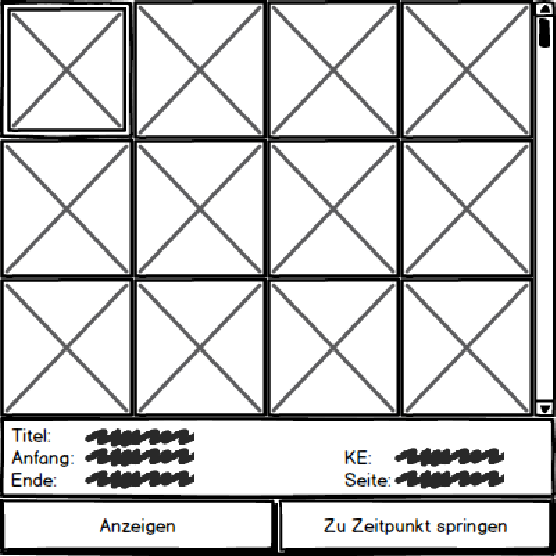
\includegraphics[width=.5\textwidth,center]{MockupGalerieGridErweitert.pdf}
%\caption{\label{fig:MockupGalerieGridErweitert}Galerie als Grid mit Bereich für Details}
%\end{figure}

Bei einer Darstellung der Zusatzinhalte als Kacheln, wie in Abbildung \ref{fig:MockupGalerieKacheln} zu sehen, können gleichzeitig für alle vorhandenen Zusatzinhalte die Details angezeigt werden. Durch diese Art der Darstellung passen jedoch noch weniger Zusatzinhalte auf die gleiche Fläche.

%\begin{figure}[h!]
%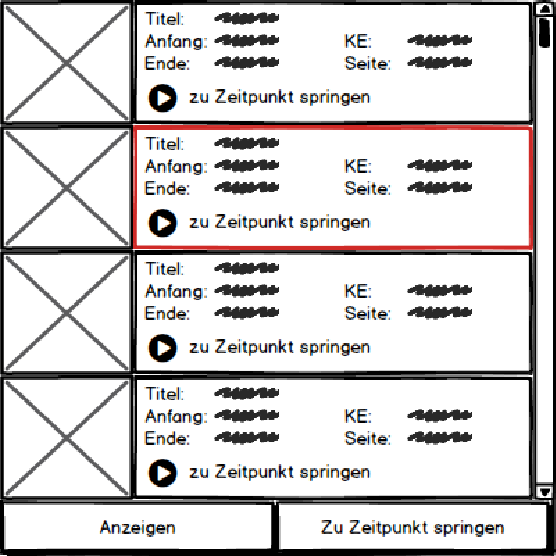
\includegraphics[width=.5\textwidth,center]{MockupGalerieKacheln.pdf}
%\caption{\label{fig:MockupGalerieKacheln}Galerie mit Darstellung in Kachelform}
%\end{figure}

Eine besonders schicke Art der Darstellung wäre die des Cover Flows, bekannt aus verschiedenen Musikplayern. In Abbildung \ref{fig:MockupGalerieCoverFlow} ist zu erkennen, dass auch hier ausschließlich Details des aktuell ausgewählten Zusatzinhaltes sichtbar sind. Des Weiteren hat diese Darstellungsweise den großen Nachteil, dass auch nicht auf einen Blick alle verfügbaren Zusatzinhalte ersichtlich sind. Dies erschwert das Durchsuchen der Zusatzinhalte ungemein. Somit ist diese Art der Darstellung zwar schön anzusehen, aber nicht sonderlich gebrauchstauglich im Zusammenhang dieser Arbeit.

%\begin{figure}[h!]
%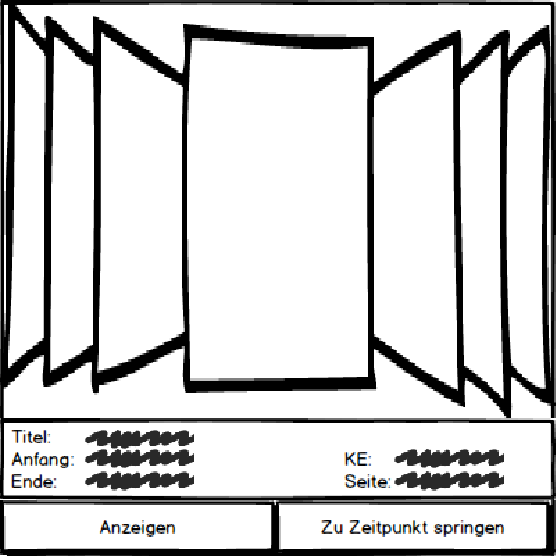
\includegraphics[width=.5\textwidth,center]{MockupGalerieCoverFlow.pdf}
%\caption{\label{fig:MockupGalerieCoverFlow}Galerie als Cover Flow}
%\end{figure}

Letztlich stellt sich die optimierte Variante der Kachel Darstellung aus Abbildung \ref{fig:MockupGalerieFinal} als beste Lösung heraus. Die Optimierung besteht daraus, dass die beiden Buttons obsolet gemacht werden. Dies kann zum einen erreicht werden, indem die vergrößerte Darstellung durch einen Klick auf die Abbildung des Zusatzinhaltes ausgelöst wird. Zum anderen bietet der Bereich der Details noch ausreichend Platz, um hier die Funktion zur Rückkopplung an den Player einzufügen. Durch diese Verbesserungen wird nicht nur mehr Platz geschaffen, sondern auch die Benutzerfreundlichkeit erhöht, indem der Vorgang zum Anzeigen der vergrößerten Ansicht beziehungsweise des Springens an den entsprechenden Zeitpunkt jeweils um einen Klick reduziert wurde.

\begin{figure}[h!]
\begin{subfigure}[c]{0.5\textwidth}
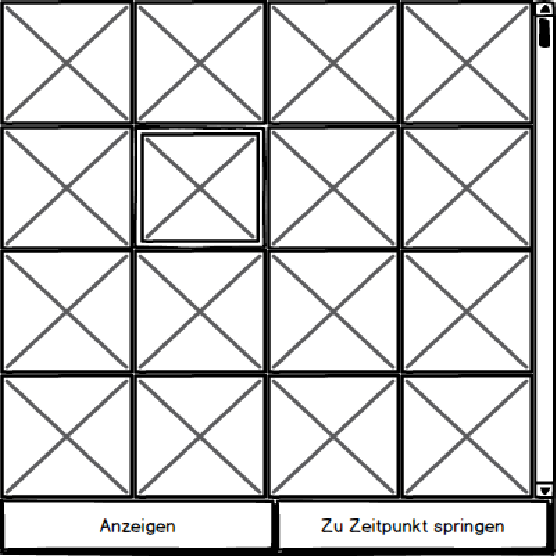
\includegraphics[width=0.8\textwidth,center]{MockupGalerieGrid.pdf}
\subcaption{Galerie als einfaches Grid}
\label{fig:MockupGalerieGrid}
\end{subfigure}%
\begin{subfigure}[c]{0.5\textwidth}
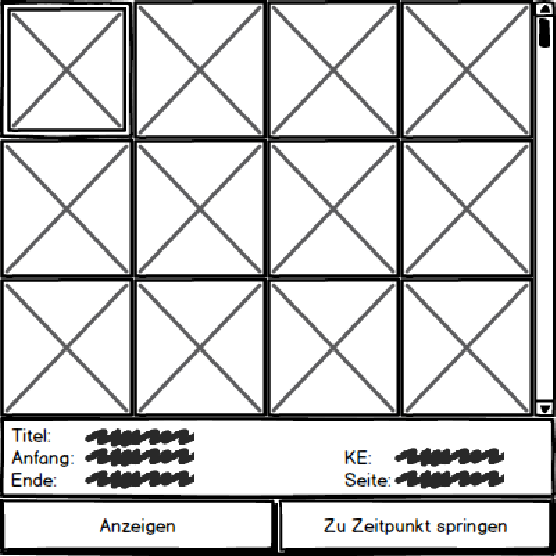
\includegraphics[width=0.8\textwidth,center]{MockupGalerieGridErweitert.pdf}
\subcaption{Galerie als Grid mit Bereich für Details}
\label{fig:MockupGalerieGridErweitert}
\end{subfigure}
\par\bigskip
\begin{subfigure}[c]{0.5\textwidth}
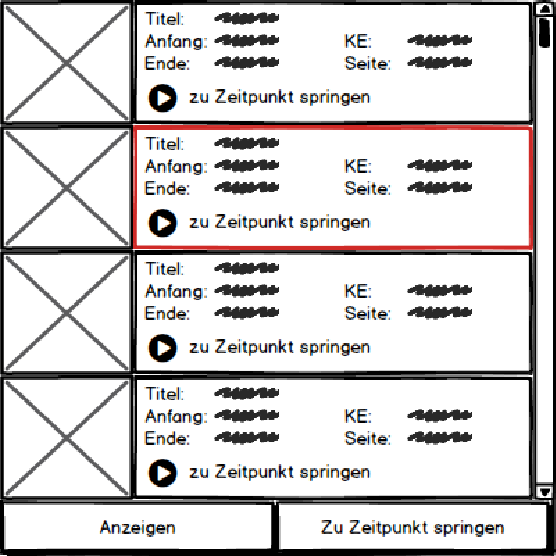
\includegraphics[width=0.8\textwidth,center]{MockupGalerieKacheln.pdf}
\subcaption{Galerie mit Darstellung in Kachelform}
\label{fig:MockupGalerieKacheln}
\end{subfigure}%
\begin{subfigure}[c]{0.5\textwidth}
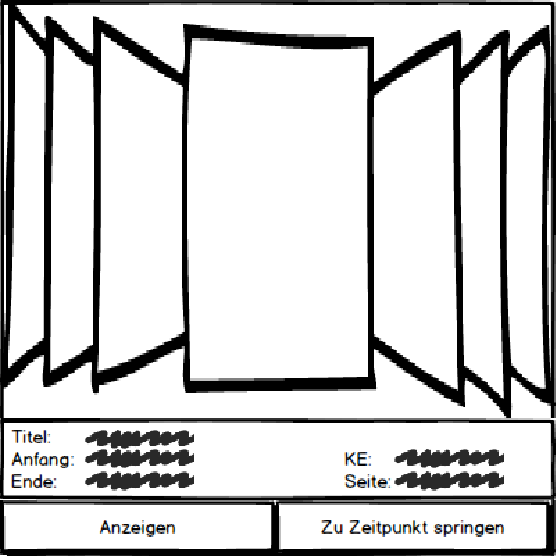
\includegraphics[width=0.8\textwidth,center]{MockupGalerieCoverFlow.pdf}
\subcaption{Galerie als Cover Flow}
\label{fig:MockupGalerieCoverFlow}
\end{subfigure}
\par\bigskip
\begin{subfigure}[c]{\textwidth}
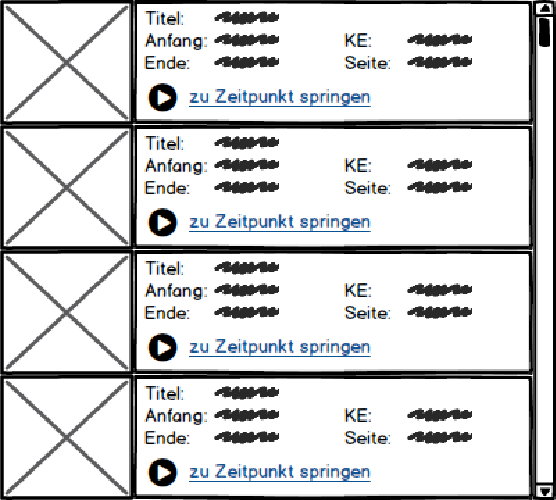
\includegraphics[width=0.4\textwidth,center]{MockupGalerieFinal.pdf}
\subcaption{Finale Version der Galerie}
\label{fig:MockupGalerieFinal}
\end{subfigure}
\caption{Benutzeroberfläche - Galerie}
\label{fig:MockupGalerie}
\end{figure}


%\begin{figure}[h!]
%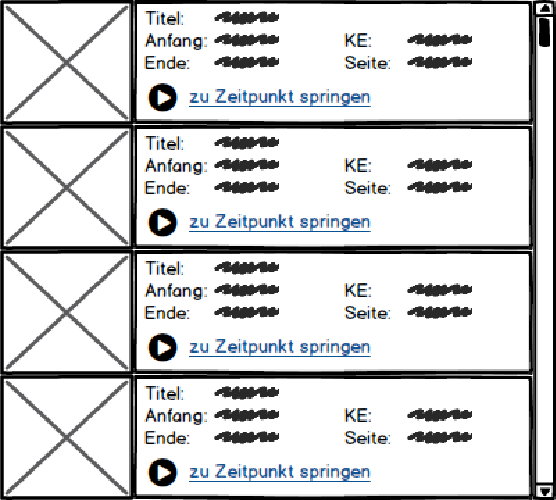
\includegraphics[width=.5\textwidth,center]{MockupGalerieFinal.pdf}
%\caption{\label{fig:MockupGalerieFinal}Finale Version der Galerie}
%\end{figure}

%%%%%%%%%%
\subsubsection{Kommentarsektion}
Die Kommentarsektion ist für die Anzeige der öffentlichen Kommentare sowie der persönlichen Notizen zuständig. Zusätzlich muss eine Suchmaske auf Basis der Anforderungen aus Abschnitt \ref{sub:AnforderungenKommentarsektion} in die Oberfläche integriert werden.

Abbildung \ref{fig:MockupKommentarsektionVersion1} zeigt eine erste Version der Kommentarsektion. Neben der Suchmaske im Kopfbereich befinden sich zwei Checkboxen. Diese ermöglichen es dem Betrachter nach öffentlichen Kommentaren und persönlichen Notizen zu filtern. Im benachbarten Dropdown-Menü kann die Grundlage der Sortierung bestimmt werden. Die Sortierung kann nach Erstellungsdatum beziehungsweise nach Zeitpunkt der Annotation innerhalb des Hyperaudio-Dokuments erfolgen. Unterhalb dieser Funktionen befindet sich die Anzeige der Kommentare und Notizen. Sowohl bei Kommentaren als auch bei Notizen wird neben dem Erstellungsdatum auch der Annotationszeitpunkt festgehalten. Dieser wird als Link umgesetzt, sodass bei einem Klick die Rückkopplung an den Player erfolgen kann. Bei Kommentaren gibt es nach Betätigung der \textit{Antworten}-Schaltfläche noch eine zusätzliche Eingabemaske zum Verfassen von Antworten. Persönliche Notizen werden durch ein Schloss-Symbol hinter dem Erstellungsdatum visualisiert. Zusätzlich befinden sich noch jeweils zwei Buttons zum Bearbeiten und Löschen auf der rechten Seite einer Notiz.

%\begin{figure}[h!]
%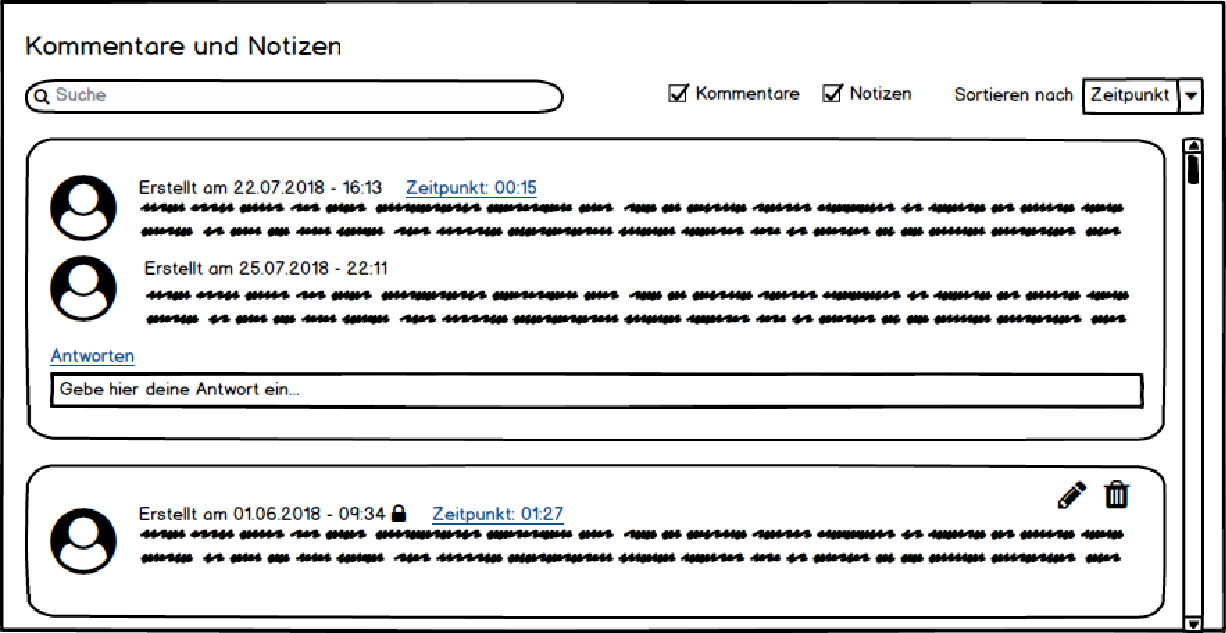
\includegraphics[width=\textwidth,center]{MockupKommentarsektionVersion1.pdf}
%\caption{\label{fig:MockupKommentarsektionVersion1}Erste Version der Kommentarsektion}
%\end{figure}

Im nochmals verbesserten Design der Kommentarsektion, welches in Abbildung \ref{fig:MockupKommentarsektionFinal} abgebildet ist, werden die Antworten auf Kommentare eingerückt dargestellt. Diese Darstellung führt zu einer besseren Übersichtlichkeit und ist auch aus anderen modernen Anwendungen bekannt.

\begin{figure}[h!]
\begin{subfigure}[c]{\textwidth}
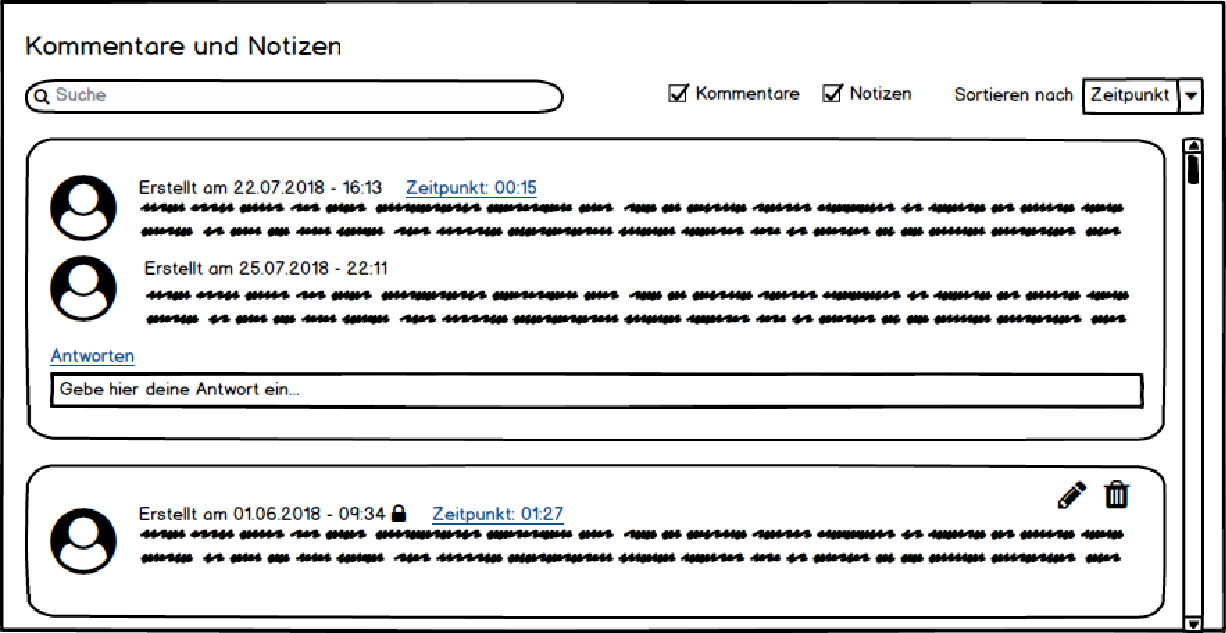
\includegraphics[width=\textwidth,center]{MockupKommentarsektionVersion1.pdf}
\subcaption{Erste Version}
\label{fig:MockupKommentarsektionVersion1}
\end{subfigure}
\par\bigskip
\begin{subfigure}[c]{\textwidth}
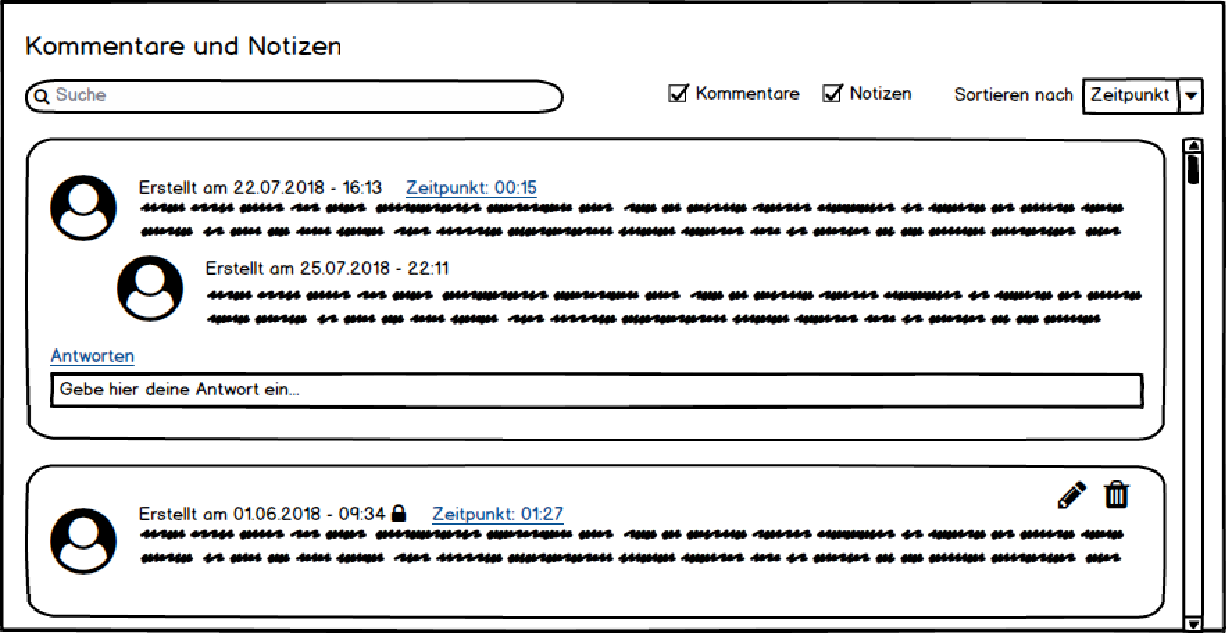
\includegraphics[width=\textwidth,center]{MockupKommentarsektionFinal.pdf}
\subcaption{Finale Version}
\label{fig:MockupKommentarsektionFinal}
\end{subfigure}
\caption{Benutzeroberfläche - Kommentarsektion}
\label{fig:MockupKommentarsektion}
\end{figure}

%\begin{figure}[h!]
%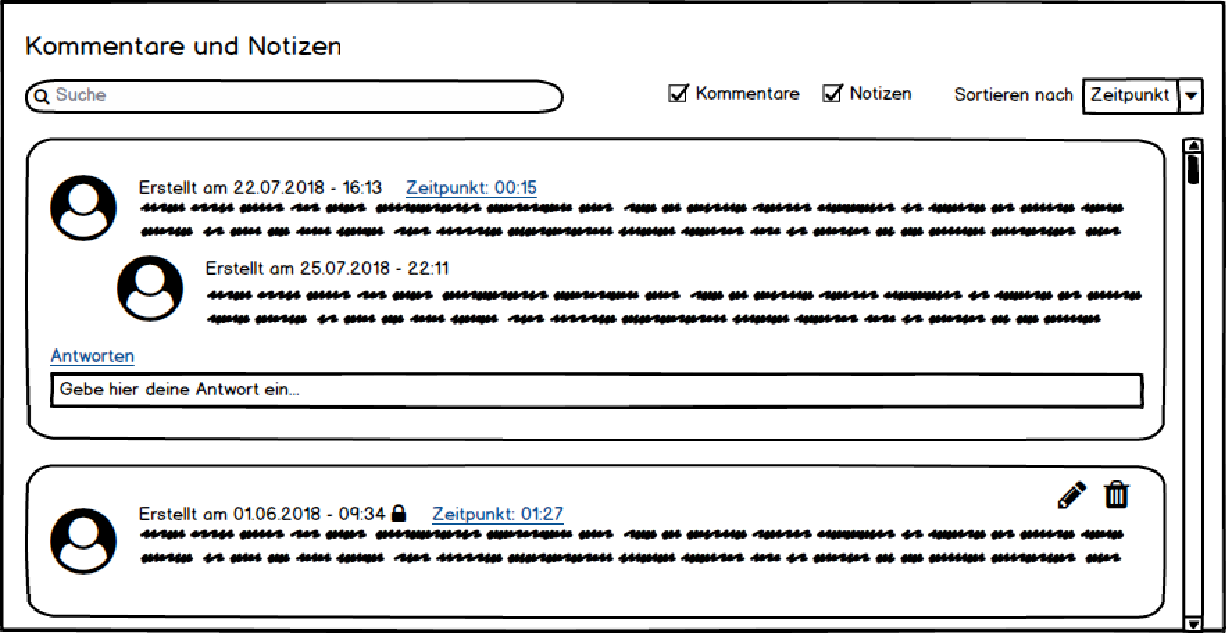
\includegraphics[width=\textwidth,center]{MockupKommentarsektionFinal.pdf}
%\caption{\label{fig:MockupKommentarsektionFinal}Finale Version der Kommentarsektion}
%\end{figure}


%%%%%%%%%%
\subsubsection{Zusammenführen der Elemente}
Im ersten Schritt führen wir die jeweils favorisierten Elemente in ein Layout zusammen. Dabei orientieren wir uns zunächst an unserer grobe Skizze aus Kapitel \ref{cha:analyse}. Wie nun in Abbildung \ref{fig:MockupSeiteLayoutVersion1} zu erkennen ist, ist die Kommentarsektion so in die Breite gezogen, dass das Lesen der Inhalte unangenehm werden kann. Aus diesem Grund wird in der finalen Version (siehe Abbildung \ref{fig:MockupSeiteLayoutFinal}) die Breite der Kommentarsektion auf die Breite des Players beschränkt. Dies hat zeitgleich zur Folge, dass der nun vorhandene freie Platz für die Galerie verwendet werden kann. Spätestens hiermit wird der Nachteil der gewählten Darstellungsweise der Galerie egalisiert, da nun ausreichend viele Zusatzinhalte ohne die Verwendung des Scrollbalkens eingesehen werden können.

%\begin{figure}[h!]
%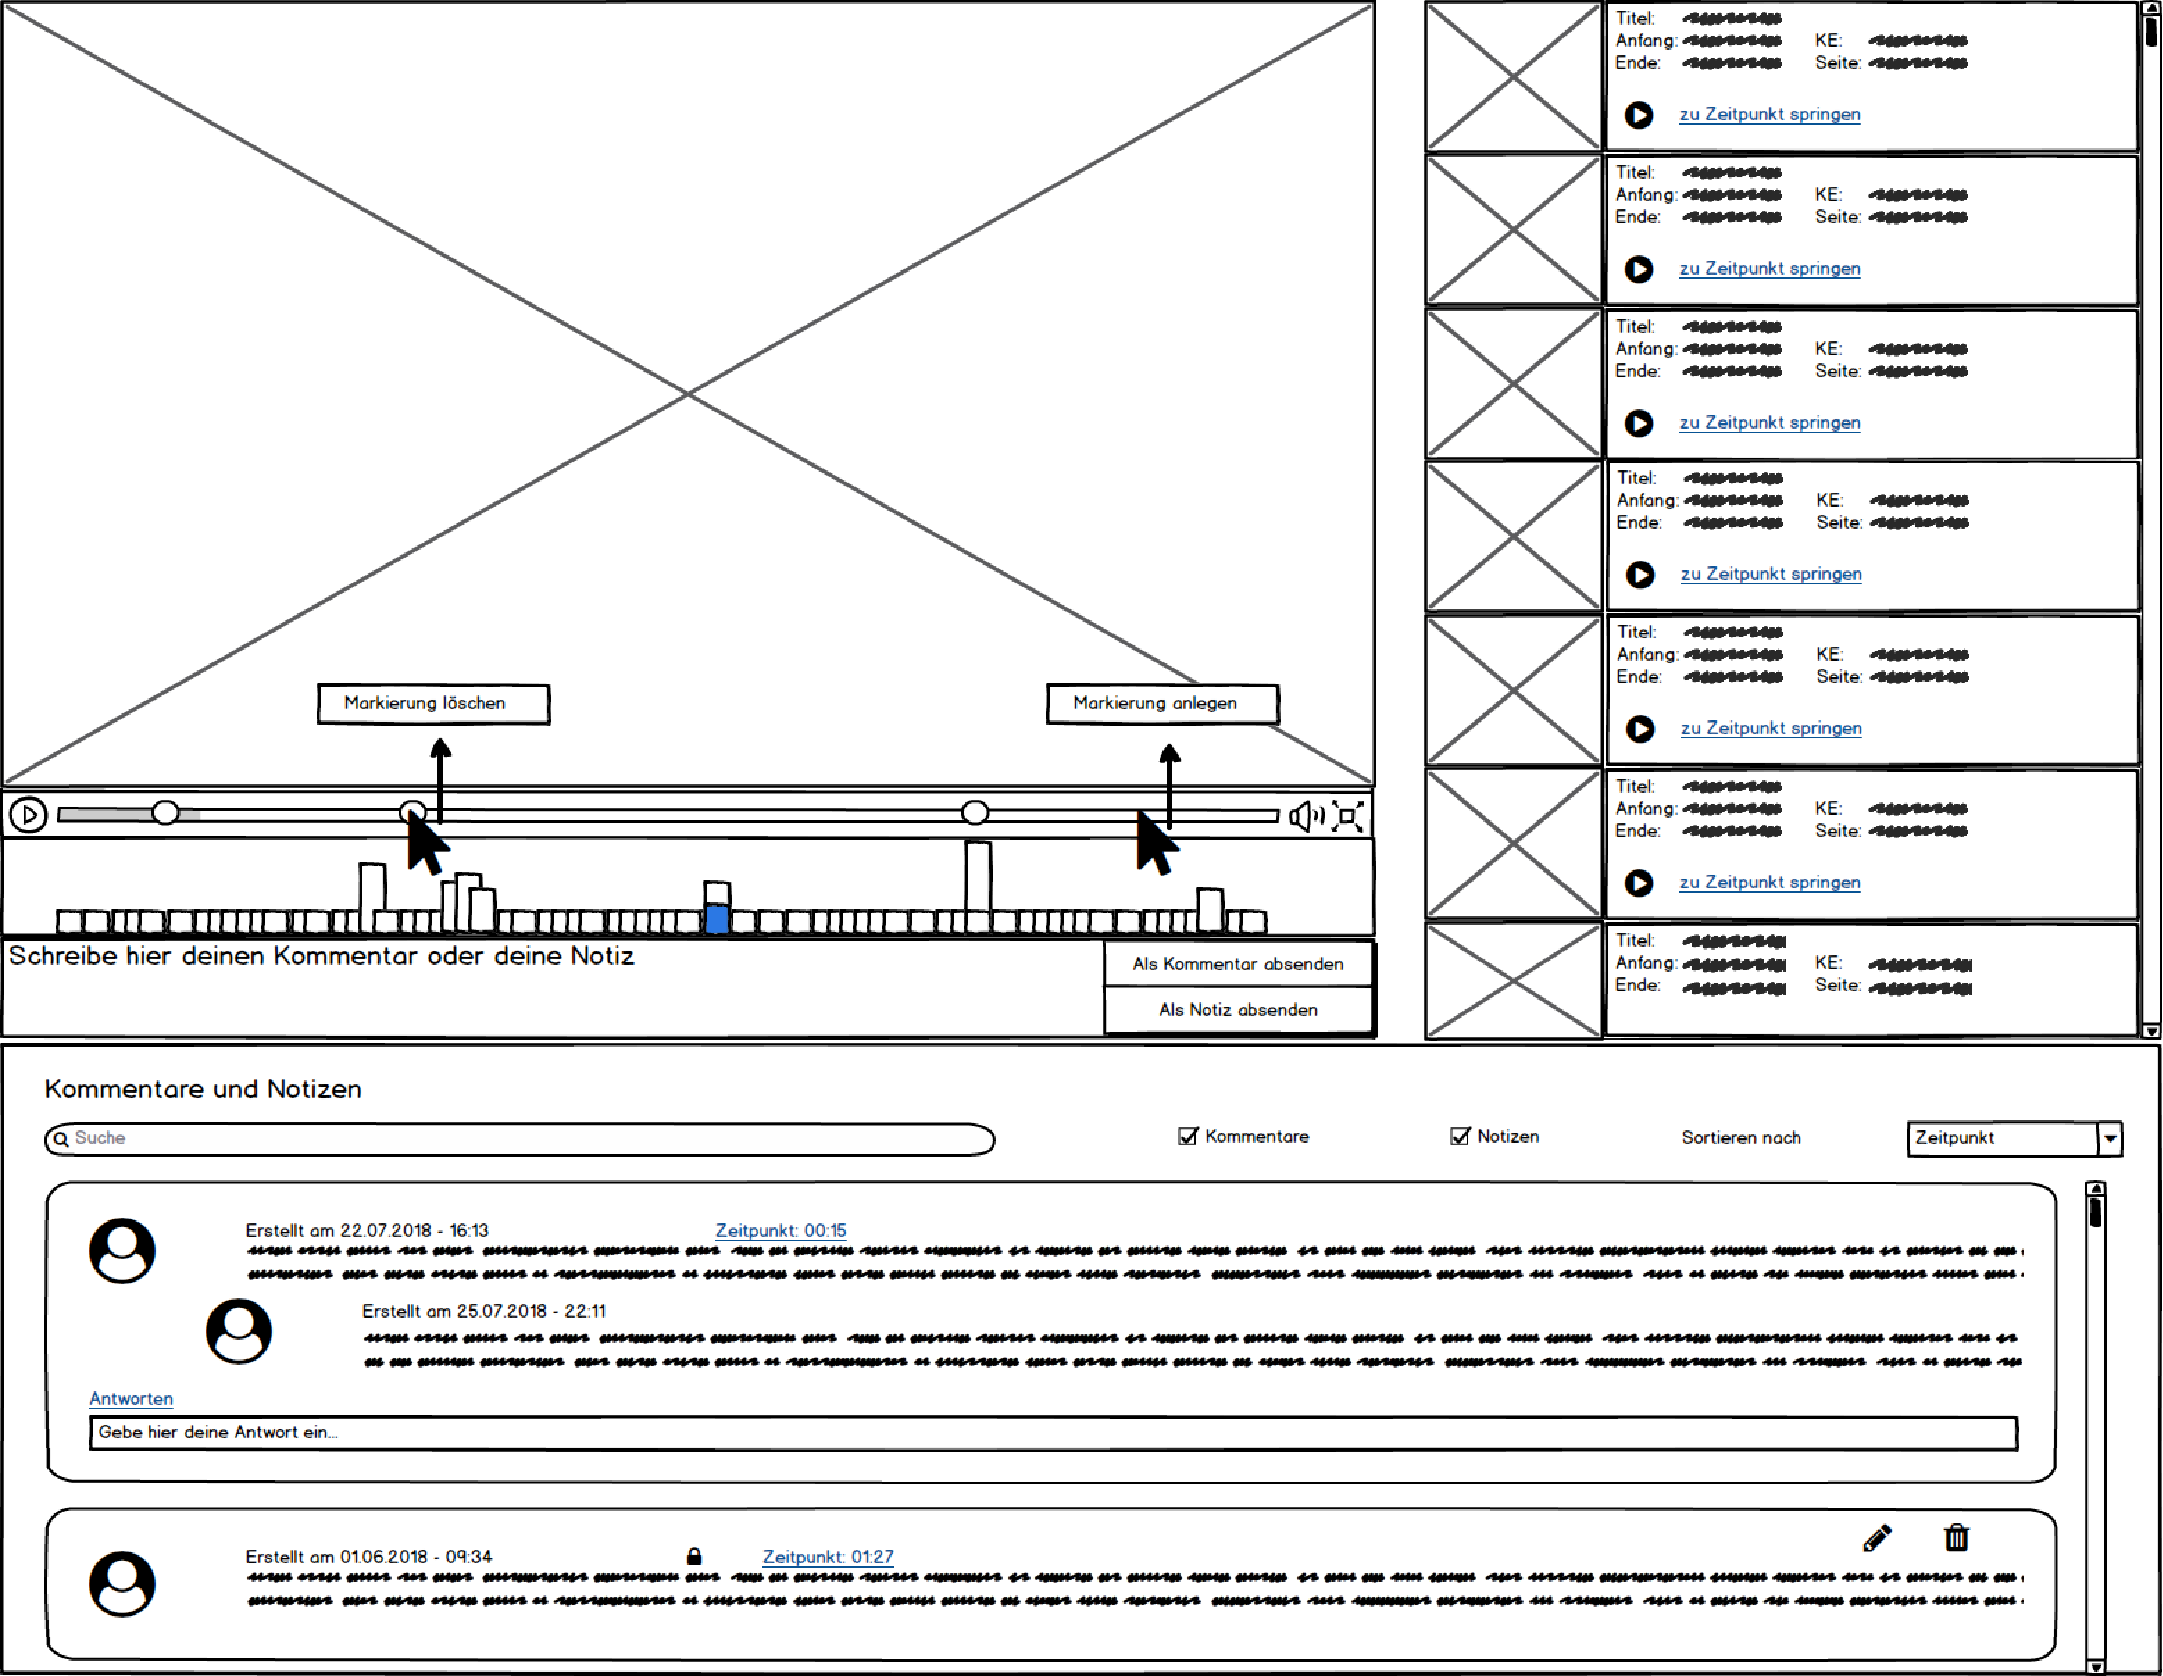
\includegraphics[width=\textwidth,center]{MockupSeiteLayoutVersion1.pdf}
%\caption{\label{fig:MockupSeiteLayoutVersion1}Erstes Layout der Seite für Hyperaudio-Dokumente}
%\end{figure}

%\begin{figure}[h!]
%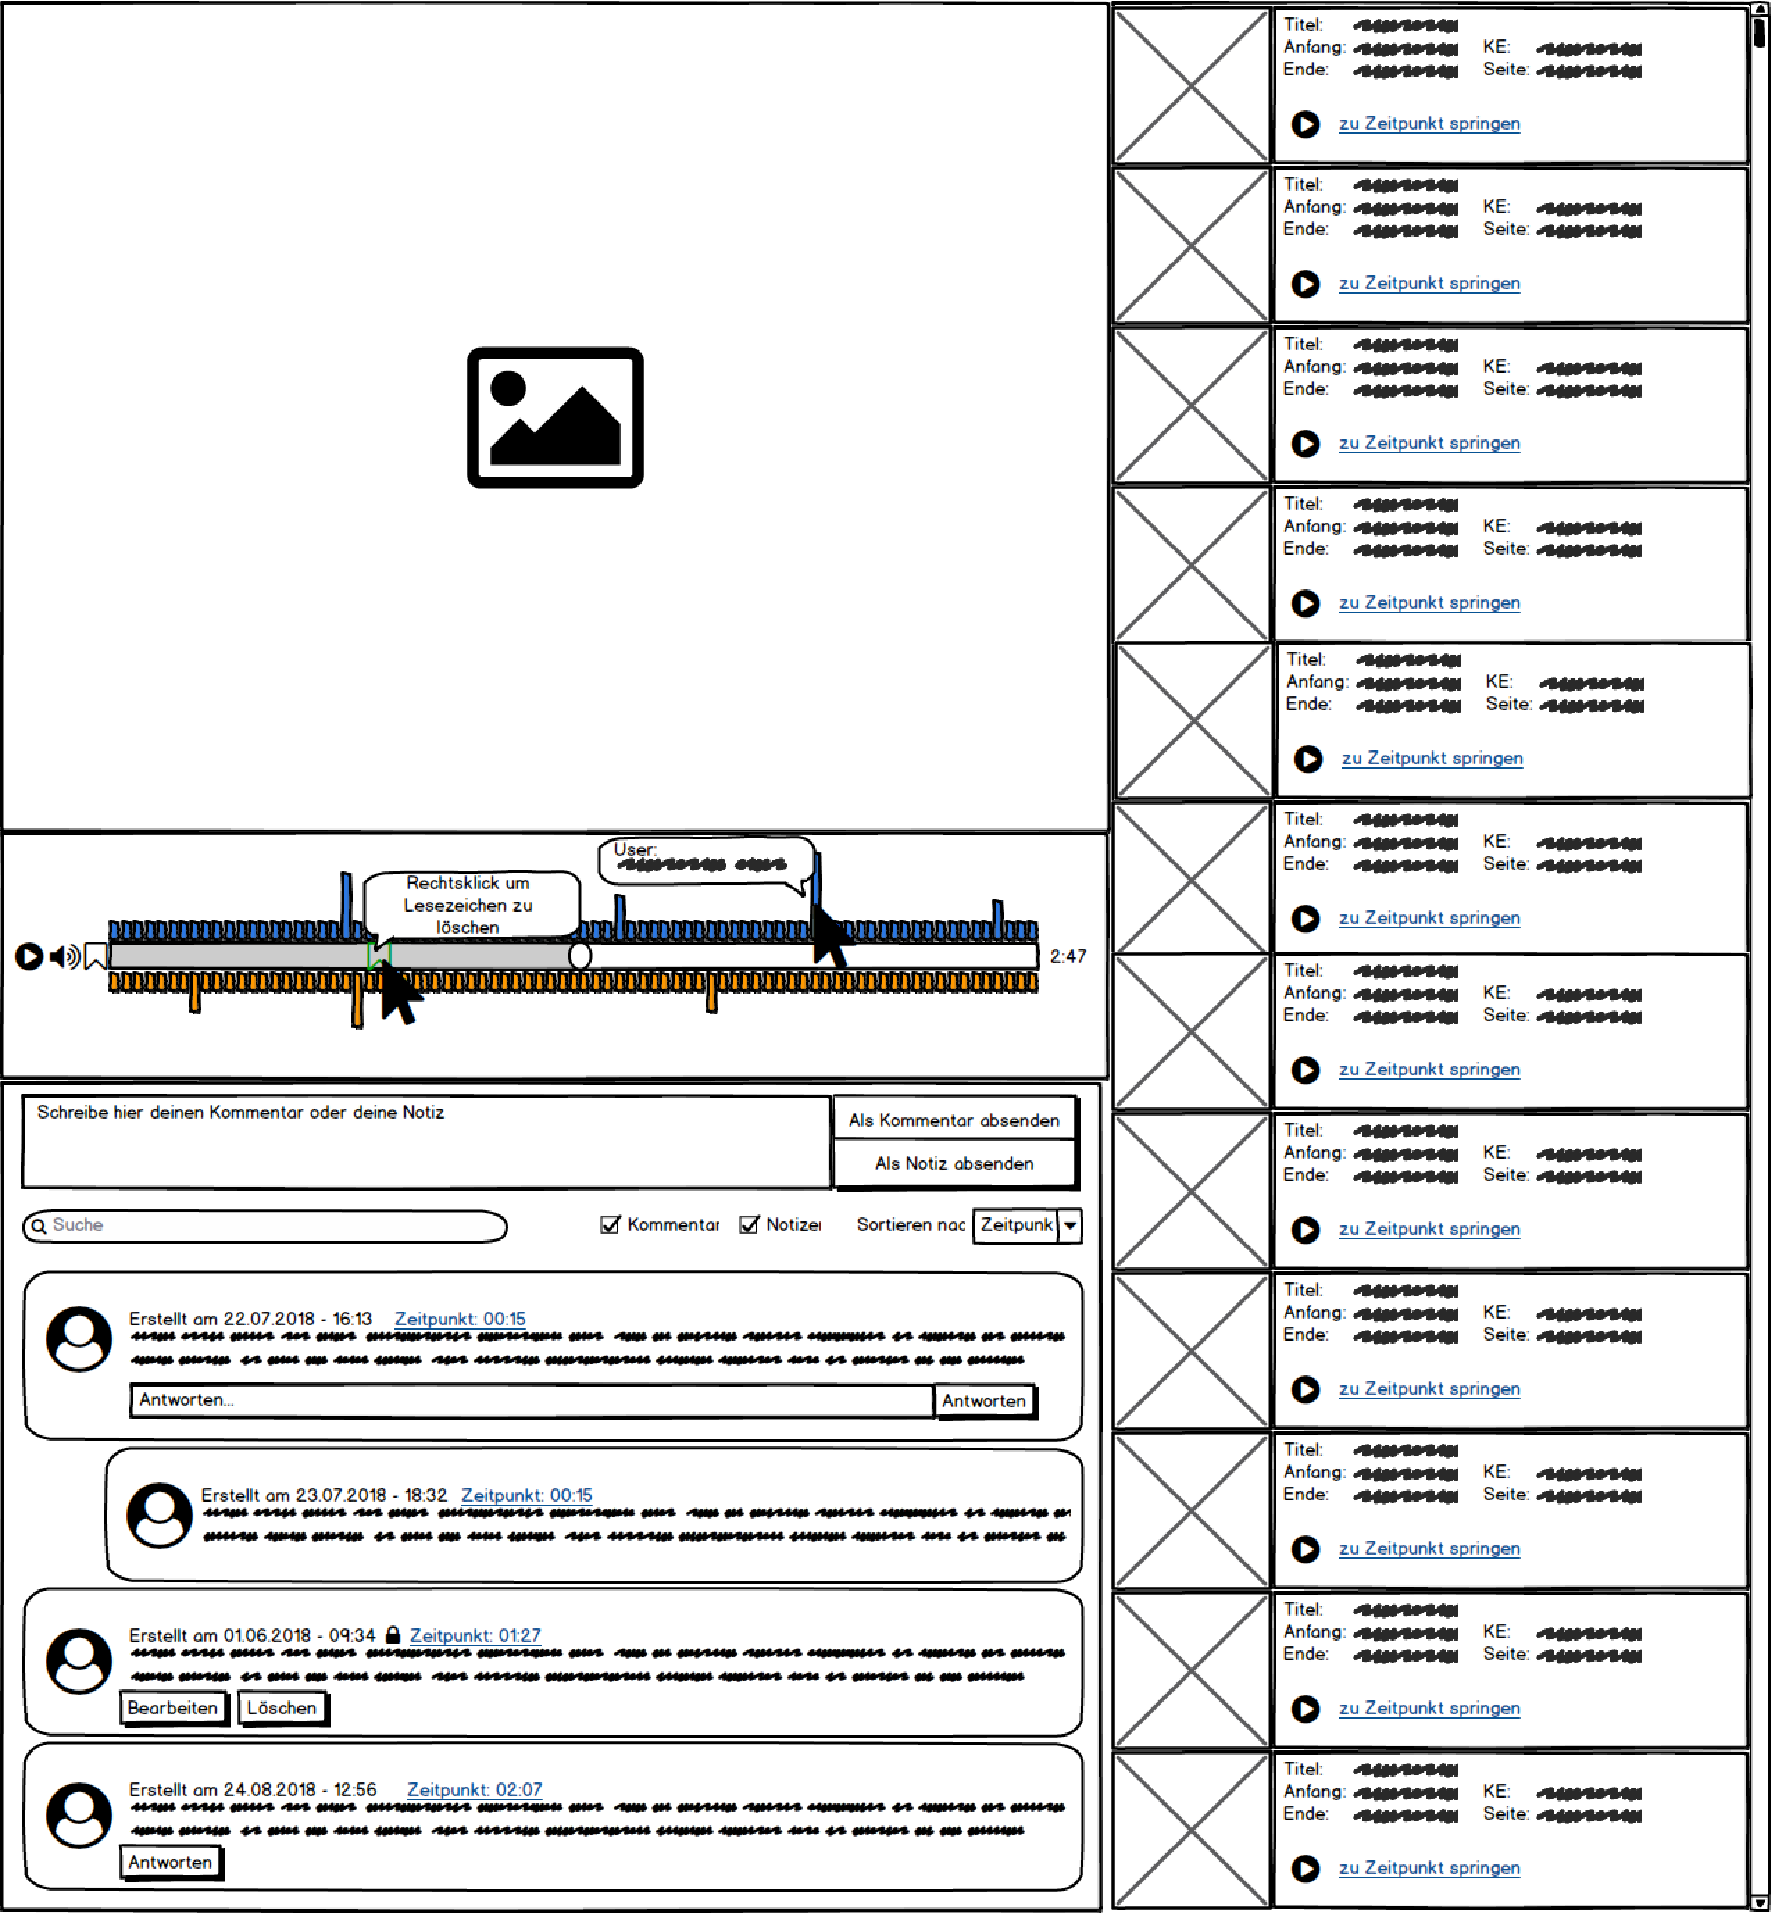
\includegraphics[width=\textwidth,center]{MockupSeiteLayoutFinal.pdf}
%\caption{\label{fig:MockupSeiteLayoutFinal}Finales Layout der Seite für Hyperaudio-Dokumente}
%\end{figure}

\begin{figure}[h!]
\begin{subfigure}[c]{\textwidth}
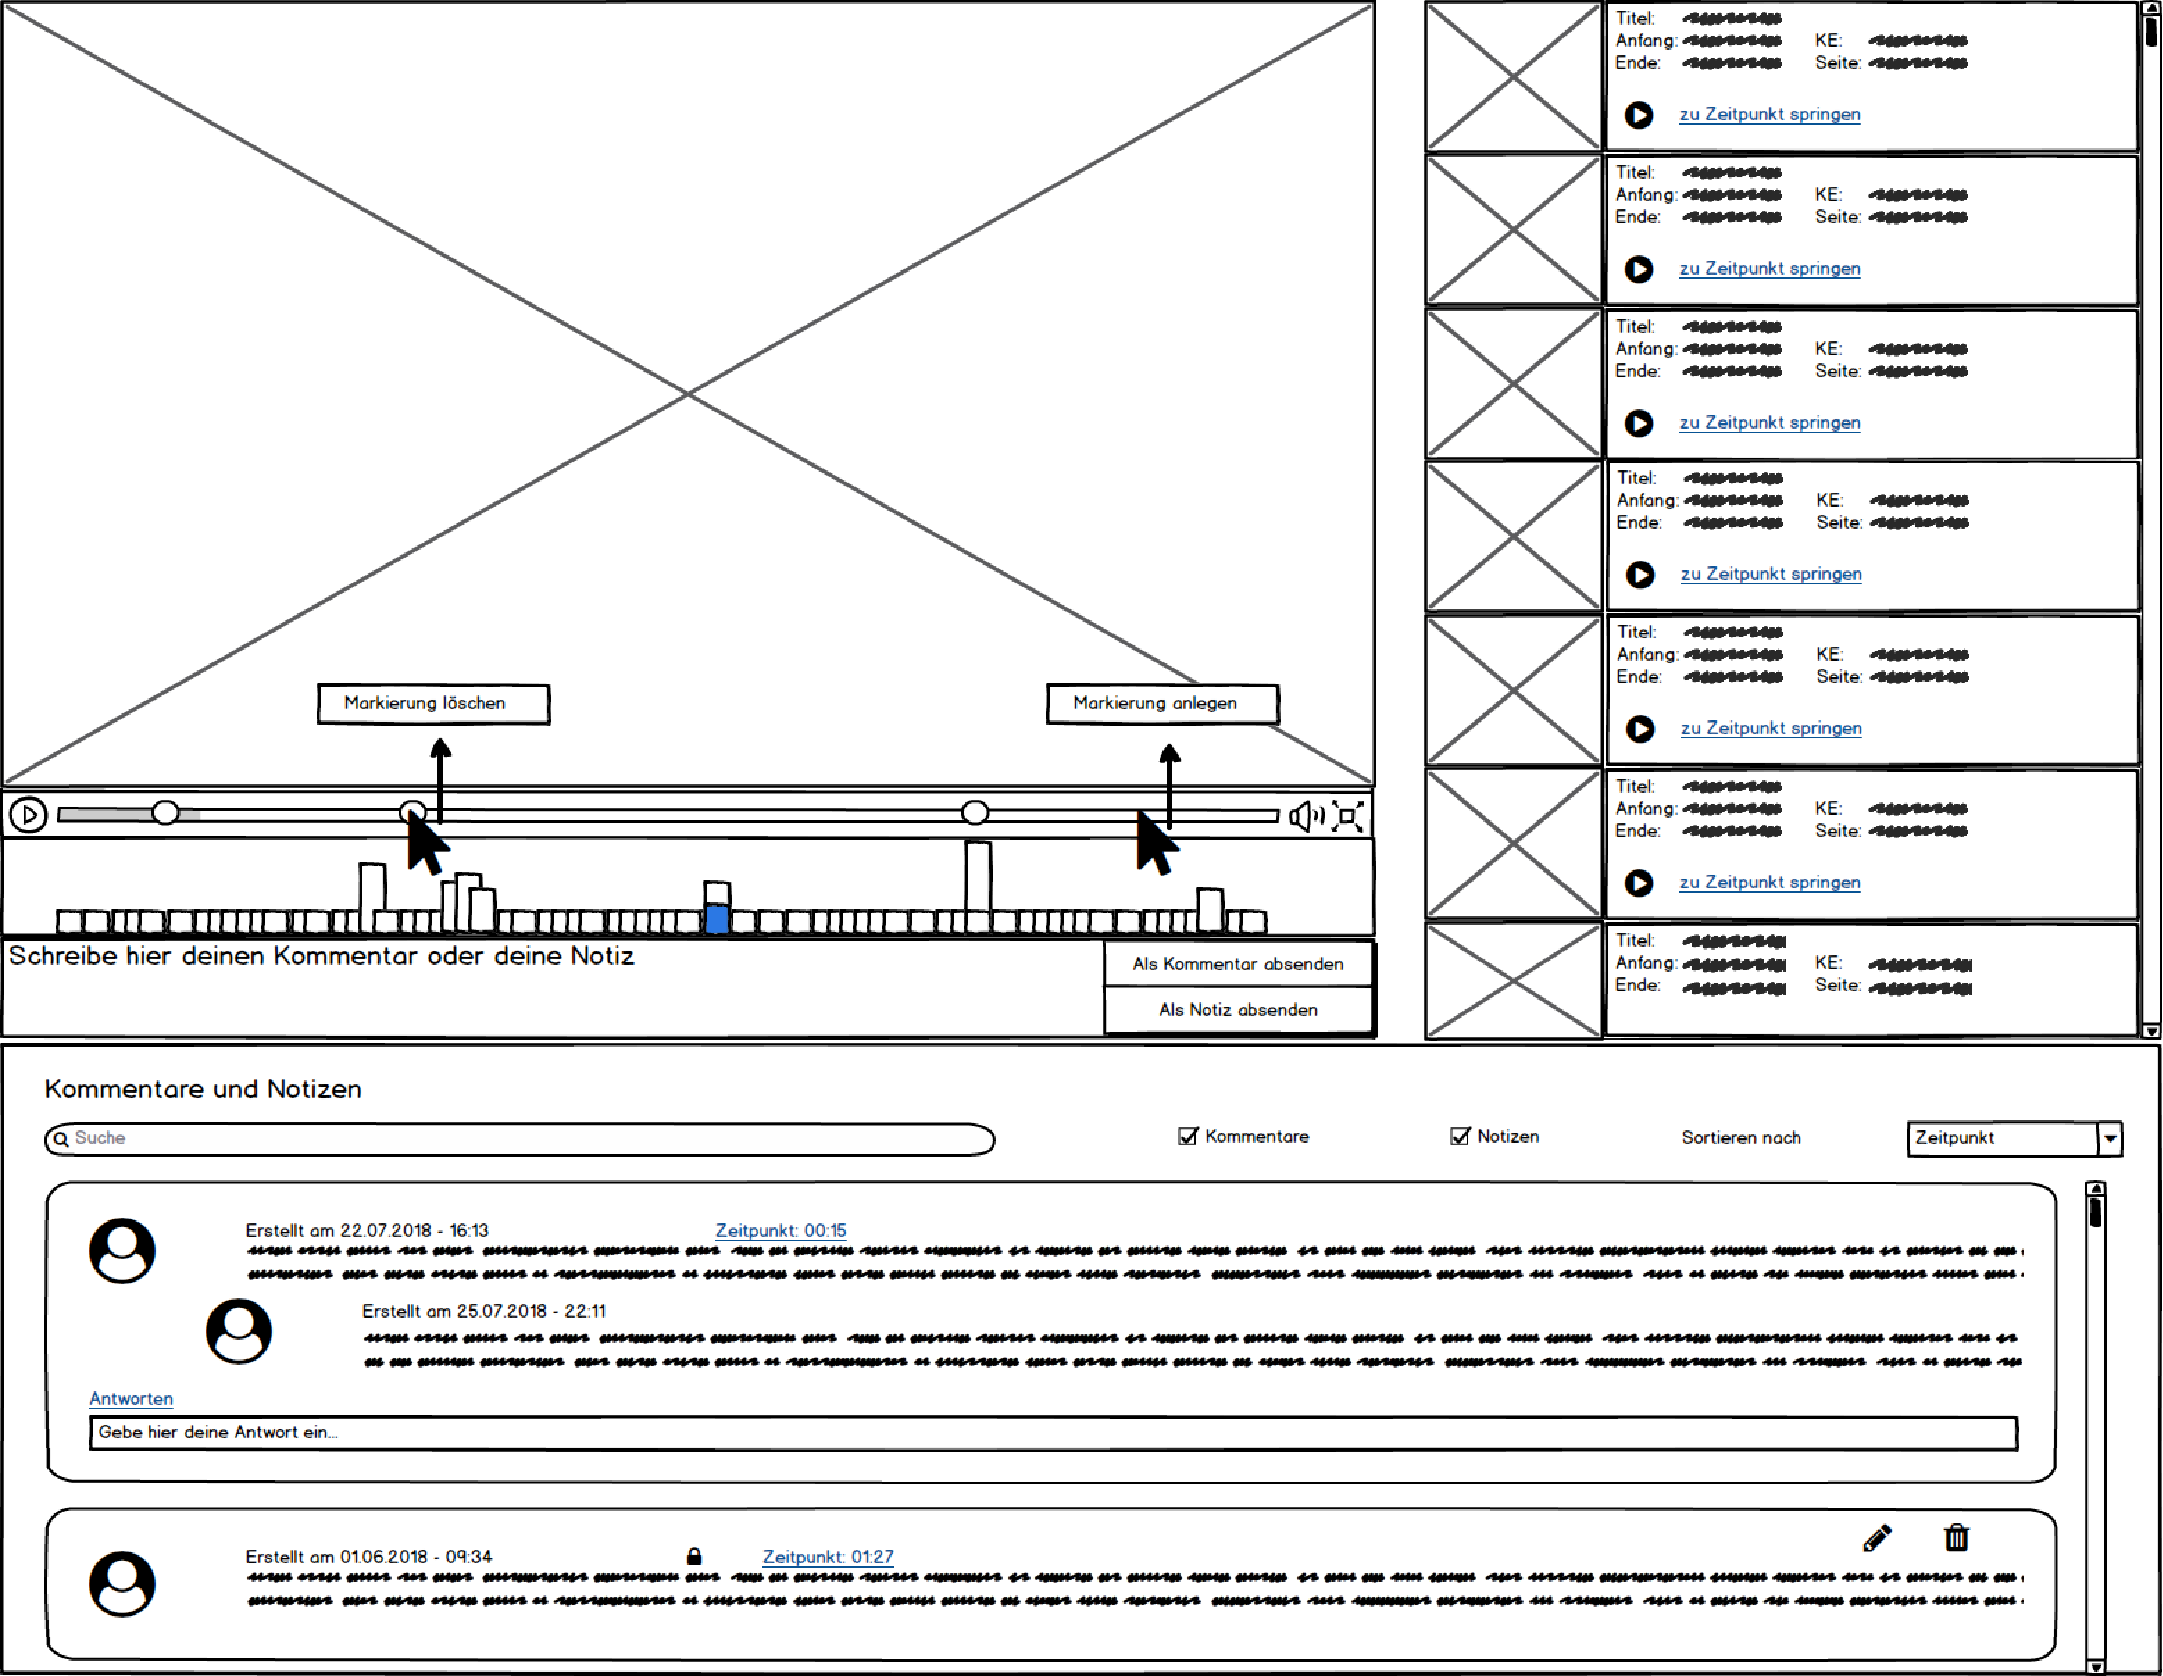
\includegraphics[width=0.9\textwidth,center]{MockupSeiteLayoutVersion1.pdf}
\subcaption{Erste Version}
\label{fig:MockupSeiteLayoutVersion1}
\end{subfigure}
\par\bigskip
\begin{subfigure}[c]{\textwidth}
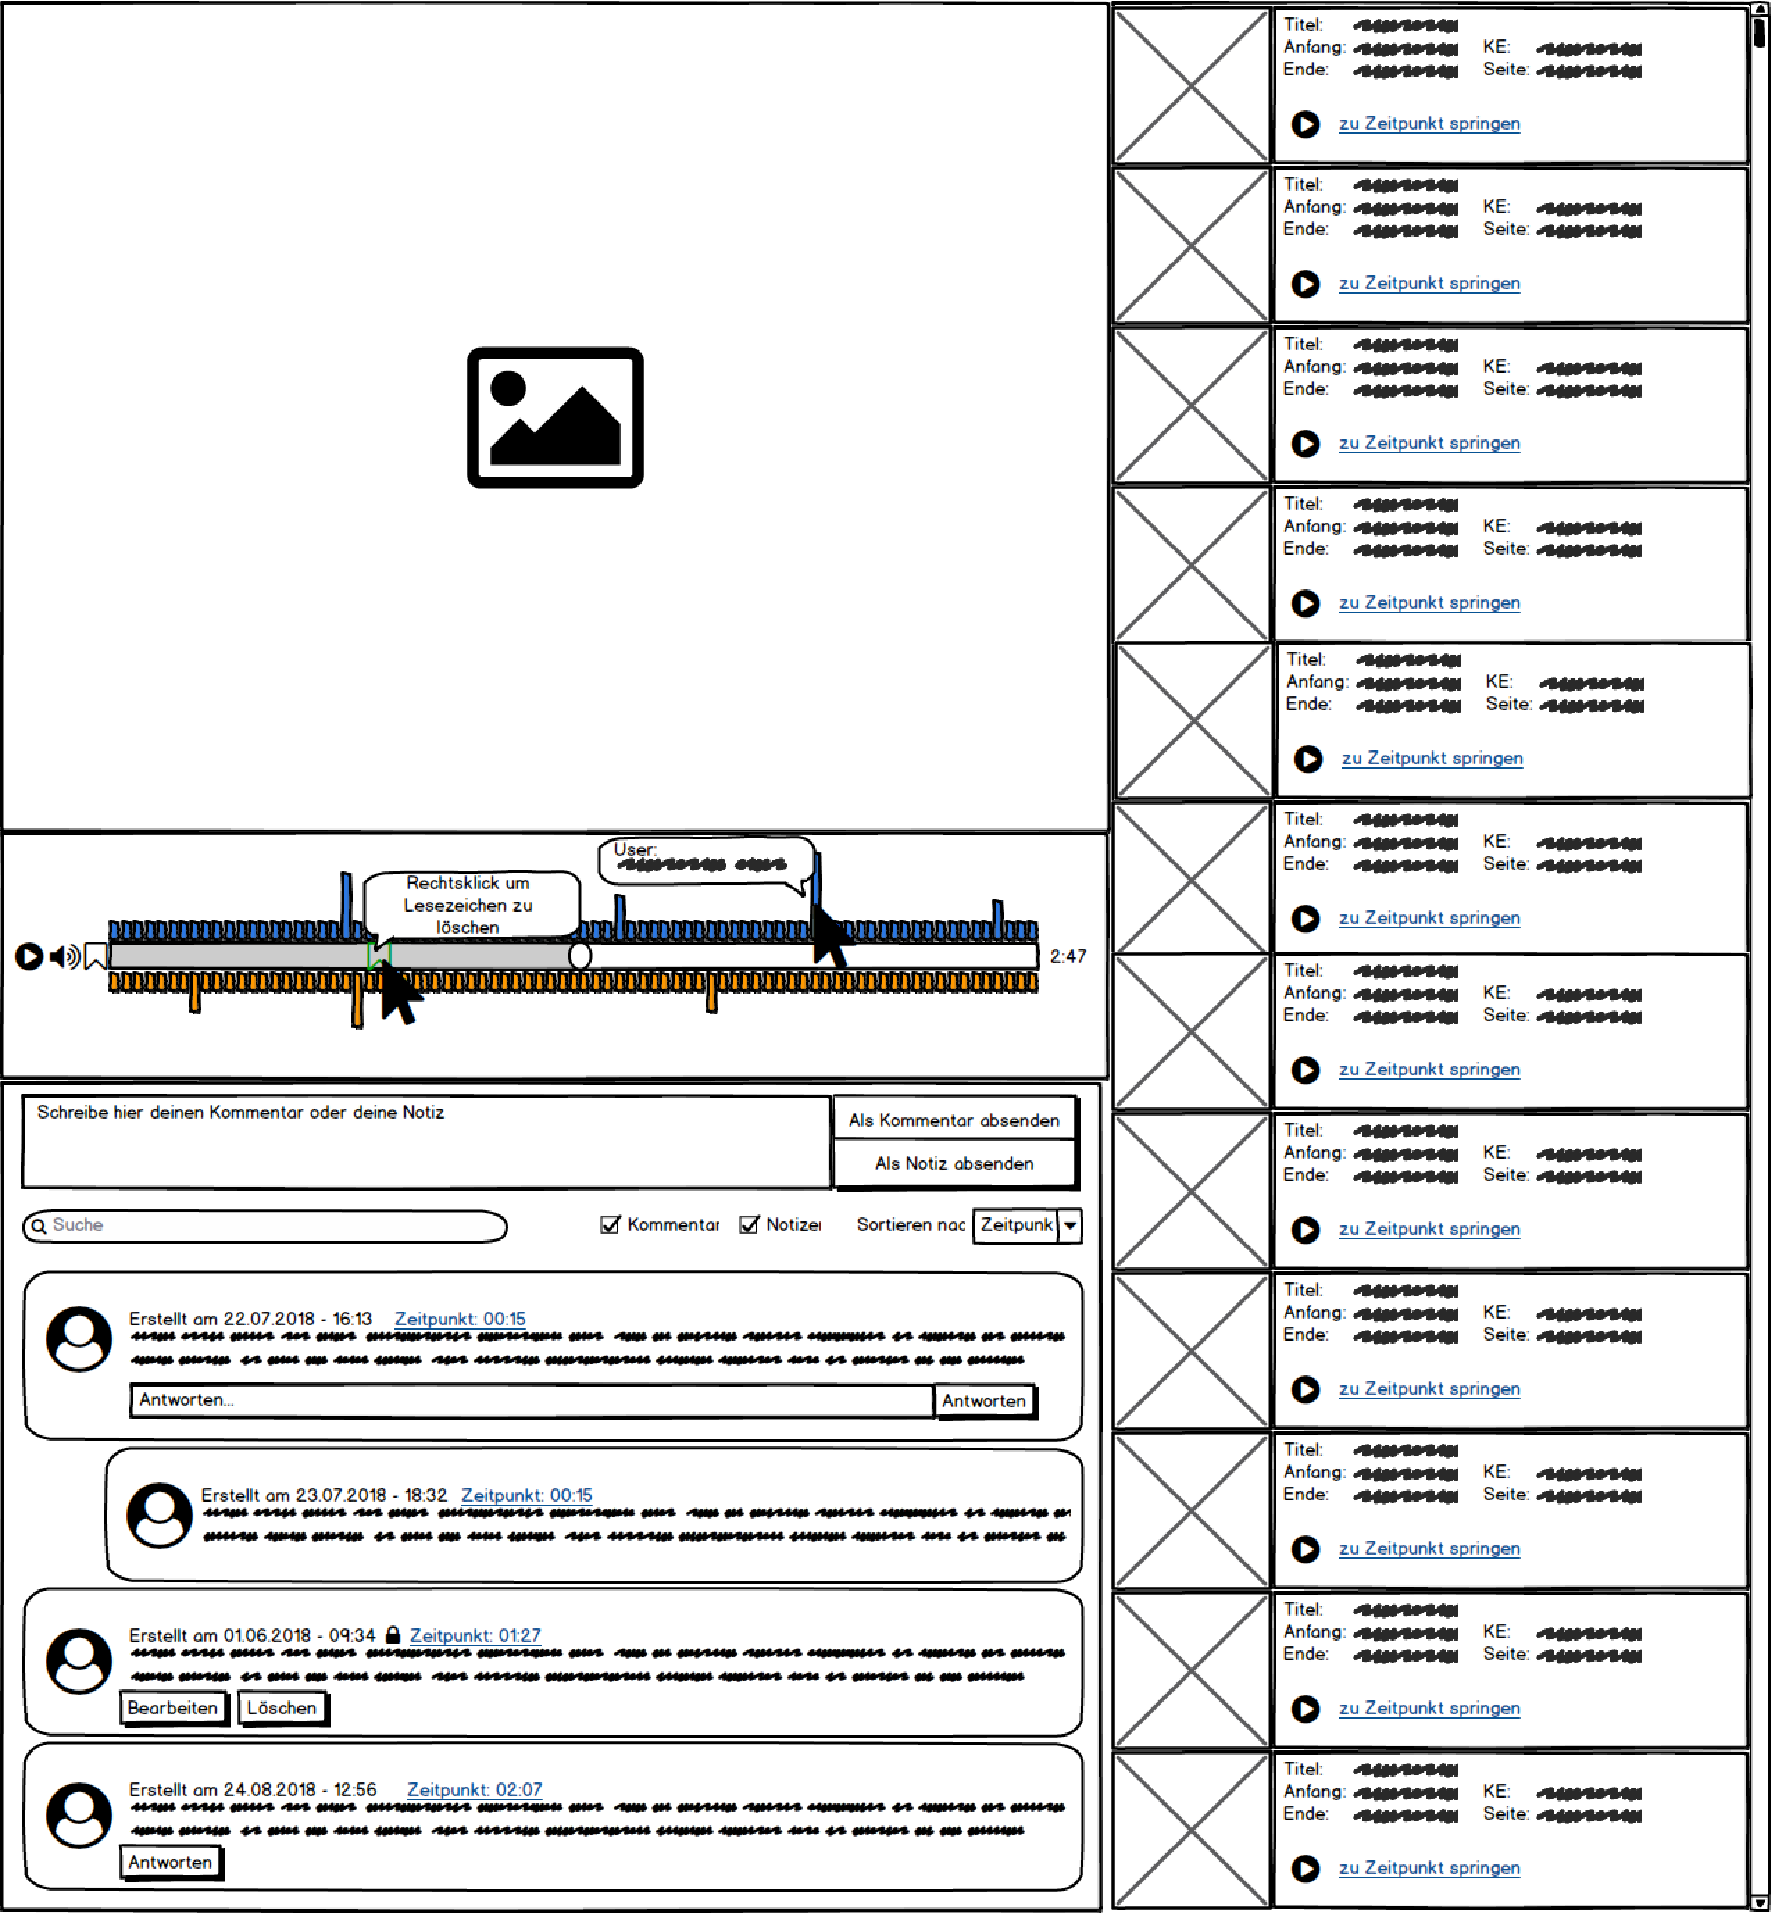
\includegraphics[width=0.9\textwidth,center]{MockupSeiteLayoutFinal.pdf}
\subcaption{Finale Version}
\label{fig:MockupSeiteLayoutFinal}
\end{subfigure}
\caption{Benutzeroberfläche - Layout der Seite für Hyperaudio-Dokumente}
\label{fig:MockupSeiteLayout}
\end{figure}

%%%%%%%%%%
%\subsection{Administrationsseite eines Hyperaudio-Dokuments}
%\dots


%%%%%%%%%%
%\subsection{Moodle-Oberfläche im Allgemeinen}
%\dots








%%%%%%%%%%
\section{Zusammenfassung}
\dots



%%%%%%%%%%%%%%%%
\chapter{Implementierung}
%% lade Kapitel aus Datei
\todo[inline]{Einleitung}

%%%%%%%%%%
\section{Architektur des Moodle-Plugins}
\label{sec:architektur}
Bei der Implementierung des Hyperaudio-Plugins ist die durch Moodle vorgegebene Architektur von Plugins zu beachten \citep{moodle2016activity}. Diese besteht stets aus vorgegebenen Dateien und Ordnen, wobei die jeweilige Anzahl von der Art des zu entwickelnden Plugins abhängig ist. Darüber hinaus bestimmt die Art des Plugins auch den zu wählenden Speicherort.

Bei Activity Plugins, wie dem Plugin für Hyperaudio-Dokumente, ist als Speicherort der Ordner \textbf{/mod} vorgeben. In diesem Ordner muss ein Unterordner mit dem Namen des Plugins angelegt werden, in diesem Fall \textbf{hyperaudio}, in welchem alle Plugin-Dateien abgelegt werden. Eine Übersicht über die Ordnerstruktur des Hyperaudio-Plugins findet sich in Abbildung \ref{fig:Ordnerstruktur}.

\begin{figure}[h!]
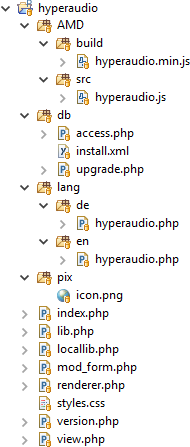
\includegraphics[width=0.3\textwidth,center]{Ordnerstruktur.PNG}
\caption{\label{fig:Ordnerstruktur}Ordnerstruktur des Hyperaudio-Plugins}
\end{figure}

\todo[inline]{Ordnerstruktur aktualisieren}

Im Ordner \textbf{/hyperaudio/backup} werden die Dateien abgelegt, welche Anwendung finden, wenn ein Backup oder eine Wiederherstellung eines Kurses vorgenommen wird.

Der Ordner \textbf{/hyperaudio/db} beherbergt die Dateien \textbf{access.php}, \textbf{events.php}, \textbf{install.xml} und \textbf{upgrade.php}. Die Datei \textbf{access.php} dient zur Steuerung der Berechtigungen innerhalb des Moodle-Plugins, wobei den verschiedenen Moodle-Rollen verschiedene Rechte für die einzelnen Funktionen zugewiesen werden können. In der \textbf{events.php} können Beobachter eingerichtet werden, welche auf bestimmte Ereignisse warten. Bei der Installation des Plugins wird die \textbf{install.xml} zur Erstellung der Datenbanktabellen für das Plugin verwendet. Es ist mindestens eine Tabelle mit dem Namen des Plugins anzulegen. Sollten die Datenbanktabellen nach Veröffentlichung des Plugins um Spalten erweitert werden, so kommt die Datei \textbf{upgrade.php} zum Einsatz. Hierin werden die notwendigen Schritte für einen Versionsabgleich definiert.

Im Ordner \textbf{/hyperaudio/lang} wird die Sprachlokalisierung vorgenommen. Für jede Sprache wird innerhalb des \textbf{lang}-Ordners ein eigener Unterordner angelegt. Darin befindet sich jeweils eine PHP-Datei, in welcher die Übersetzungen definiert werden. Der Name dieser Datei entspricht wiederum dem Namen des Plugins.

Das Icon, welches für das Plugin  verwendet werden soll, muss im Ordner \textbf{/hyperaudio/pix} mit dem Dateinamen \textbf{icon.gif} abgelegt werden und sollte eine Auflösung von 16x16 Pixel besitzen.

Im Ordner \textbf{/hyperaudio} liegen darüber hinaus die Dateien \textbf{lib.php}, \textbf{mod\underline{{ }}form.php}, \textbf{index.php}, \textbf{view.php} und \textbf{version.php}. Die \textbf{lib.php} dient dazu, Standardfunktionen von Moodle zu überschreiben, wobei \texttt{add\underline{{ }}instance}, \texttt{update\underline{{ }}instance} und \texttt{delete\underline{{ }}instance} als essenzielle Funktionen zu nennen sind. Mit diesen Funktionen wird das Anlegen, Aktualisieren und Löschen von Instanzen des Plugins ermöglicht. Zum Anlegen und Aktualisieren wird in der \textbf{mod\underline{{ }}form.php} die dazugehörige Maske festgelegt.Die \textbf{\textit{index.php}} dient der Auflistung aller Instanzen eines Plugins innerhalb eines Kurses. Je nach Umsetzung kann der Inhalt dieser Auflistung unterschiedlich viele Informationen zu den Instanzen bereitstellen. Auch ist es beispielsweise anhand von Berechtigungen aus der \textbf{access.php} möglich gewisse Inforationen nur bestimmten Usern anzuzeigen. Die erste Datei, die beim Öffnen der Aktivität geladen wird, ist die \textbf{view.php}, welche dementsprechend vornehmlich der Anzeige der Inhalte dient. In der \textbf{version.php} wird die Version des Plugins gepflegt. Erhöht sich die Versionsnummer in der \textbf{version.php}, wird der automatische Upgradeprozess von Moodle für das Plugin ausgelöst.

Neben diesen vorgegebenen Dateien kommen üblicherweise noch weitere Dateien bei der Entwicklung eines Moodle-Plugins zum Einsatz \citep{wild2017moodle}. Dazu gehört beispielsweise die \textbf{locallib.php}, in welcher üblicherweise alle plugineigenen PHP-Funktionen deklariert werden. Auch ist es Usus, die eigentliche Darstellung der Plugin-Inhalte innerhalb eines Kurses von der \textbf{view.php} in eine \textbf{renderer.php} zu verlagern. Dort können verschiedene Renderer-Klassen, welche durch Moodle bereitgestellt werden, für die eigenen Bedürfnisse überschrieben werden. Anpassungen optischer Natur können durch CSS (Cascading Style Sheets) in der \textbf{styles.css} vorgenommen werden. Eigene JavaScript-Module, welche beispielweise beim Laden der \textbf{view.php} automatisch aufgerufen werden, sind im Verzeichnis \textbf{/hyperaudio/AMD} (Asynchronous Module Definition) abzulegen.

%%%%%%%%%%
\section{Iterative Entwicklung}
Die Entwicklung des Plugins wird in iterativer Form durchgeführt. In jeder Iteration soll das Plugin nur um einige wenige Funktionalitäten erweitert werden. Jede Iteration soll mit einem lauffähigen Plugin abgeschlossen werden. So kann direkt das Ergebnis betrachtet werden und gegebenenfalls in der nächsten Iteration nochmals angepasst werden \citep{augsten2018iterativ}. Die Reihenfolge, in welcher die Funktionalitäten umgesetzt werden, leitet sich aus der Priorisierung der Anforderungen aus Abschnitt \ref{sec:anforderungsdefinition} ab.

\subsection{Speichern und Abspielen einer Audio-Datei}
In der ersten Iteration wird zunächst die grundlegende Struktur des Plugins erstellt (vgl. Abschnitt \ref{sec:architektur}). Ziel der ersten Iteration soll es sein, eine Audio-Datei speichern und wiedergeben zu können.

Dazu wird in der Maske zum Anlegen und Aktualisieren von Instanzen des Hyperaudio-Plugins (\textbf{mod\underline{{ }}form.php}) neben dem obligatorischen Namens-Feld noch ein Element zum Hinzufügen einer Audiodatei angelegt. Auflistung \ref{lst:it1:modform} zeigt einen Ausschnitt des Codes, der in der Funktion \texttt{definition} der Klasse \texttt{mod\underline{{ }}hyperaudio\underline{{ }}mod\underline{{ }}form}, die von der Klasse \texttt{moodleform\underline{{ }}mod} erbt, ergänzt werden muss. 

\begin{lstlisting}[language=php,
             linewidth=\textwidth,
             caption={Ausschnitt der \textbf{mod\underline{{ }}form.php} in der 1. Iteration},
             label={lst:it1:modform}]
$mform = $this->_form;             
$mform->addElement('text', 'name', get_string('hyperaudio_mod_form_name',
    'hyperaudio'));
$mform->setType('name', PARAM_TEXT);
$mform->addRule('name', get_string('error_wrong_hyperaudio_name_input',
    'hyperaudio'), 'required');
$mform->addElement('filemanager', 'audiofile', get_string('hyperaudiodata',
    'hyperaudio'), null,
    array(
       'subdirs' => 0,
       'maxbytes' => 0,
       'areamaxbytes' => 10485760,
       'maxfiles' => 1,
       'accepted_types' => array('audio')
    )
);
$mform->addRule('audiofile', get_string('required', 'hyperaudio'), 'required');
\end{lstlisting}

Der \texttt{\underline{{ }}form} der \texttt{moodleform\underline{{ }}mod} können durch \texttt{addElement} neue Form-Elemente hinzugefügt werden. Mithilfe der Funktionen \texttt{setType} und \texttt{addRule} können den Elementen Datentypen und Regeln zugewiesen werden, die bei Auswertung der Form automatisch validiert werden. Zum Hochladen von Dateien kann der \textit{filemanager} eingesetzt werden. Mithilfe eines Arrays können dabei Einschränkungen für Anzahl und Eigenschaften der hochzuladenden Dateien festgelegt werden. In diesem Fall darf maximal eine Datei hinzugefügt werden, die vom Typ \textit{audio} sein muss. Die Funktion \texttt{get\underline{{ }}string} dient im Allgemeinen der Darstellung der lokalisierten Bezeichnungen.

Um die Daten aus der Form in der Datenbank speichern und später wieder löschen zu können, muss auch die \textbf{lib.php} bearbeitet werden. Dazu dienen die bereits erwähnten Funktionen \texttt{add\underline{{ }}instance}, \texttt{update\underline{{ }}instance} und \texttt{delete\underline{{ }}instance}. Beispielhaft wird in Auflistung \ref{lst:it1:lib} die Funktion \texttt{add\underline{{ }}instance} zum Hinzufügen eines neuen Hyperaudio-Dokuments betrachtet. 

\begin{lstlisting}[language=php,
             linewidth=\textwidth,
             caption={Ausschnitt der \textbf{lib.php} in der 1. Iteration},
             label={lst:it1:lib}]
function hyperaudio_add_instance($data) {
    global $DB;
    
    $cmid = $data->coursemodule;
    $context = context_module::instance($cmid);
    
    $draftitemid_audiofile = $data->audiofile;
    unset($data->audiofile);
     
    $now = time();
    $data->timecreated = $now;
    $data->timemodified = $now;
    
    $data->id = $DB->insert_record('hyperaudio', $data);
    
    hyperaudio_update_audiofile($data->id, $context, $draftitemid_audiofile);
     
    return $data->id;
}
\end{lstlisting}

Der Parameter \texttt{\$data} enthält bereits die in der Form eingegebenen Daten. Das Attribut \mbox{\texttt{audiofile}} enthält nicht die Audio-Datei selbst, sondern die ID der \textit{draft file area} und soll im ersten Schritt nicht in der Tabelle \textit{hyperaudio} abgespeichert werden (vgl. Zeilen 7-8). Vor dem Speichern wird noch der aktuelle Zeitstempel hinterlegt (vgl. Zeilen 10-12). Mithilfe der Funktion \mbox{\texttt{\$DB->insert_record}} kann das \texttt{\$data}-Objekt mit seinen Attributen in der Tabelle \textit{hyperaudio} abgelegt werden. Im Nachhinein sorgt die in der \textbf{locallib.php} definierte Funktion \mbox{\texttt{hyperaudio_update_audiofile}} dafür, dass die Audio-Datei in der \textit{files}-Tabelle abgespeichert und in der \textit{hyperaudio}-Tabelle korrekt referenziert wird (vgl. Auflistung \ref{lst:it1:locallib}).

\begin{lstlisting}[language=php,
             linewidth=\textwidth,
             caption={Ausschnitt der \textbf{locallib.php} in der 1. Iteration},
             label={lst:it1:locallib}]
function hyperaudio_update_audiofile($hyperaudioid, $context, $draftitemid) {
    global $DB;
    
    file_save_draft_area_files($draftitemid, $context->id, 'mod_hyperaudio',
    'audiofile', $hyperaudioid);
    $fs = get_file_storage();
    $files = $fs->get_area_files($context->id, 'mod_hyperaudio', 'audiofile',
    $hyperaudioid, 'itemid, filepath, filename', false);

    $file = reset($files);
    $DB->set_field('hyperaudio', 'audiofile', $file->get_filename(), array(
        'id' => $hyperaudioid
    ));
}
\end{lstlisting}

Wie bereits in Abschnitt \ref{sec:architektur} angedeutet, übernimmt die \textbf{renderer.php} die Anzeige der Hyperaudio-Inhalte (siehe Auflistung \ref{lst:it1:renderer}). Die \textbf{view.php} dagegen reduziert sich auf wenige Zeilen (vgl. Auflistung \ref{lst:it1:view}). Der Plugin-Renderer wird hier benutzt, um Header, Hauptinhalte und Footer anzuzeigen.

\begin{lstlisting}[language=php,
deletekeywords={header},
             linewidth=\textwidth,
             caption={Ausschnitt der \textbf{view.php} in der 1. Iteration},
             label={lst:it1:view}]
$output = $PAGE->get_renderer('mod_hyperaudio');
echo $output->header();
echo $output->display($hyperaudio, $context);
echo $output->footer();
\end{lstlisting}

In der Funktion \texttt{display} der Klasse \mbox{\texttt{mod_hyperaudio_renderer}}, die von der Klasse \mbox{\texttt{plugin_renderer_base}} erbt, werden die HTML-Inhalte erzeugt. Dabei handelt es sich in der 1. Iteration um einen Container, der ein \texttt{<audio>}-Element beinhaltet. Als Quelle wird im \texttt{<source>}-Element eine URL (Uniform Resource Locator) angegeben, die zuvor mit Moodle-Standardmitteln erzeugt wurde und auf die in der Datenbank abgelegte Audio-Datei verweist.

\begin{lstlisting}[language=php,
             linewidth=\textwidth,
             caption={Ausschnitt der \textbf{renderer.php} in der 1. Iteration},
             label={lst:it1:renderer}]
$audio_fileinfo = array(
    'component' => 'mod_hyperaudio',
    'filearea' => 'audiofile',
    'itemid' => $hyperaudio->id,
    'contextid' => $context->id,
    'filepath' => '/',
    'filename' => $hyperaudio->audiofile
);

$audiofileurl = moodle_url::make_pluginfile_url(
    $audio_fileinfo['contextid'], $audio_fileinfo['component'],
    $audio_fileinfo['filearea'], $audio_fileinfo['itemid'],
    $audio_fileinfo['filepath'], $audio_fileinfo['filename']);
$audio_url = $audiofileurl->get_scheme() . '://' . $audiofileurl->get_host() . $audiofileurl->get_path();
if ($audiofileurl->get_port()){
    $audio_url .= ':' . $audiofileurl->get_port();
}

$output = '<div id="hyperaudio" data-hyperaudio_id="'.$hyperaudio->id.'">';
$output .= '<audio id="hyperaudio_audio" controls style="width:800px;">' .
    '<source src="' . $audio_url . '"/>' .
    '</audio>';
$output .= '</div>';

echo $output;
\end{lstlisting}

Auf die beschriebene Art und Weise lässt sich ein Hyperaudio-Dokument, das vorläufig allein aus einer Audio-Datei besteht, speichern und mithilfe des HTML5-Audio-Players wiedergeben.


\subsection{Speichern und Anzeige von Zusatzinhalten}
\dots

\subsection{Einbindung der Konfigurationsdatei}
\dots

\subsection{Speichern und Anzeige von Kommentaren}
\dots

\subsection{Antworten auf Kommentare}
\dots

\subsection{Notizen}
\dots

\subsection{Audio Cues}
\dots

\subsection{Galerie der Zusatzinhalte}
\dots

\subsection{Zeitabhängige Visualisierung der Kommentare}
\dots

\subsection{Markierungen}
\dots

%\subsection{Suche, Filter und Sortierung bei Kommentaren}
%\dots
%
%\subsection{Export-/Import-Funktion}
%\dots

%TODO: Wiedergabe von Videos

%%%%%%%%%%
\section{Zusammenfassung}
\dots



%%%%%%%%%%
\chapter{Evaluation}
%% lade Kapitel aus Datei
\label{cap:evaluation}
Nachdem die Implementierung des Hyperaudio-Plugins abgeschlossen ist, kann nun die Evaluation anhand der definierten Anforderungen und den dazugehörigen User Stories erfolgen. In diesem Zug werden analog zur Anforderungsdefinition die Bereiche unter Rücksichtnahme der Rollen Administrierende und Nutzende aufgeteilt. Innerhalb dieser beiden Bereiche wird dann analysiert in welchem Umfang die Anforderungen und User Stories durch die Implementierung erfüllt wurden. Die Reihenfolge der Analyse erfolgt unter Zuhilfenahme der festgelegten Prioritäten.

\section{Administration}
\label{sec:eval_administration}
Die Anforderungen der Administrierenden wurden in Tabelle \ref{tab:AnforderungenAdministrierenden} festgehalten.

Die erste Anforderung besteht darin Hyperaudio-Dokumente erstellen zu können. Die Erstellung von Hyperaudio-Dokumenten, wie es auch in \ref{US-Admin-Erstellen} gefordert wurde, ist durch das Hochladen einer Audio-Datei, der Zusatzinhalte sowie einer Konfigurationsdatei möglich. Somit kann diese Anforderung als erfolgreich implementiert betrachtet werden. Jedoch zeigt diese Implementierung einige Schwächen auf. So fehlt eine Validierung der Konfigurationsdatei. Dies kann zum einen damit resultieren, dass das Speichern des Hyperaudio-Dokuments fehlschlägt, wenn beispielsweise der Dateiname eines Zusatzinhaltes innerhalb der JSON-Datei falsch geschrieben wurde. Auch wird nicht sichergestellt, dass sich die Zeiträume der Zusatzinhalte nicht überschreiten. In diesem Fall werden beide Inhalte während der Überschneidung dargestellt und zerstören dabei den Aufbau der Seite. Generell wäre es wünschenswert, wenn die Erstellung von Hyperaudio-Dokumenten komplett innerhalb von Moodle über eine Art Wizzard erfolgen würde. Weitere Einschränkungen bestehen darin, dass nur eine Audio-Datei als Grundlage dienen kann und nur Bilddateien als Zusatzinhalt nutzbar sind.

Die nächste Anforderung stellt die Möglichkeit zum Bearbeiten von Hyperaudio-Dokumenten dar. Diese Anforderung wurde insofern umgesetzt, als dass es möglich ist im Nachhinein die Audio-Datei, Zusatzinhalte oder Konfigurationsdatei auszutauschen und hierüber Änderungen am Hyperaudio-Dokument vorzunehmen. Ein direkte Bearbeitung des Hyperaudio-Dokuments innerhalb von Moodle kann beim Namen und der Beschreibung erfolgen. Insofern ist eine Bearbeitung von Hyperaudio-Dokumenten möglich, diese beschränkt sich aber darauf, dass die dazugehörigen Dateien ausgetauscht werden können. Dementsprechend ist die Anforderung aus \ref{US-Admin-Bearbeiten} erfüllt, aber es treten die gleichen Nachteile wie bereits beim Erstellen auf.

Das Löschen von Hyperaudio-Dokumenten wurde vollständig implementiert, somit kann die dazugehörige Anforderung und \ref{US-Admin-Loeschen} als erfolgreich Umgesetzt betrachtet werden.

Die Export- und Import-Funktion ist nur mit den Moodle Boardmitteln umgesetzt. Es ist somit nur möglich Audio-Datei, Zusatzinhalte und Konfigurationsdatei über die Bearbeitungsmaske herunterzuladen und dann bei der Anlage eines neuen Hyperaudio-Dokuments wieder hochzuladen. Titel und Beschreibung des Hyperaudio-Dokuments müssen händisch nachgetragen werden. Hier wäre es möglich für die Zukunft eine richtige Export- und Importfunktion zu implementieren, bei welcher alle Dateien in ein Archiv gepackt werden und um eine weitere Datei für Titel und Beschreibung ergänzt werden. Dieses Archiv müsste sich dann wiederum importieren lassen können, wodurch das ganze Hyperaudio-Dokument angelegt ist.

Die gewünschten Statistiken wurden in kleinen Umfang über die \textbf{index.php} bereitgestellt. Dadurch ist es Lehrenden möglich zu sehen, wie viele Kommentare/Antworten, Notizen und Lesezeichen durch wie viele verschiedene Nutzer erstellt wurden. Es ist aber durchaus vorstellbar, dass diese Statistiken noch erweitert werden sollen. So wäre es denkbar, dass man visualisiert bekommt, welche Bereiche des Hyperaudio-Dokuments am häufigsten abgespielt wurden.

 
\section{Nutzung}
In Tabelle \ref{tab:AnforderungenNutzenden} sind die Anforderungen der Nutzenden definiert.

Als erste Anforderung wird die zum Abspielen von Hyperaudio-Dokumenten betrachtet. Durch die Implementierung wurde dieses Ziel erreicht. Es kann eine Audio-Datei abgespielt werden und zu den festgelegten Zeitpunkten wird der annotierte Zusatzinhalt dargestellt. Gleichzeitig mit der Darstellung wird auch eine Audio Cue abgespielt. Demzufolge kann neben der Anforderung an das Abspielen auch die Anforderung an die Hinweise auf Zusatzinhalte als erfüllt betrachtet werden. Hierbei trifft die bereits in Abschnitt \ref{sec:eval_administration} erwähnte Einschränkung bezüglich der Formate der Zusatzinhalte zu. Zusätzlich gibt es keine Möglichkeit die Hyperaudio-Dokumente in einen Vollbildmodus abzuspielen.


Neben dem Abspielen wurden auch den Anforderungen zum Erstellen, Anzeigen und Beantworten von Kommentaren eine hohe Priorität zugewiesen. Diesen Anforderungen wurde genüge getan, insofern alle drei Funktionalitäten gegeben sind. Dies ist ebenfalls der Fall für die Anforderung zum Erstellen, Anzeigen, Bearbeiten und Löschen persönlicher Notizen. Die Funktionalitäten wurden um eine Möglichkeit zu Rückkopplung an den Player erweitert, um den Nutzen der Funktion weiter zu erhöhen. 
\todo[inline]{wo wird gesagt, dass Löschen/Bearbeiten von Kommentaren nicht gewünscht ist}

Der Übersicht über annotierte Zusatzinhalte wurde durch die Implementierung einer Galerie für Zusatzinhalte Sorge getragen. Durch die Erweiterung der Galerie um zusätzliche Metadaten und einer Rückkopplung an den Player wurde die Funktionalität der Galerie zusätzlich über die eigentliche Anforderung hinaus erweitert.

Die Suchfunktion wurde für Kommentare als auch Notzien implementiert und findet die Kommentare und Notizen die den Suchbegriff enthalten. Somit ist die Anforderung zwar erfüllt, aber ein verbesserter Suchalgorithmus, welcher Schreibfehler verzeiht und ähnliche Wörter berücksichtigt, würde die Suche noch aufwerten.

Die Anforderung Lesezeichen setzen zu können wurde umgesetzt. Nutzende sind in der Lage Lesezeichen zu erstellen und zu löschen. 

Die gewünschte Filter- und Sortierfunktion wurde ebenso implementiert. Durch die Implementierung ist es möglich zu filtern, ob Kommentare, Notizen oder beides dargestellt werden sollen. Auch eine Sortierung nach Erstelldatum (auf- und absteigend) sowie nach Annotationszeitpunkt ist umgesetzt worden.

Es wurde eine angepasste Darstellung auf mobilen Geräten implementiert. Diese gibt dem Nutzer die Möglichkeit auch auf mobilen Endgeräten Hyperaudio-Dokumente abzuspielen, die dazugehörigen Kommentare, Notizen und Lesezeichen als auch die Galerie zu betrachten. Hierbei handelt es sich aber nur um eine angepasste Darstellung der Desktopversion. Um die Nutzung auf mobilen Geräten komfortabel zu gestalten, wäre eine komplett angepasste Darstellung der Hyperaudio-Dokumente notwendig.

Was die Anforderung in Bezug auf Favoriten und Übersicht über alle Hyperaudio-Dokumente der belegten Kurse und der zuletzt abgespielten Hyperaudio-Dokumente belangt, wurden diese bei der Implementierung nicht berücksichtigt. Nutzende können sich nur innerhalb eines Kurses einen Überblick über alle darin enthaltenen Hyperaudio-Dokumente verschaffen.

\todo[inline]{Fortsetzen}
\todo[inline]{Leere Kommentare/Notizen/Antworten}


\todo[inline]{User Stories und Anforderungen verknüpfen?}

\section{Zusammenfassung}

Durch die vorliegende Implementierung des Hyperaudio-Plugins wurden bereits viele der definierten Anforderungen erfüllt, dennoch gibt es sowohl im Bereich der Administration als auch im Bereich der Nutzung noch Verbesserungpotential. Grundsätzlich lassen sich die Fragen die \cite{mcluhan1977laws} im Zusammenhang mit seinen \textit{Tetraden der Medieneffekte} gestellt hat nach der Evaluation wie folgt beantworten:

\begin{enumerate}
\item Das Hyperaudio-Plugin erweitert Audio Vorlesungen, Podcasts und Hörbücher
\item Das Hyperaudio-Plugin macht Studienbriefe und Präsenzveranstaltungen obsolet
\item Das Hyperaudio-Plugin Bildungsradio
\item Wenn man das Hyperaudio-Plugin an seine Greznzen bringt führt dies zu Videos beziehungswiese Hypervideos
\end{enumerate}




\todo[inline]{Entwicklung von Kurseinheit zu Hyperaudio -> Rückschluss auf Tetrade der Medieneffekte}



%%%%%%%%%%%%%%%%
\chapter{Fazit}
%% lade Kapitel aus Datei
Zum Abschluss dieser Arbeit sollen die Ergebnisse nochmals zusammengefasst und der Bezug zu den anfangs gestellten Forschungsfragen hergestellt werden. Abschließend soll ein Ausblick für die Weiterentwicklung des Hyperaudio"=Plugins gegeben werden.

\section{Zusammenfassung}
Beginnend mit der Formulierung der Grundgedanken für die Repräsentation der Kurseinheiten im Hyperaudio-Format, wurde das Hyperaduio-Plugin nach einer Analyse der Anforderungen und des aktuellen Stands der Technik konzeptioniert und implementiert. Dabei stand die Beantwortung der Forschungsfragen und das Erreichen der daraus abgeleiteten Ziele im Mittelpunkt.

\begin{itemize}
\item Wie kann den Studierenden mithilfe einer Hyperaudio-Lernumgebung ermöglicht werden mehr Zeit zum Lernen nutzen zu können?
\end{itemize}

Es wurde eine zusätzliche Lernumgebung für Studierende geschaffen. Durch die Umsetzung als Moodle-Plugin ist diese nahtlos in die bestehende Infrastruktur der FernUniversität in Hagen integrierbar. Da diese Hyperaudio-Lernumgebung primär auditive Inhalte vermittelt, ist das Lernen in vielen Alltagssituationen möglich. Im Vergleich zur textuellen Repräsentation von Kurseinheiten ist nur selten die visuelle Aufmerksamkeit der Studierenden gefordert. Auf diese Notwendigkeit wird mithilfe akustischer Signale hingewiesen.

\begin{itemize}
\item Wie lassen sich auditive Inhalte verständlich gestalten?
\end{itemize}

In den Grundlagen wurden Wege aufgezeigt, wie die Vertonung von Kurseinheiten durchgeführt werden kann, sodass der Studierende den Lerninhalten erfolgreich folgen kann. Dies kann unter anderem durch den Einsatz der Prinzipien für Multimedia von \cite{mayer2009multimedia} oder unter Berücksichtigung der Erkenntnisse von \cite{donker2007gestaltung} erfolgen.

\begin{itemize}
\item Wie lassen sich Inhalte in der Hyperaudio-Lernumgebung darstellen, die nicht in auditiver Form abgebildet werden können?
\end{itemize}

Nicht auditiv repräsentierte Inhalte der Kurseinheiten, wie beispielsweise Tabellen oder Grafiken, können in Form von Bildern in die Hyperaudio-Repräsentation eingebunden werden.

\begin{itemize}
\item Wie können nicht-auditive Inhalte mit den auditiven Inhalten verknüpft werden?
\end{itemize}

Das Hyperaudio"=Plugin bietet die Möglichkeit, Bilder zu definierten Zeitpunkten darzustellen. Die Zuordnung von Bildern zu Zeitpunkten erfolgt anhand einer Konfigurationsdatei im JSON-Format. Auf die eingebundenen Zusatzinhalte wird nach dem Vorschlag von \cite{donker2007gestaltung} durch Audio Cues hingewiesen. 

\begin{itemize}
\item Wie lassen sich alle Interaktionen, die eine textuelle Darstellung der Lerninhalte bietet, in der Hyperaudio-Lernumgebung umsetzen?
\end{itemize}

In der Hyperaudio-Lernumgebung wurden Möglichkeiten geschaffen, um Interaktionen mit textuellen Kursrepräsentationen digital nachzubilden. So kann das klassische Lesezeichen in der Kurseinheit durch ein Lesezeichen in der Timeline des Hyperaudio-Dokuments ersetzt werden. Soll zudem noch eine Anmerkung notiert werden, kann statt eines Lesezeichens eine persönliche Notiz angefertigt werden. Die Galerie des Hyperaudio-Dokuments repräsentiert in gewisser Art das Inhaltsverzeichnis einer Kurseinheit sowie die Möglichkeit, durch die Seiten zu blättern. Dieses \glqq Inhaltsverzeichnis\grqq{} beinhaltet jedoch nur die visuellen, nicht aber die auditiven Inhalte. Ein vollständiges Inhaltsverzeichnis, bei dem direkt erkennbar ist, welche Themen zu welchem Zeitpunkt behandelt werden, ist nicht vorhanden.
%\todo[inline]{Sie sind hier in keiner Weise kritisch gegenüber Ihrer eigenen Arbeit. Es ist keines Falls eine perfekte Lösung, die Sie hier hingelegt haben. Es wird Ihnen auch niemand vorwerfen, Ihr eigenes Werk kritisch zu hinterfragen. Es ist vielmehr eine Frage der Haltung, den jede Kritik ist der Antrieb für eine Verbesserung und manchmal auch Innovation.}

\begin{itemize}
\item Wie kann der Austausch zwischen Studierenden und Lehrenden umgesetzt werden?
\end{itemize}
Die im Hyperaudio"=Plugin umgesetzte Kommentarfunktion ermöglicht den Austausch zwischen Studierenden und Lehrenden. Jeder Teilnehmer kann Kommentare zu bestimmten Zeitpunkten eines Hyperaudio-Dokuments verfassen oder auf bestehende Kommentare antworten. Zum jetzigen Stand gibt es jedoch keine Benachrichtigungsfunktion für neue Kommentare oder Antworten. Somit sind Studierende und Lehrende zum erneuten Aufruf der Hyperaudio"=Dokumente gezwungen, um dieses auf Neuigkeiten zu überprüfen. Die Evaluation hat ebenfalls hervorgebracht, dass die aktuelle Darstellung bei einer größeren Anzahl beziehungsweise Länge von Kommentaren, Antworten und Notizen unübersichtlich und überladen wirken kann.
%\todo[inline]{Technisch ja, praktisch aus?}
%\todo[inline]{Und? Ist die Darstellung nun gut? Gibt es Daten, die das nahelegen oder sogar bestätigen?}

Mit dem Moodle-Hyperaudio"=Plugin wurde allen zu Beginn formulierten Forschungsfragen begegnet. Dennoch ist die Entwicklung einer Hyperaudio-Lernumgebung noch nicht abgeschlossen.
%\todo[inline]{Warum? Was wurde beforscht? 
%
%Hatten Sie sich mit dem Design-Based-Research-Ansatz beschäftigt?}

\section{Ausblick}

Im Folgenden soll nun ein Ausblick für mögliche Weiterentwicklungen der Hyperaudio-Lernumgebung gegeben werden.

In der Evaluation wurde festgestellt, dass noch nicht alle Anforderungen zu voller Zufriedenheit umgesetzt wurden. Zu diesen Themen (Favoritenfunktion, Übersichten, Unterstützung mobiler Endgeräte, Fortsetzen Unterbrochener Wiedergaben und Import- und Export-Funktion) sind Nachbesserungen erforderlich. Darüber hinaus wurden bereits in Abschnitt \ref{sec:Verbesserungsvorschlaege} Verbesserungsvorschläge in Form von User Stories festgehalten.\\
Im Bezug auf \ref{US-Kommentar-Bewertung} wäre die Entwicklung einer Bewertungsfunktion für Kommentare und Antworten denkbar, wie sie beispielsweise auf der Plattform \textit{Stack Exchange}\footnote{https://stackexchange.com} zum Einsatz kommt.\\
Eine weitere Überlegung wäre es das Hyperaudio"=Plugin so zu erweitern, dass auch das Streaming auf Fernsehgeräte, zum Beispiel durch \textit{Google ChromeCast} oder \textit{Apple TV}, unterstützt wird. Hierdurch würde die Nutzung einer großen Bildschirmfläche abseits von Laptops und Desktops ermöglicht.\\
Aber auch im Bereich der kleinen Displays, also der mobilen Endgeräte, besteht noch Potenzial zur Weiterentwicklung. Es wäre eine App vorstellbar, welche neben einem speziell für mobile Geräte ausgelegten Design auch über eine Offline-Funktionalität verfügt. Damit würden die Freiheiten des Studierenden nochmals erhöht, da er beim Lernen nicht mehr abhängig von einer Internetverbindung ist.\\
Neben diesen Punkten, die sich vor allem auf die Rolle der Nutzenden beziehen, wären auch einige Weiterentwicklungen für die Administrierenden denkbar. So wäre auf lange Sicht eine Funktion von Nöten, um unerwünschte Nutzerkommentare (vgl. \cite{reinmann2002analyse}) zu löschen.\\
Für Administrierende wäre ebenfalls eine Möglichkeit zur (halb-)automatischen Konvertierung der klassischen Kurseinheiten in Hyperaudio"=Dokumente reizvoll, zum Beispiel durch den Einsatz von ScreenReadern (vgl. \cite{donker2007gestaltung}). Dies würde die Hürde zur Einführung von Hyperaudio"=Dokumenten durch die Lehrenden enorm senken, da dies mit einem wesentlich geringeren Aufwand verbunden wäre.\\
\todo[inline]{So hätte man das vor 10 Jahren gemacht. Welche Möglichkeiten gibt es heute noch?}
Eine weitere Fragestellung, die sich im Rahmen dieser Arbeit eröffnet hat, ist der Umgang mit Änderungen am Hyperaudio"=Dokument. Besonders eine Änderung der zugrundeliegenden Audio-Datei zieht weitreichende Folgen nach sich. So müssen nicht nur Zusatzinhalte und deren Annotationszeitpunkte angepasst, sondern auch bestehende Kommentare, Notizen und Lesezeichen berücksichtigt werden. In diesem Rahmen ist über eine Versionierung beziehungsweise verschiedene Optionen zum Entfernen oder Migrieren der annotierten Inhalte nachzudenken.

Diese Arbeit hat gezeigt, wie eine Hyperaudio-Lernumgebung in Moodle gestaltet werden kann. Das ausbaufähige Hyperaudio"=Plugin bietet Raum für zusätzliche Optimierungen für Nutzende als auch Administrierende.


%%%%%%%%%%%%%%%% ANHANG
\appendix

%%
\chapter{Auswertungen}
\section{Textanteil der Kurseinheiten}
\label{sec:TextanteilDerKurseinheiten}
Bei der Auswertung des Textanteils der Kurseinheiten werden exemplarisch die Kurseinheiten der Pflichtmodule eines Bachelorstudienganges Wirtschaftsinformatik\footnote{Hierbei handelt es sich um das Studium des Verfassers dieser Arbeit (WS 2014/2015 bis SS 2018), wobei die Kurseinheiten der Kurse \glqq Grundlagen der Analysis und Linearen Algebra\grqq{} und \glqq Grundzüge der Wirtschaftsinformatik\grqq{} nicht im PDF-Format vorlagen und dementsprechend bei der Analyse nicht berücksichtigt wurden.} an der FernUniversität in Hagen analysiert. Im ersten Schritt werden mithilfe des Tools \textit{PDF24 Creator 8.6.0}\footnote{https://de.pdf24.org} aus den PDF-Dokumenten alle Leerseiten, das eventuell enthaltene Glossar, alle Verzeichnisse und sonstige nicht zum eigentlichen Kurstext gehörenden Inhalte entfernt. Auch Kurseinheiten, welche selbst nur ein Glossar oder ähnliches darstellen, werden nicht berücksichtigt. Für die weitere Analyse der Kurseinheiten wird das Tool \textit{PDF-Analyzer 5.0}\footnote{https://www.is-soft.de} eingesetzt. Es werden die Seiten sowie die Wörter des Dokuments gezählt. Danach wird für jeden Kurs eine Seite mit möglichst großem Textanteil identifiziert und die Anzahl der Wörter auf dieser Seite bestimmt. Mithilfe dieser Kennzahl wird ein durchschnittlicher Textanteil pro Kurs errechnet. Durch das Verwenden eines Vergleichswerts für eine Seite, die somit einen Textanteil von 100\% aufweist, sollen Unterschiede in Schriftgröße und verwendeter Seitenfläche ausgeglichen werden.
Die Ergebnisse sind den Tabellen \ref{tab:AnalyseDerKurseinheiten} und \ref{tab:AnalyseDesTextanteilsDerKurse} zu entnehmen. Tabelle \ref{tab:AnalyseDerKurseinheiten} zeigt die Auswertung der einzelnen Kurseinheiten, während in Tabelle \ref{tab:AnalyseDesTextanteilsDerKurse} die zusammenfassende Analyse hinsichtlich des Textanteils für die Kurse dargestellt ist.

\scriptsize
\begin{longtable}{lllrrr}
\hline
Kurs & Semester & KE & Seiten & Wörter & Wörter pro Seite
\\\hline
\endhead
Algorithmische Mathematik & SS 2015 & 1 & 382 & 71.532 & 187\\
Anwendungssysteme und Geschäftsprozessmodellierung & WS 2015/2016 & 1 & 87 & 24.742 & 284\\
Anwendungssysteme und Geschäftsprozessmodellierung & WS 2015/2016 & 2 & 101 & 31.463 & 312\\
Anwendungssysteme und Geschäftsprozessmodellierung & WS 2015/2016 & 3 & 104 & 26.868 & 258\\
Betriebliche Informationssysteme & SS 2016 & 1 & 80 & 19.909 & 249\\
Betriebliche Informationssysteme & SS 2016 & 2 & 87 & 20.830 & 239\\
Betriebliche Informationssysteme & SS 2016 & 3 & 66 & 15.712 & 238\\
Betriebliche Informationssysteme & SS 2016 & 4 & 81 & 18.983 & 234\\
Betriebliche Informationssysteme & SS 2016 & 5 & 101 & 26.195 & 259\\
Betriebliche Informationssysteme & SS 2016 & 6 & 50 & 12.480 & 250\\
Betriebliche Informationssysteme & SS 2016 & 7 & 32 & 7.391 & 231\\
Buchhaltung & SS 2015 & 1 & 28 & 7.820 & 279\\
Buchhaltung & SS 2015 & 2 & 67 & 16.522 & 247\\
Buchhaltung & SS 2015 & 3 & 65 & 17.316 & 266\\
Buchhaltung & SS 2015 & 4 & 68 & 17.080 & 251\\
Buchhaltung & SS 2015 & 5 & 101 & 26.224 & 260\\
Datenbanken I & SS 2016 & 1 & 33 & 9.454 & 286\\
Datenbanken I & SS 2016 & 2 & 67 & 17.892 & 267\\
Datenbanken I & SS 2016 & 3 & 42 & 9.705 & 231\\
Datenmodellierung und Datenbanksysteme & WS 2015/2016 & 1 & 39 & 9.640 & 247\\
Datenmodellierung und Datenbanksysteme & WS 2015/2016 & 2 & 96 & 21.962 & 229\\
Datenmodellierung und Datenbanksysteme & WS 2015/2016 & 3 & 86 & 19.057 & 222\\
Datenmodellierung und Datenbanksysteme & WS 2015/2016 & 4 & 65 & 16.962 & 261\\
Einführung in das Marketing & SS 2016 & 1 & 194 & 41.166 & 212\\
Einführung in die Betriebswirtschaftslehre & WS 2014/2015 & 1 & 119 & 27.010 & 227\\
Einführung in die Betriebswirtschaftslehre & WS 2014/2015 & 2 & 102 & 26.850 & 263\\
Einführung in die Betriebswirtschaftslehre & WS 2014/2015 & 3 & 66 & 21.758 & 330\\
Einführung in die Betriebswirtschaftslehre & WS 2014/2015 & 4 & 79 & 21.412 & 271\\
Einführung in die objektorientierte Programmierung & SS 2015 & 1 & 65 & 12.723 & 196\\
Einführung in die objektorientierte Programmierung & SS 2015 & 2 & 80 & 12.079 & 151\\
Einführung in die objektorientierte Programmierung & SS 2015 & 3 & 73 & 12.146 & 166\\
Einführung in die objektorientierte Programmierung & SS 2015 & 4 & 76 & 13.359 & 176\\
Einführung in die objektorientierte Programmierung & SS 2015 & 5 & 49 & 9.039 & 184\\
Einführung in die objektorientierte Programmierung & SS 2015 & 6 & 81 & 13.267 & 164\\
Einführung in die objektorientierte Programmierung & SS 2015 & 7 & 32 & 5.326 & 166\\
Einführung in die technische und theoretische Informatik & WS 2015/2016 & 1 & 85 & 24.792 & 292\\
Einführung in die technische und theoretische Informatik & WS 2015/2016 & 2 & 69 & 23.632 & 342\\
Einführung in die technische und theoretische Informatik & WS 2015/2016 & 3 & 73 & 25.157 & 345\\
Einführung in die technische und theoretische Informatik & WS 2015/2016 & 4 & 104 & 33.712 & 324\\
Einführung in die Volkswirtschaftslehre & WS 2014/2015 & 1 & 106 & 25.320 & 239\\
Einführung in die Volkswirtschaftslehre & WS 2014/2015 & 2 & 95 & 19.589 & 206\\
Einführung in die Volkswirtschaftslehre & WS 2014/2015 & 3 & 53 & 17.519 & 331\\
Finanzierung & WS 2015/2016 & 1 & 127 & 36.003 & 283\\
Finanzierung & WS 2015/2016 & 2 & 165 & 43.454 & 263\\
Grundbegriffe und Systeme der Kosten- und Leistungsrechnung & SS 2016 & 1 & 155 & 33.884 & 219\\
Grundbegriffe und Systeme der Kosten- und Leistungsrechnung & SS 2016 & 2 & 120 & 28.329 & 236\\
Grundlagen der Leistungserstellung & SS 2016 & 1 & 50 & 11.358 & 227\\
Grundlagen der Leistungserstellung & SS 2016 & 2 & 90 & 15.351 & 171\\
Grundlagen der Statistik & WS 2014/2015 & 1 & 153 & 19.647 & 128\\
Grundlagen der Statistik & WS 2014/2015 & 2 & 151 & 20.236 & 134\\
Grundlagen der Statistik & WS 2014/2015 & 3 & 110 & 15.995 & 145\\
Grundzüge der betrieblichen Steuerlehre & SS 2015 & 1 & 86 & 25.705 & 299\\
Informationsmanagement & WS 2017/2018 & 1 & 92 & 27.716 & 301\\
Informationsmanagement & WS 2017/2018 & 2 & 91 & 28.632 & 315\\
Informationsmanagement & WS 2017/2018 & 3 & 111 & 33.975 & 306\\
Informationsmanagement & WS 2017/2018 & 4 & 101 & 28.896 & 286\\
Informationsmanagement & WS 2017/2018 & 5 & 50 & 15.151 & 303\\
Informationsmanagement & WS 2017/2018 & 6 & 60 & 19.835 & 331\\
Investition & WS 2015/2016 & 1 & 72 & 18.779 & 261\\
Investition & WS 2015/2016 & 2 & 94 & 21.330 & 227\\
Investition & WS 2015/2016 & 3 & 63 & 13.407 & 213\\
Investition & WS 2015/2016 & 4 & 98 & 19.090 & 195\\
Investition & WS 2015/2016 & 5 & 99 & 21.603 & 218\\
Jahresabschluss & SS 2015 & 1 & 83 & 14.387 & 173\\
Jahresabschluss & SS 2015 & 2 & 98 & 19.007 & 194\\
Jahresabschluss & SS 2015 & 3 & 142 & 24.159 & 170\\
Jahresabschluss & SS 2015 & 4 & 115 & 26.581 & 231\\
Objektorientierte Systemanalyse & WS 2015/2016 & 1 & 103 & 32.447 & 315\\
Objektorientierte Systemanalyse & WS 2015/2016 & 2 & 185 & 48.088 & 260\\
Sicherheit im Internet I & SS 2016 & 1 & 47 & 16.321 & 347\\
Sicherheit im Internet I & SS 2016 & 2 & 62 & 19.917 & 321\\
Sicherheit im Internet I & SS 2016 & 3 & 54 & 16.421 & 304\\
Sicherheit im Internet I & SS 2016 & 4 & 48 & 16.011 & 334\\
Theorie der Marktwirtschaft & WS 2016/2017 & 1 & 54 & 19.168 & 355\\
Theorie der Marktwirtschaft & WS 2016/2017 & 2 & 214 & 57.132 & 267\\
Theorie der Marktwirtschaft & WS 2016/2017 & 3 & 141 & 31.494 & 223\\
Theorie der Marktwirtschaft & WS 2016/2017 & 4 & 185 & 47.198 & 255\\
Theorie der Marktwirtschaft & WS 2016/2017 & 5 & 69 & 19.168 & 278\\
\caption{Auswertung der Kurseinheiten}
\label{tab:AnalyseDerKurseinheiten}
\end{longtable}
\normalsize

\begin{sidewaystable}
\resizebox{\textwidth}{!}{%
\begin{tabular}{lllrrrrr}
\hline
Modul & Fakultät & Kurs & \multicolumn{1}{p{3.5cm}}{\raggedleft Wörter auf Seite mit maximalem Inhalt} & Seiten & Wörter & \multicolumn{1}{p{2cm}}{\raggedleft Wörter \\ pro Seite} & Textanteil
\\\hline
Algorithmische Mathematik & Fakultät für Mathematik und Informatik & Algorithmische Mathematik & 316 & 382 & 71532 & 187 & 59,26\%\\
Betriebliche Informationssysteme & Fakultät für Mathematik und Informatik & Betriebliche Informationssysteme & 400 & 497 & 121500 & 244 & 61,12\%\\
Einführung in die objektorientierte Programmierung & Fakultät für Mathematik und Informatik & Einführung in die objektorientierte Programmierung & 370 & 456 & 77939 & 171 & 46,19\%\\
Einführung in die technischen und theoretischen Grundlagen der Informatik & Fakultät für Mathematik und Informatik & Einführung in die technische und theoretische Informatik & 409 & 331 & 107293 & 324 & 79,25\%\\
Einführung in Internet-Technologien und Informationssysteme & Fakultät für Mathematik und Informatik & Datenbanken I & 462 & 142 & 37051 & 261 & 56,48\%\\
Einführung in Internet-Technologien und Informationssysteme & Fakultät für Mathematik und Informatik & Sicherheit im Internet I & 458 & 211 & 68670 & 325 & 71,06\%\\
Einführung in die Wirtschaftswissenschaft & Fakultät für Wirtschaftswissenschaft & Einführung in die Betriebswirtschaftslehre & 381 & 366 & 97030 & 265 & 69,58\%\\
Einführung in die Wirtschaftswissenschaft & Fakultät für Wirtschaftswissenschaft & Einführung in die Volkswirtschaftslehre & 398 & 254 & 62428 & 246 & 61,75\%\\
Externes Rechnungswesen & Fakultät für Wirtschaftswissenschaft & Buchhaltung & 374 & 329 & 84962 & 258   & 69,05\%\\
Externes Rechnungswesen & Fakultät für Wirtschaftswissenschaft & Grundzüge der betrieblichen Steuerlehre & 445 & 86 & 25705 & 299 & 67,17\%\\
Externes Rechnungswesen & Fakultät für Wirtschaftswissenschaft & Jahresabschluss & 301 & 438 & 84134 & 192 & 63,82\%\\
Grundlagen der Wirtschaftsmathematik und Statistik & Fakultät für Wirtschaftswissenschaft & Grundlagen der Statistik & 239 & 414 & 55878 & 135 & 56,47\%\\
Informationsmanagement & Fakultät für Wirtschaftswissenschaft & Informationsmanagement & 429 & 505 & 154205 & 305 & 71,18\%\\
Internes Rechnungswesen und funktionale Steuerung & Fakultät für Wirtschaftswissenschaft & Einführung in das Marketing & 292 & 194 & 41166 & 212 & 72,67\%\\
Internes Rechnungswesen und funktionale Steuerung & Fakultät für Wirtschaftswissenschaft & Grundbegriffe und Systeme der Kosten- und Leistungsrechnung & 385 & 275 & 62213 & 226 & 58,76\%\\
Internes Rechnungswesen und funktionale Steuerung & Fakultät für Wirtschaftswissenschaft & Grundlagen der Leistungserstellung & 353 & 140 & 26709 & 191 & 54,04\%\\
Investition und Finanzierung & Fakultät für Wirtschaftswissenschaft & Finanzierung & 405 & 292 & 79457 &  272 & 67,19\%\\
Investition und Finanzierung & Fakultät für Wirtschaftswissenschaft & Investition & 395 & 426 & 94209 & 221 & 55,99\%\\
Modellierung von Informationssystemen & Fakultät für Wirtschaftswissenschaft & Anwendungssysteme und Geschäftsprozessmodellierung & 429 & 292 & 83073 & 284 & 66,32\%\\
Modellierung von Informationssystemen & Fakultät für Wirtschaftswissenschaft & Datenmodellierung und Datenbanksysteme & 419 & 286 & 67621 & 236 & 56,43\%\\
Modellierung von Informationssystemen & Fakultät für Wirtschaftswissenschaft & Objektorientierte Systemanalyse & 399 & 288 & 80535 & 280 & 70,08\%\\
Theorie der Marktwirtschaft (Mikroökonomik) & Fakultät für Wirtschaftswissenschaft & Theorie der Marktwirtschaft & 403 & 663 & 174160 & 263 & 65,18\%\\
\end{tabular}}
\caption{Analyse des Textanteils der Kurse}
\label{tab:AnalyseDesTextanteilsDerKurse}
\end{sidewaystable}


Zusammenfassend wird ein nach Seitenzahl gewichteter Durchschnitt über den Textanteil gebildet. Dieser liegt bei 63,36\%. Die Standardabweichung beträgt 7,51 Prozentpunkte. Getrennt nach Fakultät ergibt sich ein durchschnittlicher Textanteil von 61,08\% an der Fakultät für Mathematik und Informatik mit einer Standardabweichung von 10,61 Prozentpunkten und ein durchschnittlicher Textanteil von 64,24\% an der Fakultät für Wirtschaftswissenschaften mit einer Standardabweichung von 6,36 Prozentpunkten. Diese Ergebnisse gelten natürlich nur für die exemplarisch gewählten Kurseinheiten.

Es ist anzumerken, dass bei dieser Herangehensweise folgende Punkte die Auswertung verfälschen:
\begin{itemize}
\item Nicht jede Fläche, die nicht durch Text in Anspruch genommen wird, enthält automatisch einen anderen visuellen Inhalt. So sollte beispielsweise eine Seite mit wenigen Zeilen Text und einer großen Abbildung mit niedrigem Textanteil in die Auswertung eingehen, während die letzte Seite eines Kapitels, auf der nur noch wenige Zeilen Text stehen, mit einem hohen Textanteil in die Auswertung eingehen sollten.
\item Formeln, Tabellen und Code-Beispiele werden ebenfalls als Text interpretiert. Hier wäre im Einzelfall zu entscheiden, ob diese Bestandteile als Text gewertet werden sollen oder nicht.
\item Die Formatierung der Inhalte beeinflusst die Auswertung dahingehend, dass beim Einsatz vieler Überschriften, Einrückungen oder Aufzählungen der ermittelte Textanteil geringer ausfällt.
\item Die Ergebnisse hängen stark von der gewählten Vergleichsseite ab.
\end{itemize}

Anhand der durchgeführten Auswertung kann ein Eindruck über die Verteilung zwischen Text und nicht-textuellen Inhalten in Kurseinheiten gewonnen werden. Um verlässliche Zahlen zu generieren, wären intensivere Studien nötig.

\FloatBarrier

\section{Einsatz von Moodle}
\label{sec:EinsatzVonMoodle}
Tabelle \ref{tab:VerwendungVonMoodle} zeigt die Auflistung der Pflichtmodule des Bachelorstudiengangs Wirtschaftsinformatik mit der Information, ob Moodle in den Kursen eingesetzt wird.


\begin{sidewaystable}
\resizebox{\textwidth}{!}{%
\begin{tabular}{lllrrrrr}
\hline
Modul & Fakultät & Kurs & Moodle im Einsatz
\\\hline
Algorithmische Mathematik & Fakultät für Mathematik und Informatik & Algorithmische Mathematik & nein\\
Betriebliche Informationssysteme & Fakultät für Mathematik und Informatik & Betriebliche Informationssysteme & nein\\
Einführung in die objektorientierte Programmierung & Fakultät für Mathematik und Informatik & Einführung in die objektorientierte Programmierung & nein\\
Einführung in die technischen und theoretischen Grundlagen der Informatik & Fakultät für Mathematik und Informatik & Betriebssysteme und Rechnernetze für Wirtschaftsinformatiker & nein\\
Einführung in die technischen und theoretischen Grundlagen der Informatik & Fakultät für Mathematik und Informatik & Einführung in die technische und theoretische Informatik & nein\\
Einführung in Internet-Technologien und Informationssysteme & Fakultät für Mathematik und Informatik & Daten- und Dokumentenmanagement im Internet & nein\\
Einführung in Internet-Technologien und Informationssysteme & Fakultät für Mathematik und Informatik & Datenbanken I & nein\\
Einführung in Internet-Technologien und Informationssysteme & Fakultät für Mathematik und Informatik & Einführung in wissensbasierte Systeme & nein\\
Einführung in Internet-Technologien und Informationssysteme & Fakultät für Mathematik und Informatik & Sicherheit im Internet I & nein\\
Einführung in die Wirtschaftsinformatik & Fakultät für Wirtschaftswissenschaft & Einführung in die Wirtschaftsinformatik & ja\\
Einführung in die Wirtschaftswissenschaft & Fakultät für Wirtschaftswissenschaft & Einführung in die Betriebswirtschaftslehre & ja\\
Einführung in die Wirtschaftswissenschaft & Fakultät für Wirtschaftswissenschaft & Einführung in die Volkswirtschaftslehre & ja\\
Externes Rechnungswesen & Fakultät für Wirtschaftswissenschaft & Buchhaltung & ja\\
Externes Rechnungswesen & Fakultät für Wirtschaftswissenschaft & Grundzüge der betrieblichen Steuerlehre & ja\\
Externes Rechnungswesen & Fakultät für Wirtschaftswissenschaft & Jahresabschluss & ja\\
Grundlagen der Wirtschaftsmathematik und Statistik & Fakultät für Wirtschaftswissenschaft & Grundlagen der Analysis und Linearen Algebra & ja\\
Grundlagen der Wirtschaftsmathematik und Statistik & Fakultät für Wirtschaftswissenschaft & Grundlagen der Statistik & ja\\
Informationsmanagement & Fakultät für Wirtschaftswissenschaft & Informationsmanagement & ja\\
Internes Rechnungswesen und funktionale Steuerung & Fakultät für Wirtschaftswissenschaft & Einführung in das Marketing & ja\\
Internes Rechnungswesen und funktionale Steuerung & Fakultät für Wirtschaftswissenschaft & Grundbegriffe und Systeme der Kosten- und Leistungsrechnung & ja\\
Internes Rechnungswesen und funktionale Steuerung & Fakultät für Wirtschaftswissenschaft & Grundlagen der Leistungserstellung & ja\\
Investition und Finanzierung & Fakultät für Wirtschaftswissenschaft & Finanzierung & ja\\
Investition und Finanzierung & Fakultät für Wirtschaftswissenschaft & Investition & ja\\
Makroökonomik & Fakultät für Wirtschaftswissenschaft & Makroökonomik I (Dateikurs und Studienbrief) & ja\\
Makroökonomik & Fakultät für Wirtschaftswissenschaft & Makroökonomik II (Dateikurs und Studienbrief) & ja\\
Modellierung von Informationssystemen & Fakultät für Wirtschaftswissenschaft & Anwendungssysteme und Geschäftsprozessmodellierung & ja\\
Modellierung von Informationssystemen & Fakultät für Wirtschaftswissenschaft & Datenmodellierung und Datenbanksysteme & ja\\
Modellierung von Informationssystemen & Fakultät für Wirtschaftswissenschaft & Grundlagen der Modellierung betrieblicher Informationssysteme & ja\\
Modellierung von Informationssystemen & Fakultät für Wirtschaftswissenschaft & Objektorientierte Systemanalyse & ja\\
Theorie der Marktwirtschaft (Mikroökonomik) & Fakultät für Wirtschaftswissenschaft & Theorie der Marktwirtschaft & ja\\

\end{tabular}}
\caption{Verwendung von Moodle in den Pflichtmodulen des Bachelorstudiengangs Wirtschaftsinformatik (Sommersemester 2018)}
\label{tab:VerwendungVonMoodle}
\end{sidewaystable}
\end{sloppypar}

%%
%\chapter{Zweiter Teil des Anhangs}
%\dots




%%% Verzeichnisse
\backmatter
\pagestyle{fancyclear}



%% Literaturverzeichnis
%\phantomsection\addcontentsline{toc}{chapter}{Literaturverzeichnis}
{\footnotesize\flushleft\setlength{\itemsep}{-3pt}%\setlength{\bibsep}{3pt}
\bibliographystyle{plainnat}
\bibliography{literatur}}
\cleardoublepage


%% Abbildungsverzeichnis
\phantomsection\addcontentsline{toc}{chapter}{Abbildungsverzeichnis}
\listoffigures
\cleardoublepage


%% Tabellenverzeichnis
\phantomsection\addcontentsline{toc}{chapter}{Tabellenverzeichnis}
\listoftables
\cleardoublepage


%% Auflistungsverzeichnis
\phantomsection\addcontentsline{toc}{chapter}{Auflistungsverzeichnis}
\renewcommand\lstlistlistingname{Verzeichnis der Auflistungen}
\lstlistoflistings
\cleardoublepage


%% Verzeichnis von Algorithmen
%\phantomsection\addcontentsline{toc}{chapter}{Verzeichnis der Algorithmen}
%\renewcommand*\listalgorithmcfname{Verzeichnis der Algorithmen}
%\listofalgorithms
%\cleardoublepage


%% Abkürzungsverzeichnis
\phantomsection\addcontentsline{toc}{chapter}{Abkürzungsverzeichnis}
\chapter*{Abkürzungsverzeichnis}

%\begin{description}
%\item[AJAX] Asynchronous JavaScript and XML
%\item[API] Application Programing Interface
%\item[BMBF] Bundesministerium für Bildung und Forschung
%\item[JSON] JavaScript Object Notation
%\item[Moodle] Modular Object-Oriented Dynamic Learning Environment
%\item[XML] Extensible Markup Language
%\end{description}

\renewcommand*{\arraystretch}{1.4}
\setlength{\LTleft}{0pt}
\begin{longtable}[l]{p{2cm}p{15cm}}
\textbf{AJAX} & Asynchronous JavaScript and XML \\
\textbf{AMD} & Asynchronous Module Definition \\
\textbf{API} & Application Programming Interface \\
\textbf{BAT} & BMAT Annotation Tool \\
\textbf{CSS} & Cascading Style Sheets \\
\textbf{DML} & Data Manipulation Language \\
\textbf{HTML} & HyperText Markup Language \\
\textbf{JSON} & JavaScript Object Notation \\
\textbf{LMS} & Learningmanagementsystem \\
\textbf{LVU} & Lernraum Virtuelle Universität \\
\textbf{Moodle} & Modular Object-Oriented Dynamic Learning Environment \\
\textbf{PDF} & Portable Document Format \\
\textbf{PHP} & PHP: Hypertext Preprocessor \\
\textbf{SQL} & Structured Query Language \\
\textbf{TAM} & Technology Acceptance Model \\
\textbf{UEQ} & User Experience Questionnaire \\
\textbf{URL} & Uniform Resource Locator \\
\textbf{UX} & User Experience \\
\textbf{VU} & Virtuelle Universität \\
\textbf{XML} & Extensible Markup Language \\
\end{longtable}
\cleardoublepage


%% Erklärung ...
Name: \thesisauthor \hfill Matrikelnummer: \thesismatrikelnummer \vspace{2cm}
\subsection*{Eidesstattliche Erklärung}
Ich erkläre hiermit, dass ich diese \thesistype~selbständig verfasst, noch nicht anderweitig für Prüfungszwecke vorgelegt, keine anderen als die angegebenen Quellen und Hilfsmittel benutzt sowie wörtliche und sinngemäße Zitate als solche gekennzeichnet habe.\\[1cm]
Oberasbach, den \dotfill

\hspace{3,5cm}{\footnotesize Datum}\hspace{5cm} {\footnotesize \thesisauthor}



\end{document}
